\PassOptionsToPackage{table}{xcolor}
\PassOptionsToPackage{svgnames}{xcolor}
\documentclass[utf8,stillsansserifmath,fleqn,t]{beamer}
\usepackage[english]{babel}
\usepackage{graphicx}
\usepackage{multimedia}
\usepackage{amsmath}
\usepackage[overlay]{textpos}
\usepackage{helvet}
\usepackage{ifthen}
\usepackage{listings}
\usepackage[normalem]{ulem}
\usepackage[utf8]{inputenc}
\usepackage[T1]{fontenc}

% Usage:
% - make
%   Generate slides
% - make PART=3
%   Generate slides only for part 3
\newboolean{partmode}
\IfFileExists{.partmode}{\setboolean{partmode}{true}}{\setboolean{partmode}{false}}

% Use \begin{noframenumber} and \end{noframenumber} around certain slides
% so that they don't change the frame counter
\newcounter{backupframenumber}
\newboolean{invisibleframenumber}
\setboolean{invisibleframenumber}{false}
\newenvironment{noframenumber}{%
  \setcounter{backupframenumber}{\value{framenumber}}%
  \setboolean{invisibleframenumber}{true}%
}{%
  \setboolean{invisibleframenumber}{false}%%
  \setcounter{framenumber}{\value{backupframenumber}}%
}

% Define which parts to process
\IfFileExists{.part1}{\includeonlylecture{part1}}{}
\IfFileExists{.part2}{\includeonlylecture{part2}}{}
\IfFileExists{.part3}{\includeonlylecture{part3}}{}
\IfFileExists{.part4}{\includeonlylecture{part4}}{}
\IfFileExists{.part5}{\includeonlylecture{part5}}{}
\IfFileExists{.part6}{\includeonlylecture{part6}}{}
\IfFileExists{.part7}{\includeonlylecture{part7}}{}
\IfFileExists{.part8}{\includeonlylecture{part8}}{}
\IfFileExists{.part9}{\includeonlylecture{part9}}{}
\IfFileExists{.part10}{\includeonlylecture{part10}}{}

% Select beamer theme
\mode<presentation>{\usetheme{Marlam}}
\usefonttheme[onlymath]{serif}
%\textblockorigin{0pt}{0pt}
\setlength{\TPHorizModule}{\textwidth}
\setlength{\TPVertModule}{\textheight}
\newcommand{\labelname}[1]{\def\insertenumlabel{#1}\usebeamertemplate{enumerate item}}

% Manage section numbers:
% - put them into frame headings, except for unnumbered sections
% - make sure that counting works correctly with \includeonlylecture
\newcounter{mysection}
\newboolean{myhavesectionnumber}
\setcounter{mysection}{0}
\newcommand{\mysection}[1]{%
  \setboolean{myhavesectionnumber}{true}%
  \setcounter{section}{\value{mysection}}%
  \section{#1}%
  \addtocounter{mysection}{1}%
}
\newcommand{\myunnumberedsection}[1]{%
  \setboolean{myhavesectionnumber}{false}%
  \section*{#1}
}
\newcommand{\myinsertsection}{%
  \ifthenelse{\boolean{myhavesectionnumber}}{\insertsectionnumber.~}{}\insertsection%
}

% In-text code sample
\newcommand{\code}[1]{\texttt{#1}}
% Larger code examples with lstlisting
\lstloadlanguages{C}
\lstdefinelanguage[OpenGL]{C}[ANSI]{C}{%
    morekeywords={bool,bvec2,bvec3,bvec4,ivec2,ivec3,ivec4,vec2,vec3,vec4}
}
\lstset{%
    language=[OpenGL]C,
    basicstyle=\footnotesize\ttfamily,%
    keywordstyle=\color{marlamblue},%
    directivestyle=\color{marlamblue},%
    identifierstyle=,%
    commentstyle=\color{marlamblue!50!white}\itshape,%
    stringstyle=\color{marlamblue!80!white},%
    numbers=none,%
    numberstyle=\tiny,%
    extendedchars=true,%
    showspaces=false,%
    showstringspaces=false,%
    showtabs=false,%
    breaklines=false,%
    frame=single,%
    frameround=tttt,%
    backgroundcolor=\color{marlamblue!10!white},%
    literate={\\\%}{\%}1,
    escapechar=\%
}

% Random useful stuff
\newcommand{\ds}{\displaystyle}
\DeclareMathOperator*{\argmin}{arg\,min}
\newcommand{\literature}[1]{{\tiny #1 \par}}

% Links
\hypersetup{colorlinks,linkcolor=,urlcolor=blue}

% Title page
\title[Path Tracing]{Path Tracing}
\author[M. Lambers]%
{Priv.~Doz.~Dr.~Ing. Martin Lambers}
\institute[~]{~}
\date{~}
\titlegraphic{%
%\includegraphics[height=8ex]{logo-cg.pdf}\hspace{3ex}%
%\includegraphics[height=8ex]{logo-uni.pdf}%
}


\begin{document}

\begin{frame}
\titlepage
\end{frame}

\lecture{}{part1}

\section{Introduction}

\begin{frame}
\frametitle{\insertsection}
Motivation\\~\\
In this lecture: Physically based Global Illumination Rendering
\begin{itemize}
\item Before: Rasterization, phenomenological modelling and lighting
    \begin{itemize}
    \item[\textcolor{DarkRed}{--}] Local illumination only
    \item[\textcolor{DarkRed}{--}] Screen-space approximations for shadows, reflections etc
    \item[\textcolor{DarkRed}{--}] Basic material models (Blinn/Phong)
    \item[\textcolor{DarkRed}{--}] Each additional effect requires its own add-on
    \item[\textcolor{DarkGreen}{+}] Real time / interactive!
    \end{itemize}
\item Now: Path tracing, physically based modelling and light transport
    \begin{itemize}
    \item[\textcolor{DarkGreen}{+}] Full global illumination
    \item[\textcolor{DarkGreen}{+}] Natural shadows, color bleeding effects, even caustics
    \item[\textcolor{DarkGreen}{+}] Physically plausible materials with transmission and refraction
    \item[\textcolor{DarkGreen}{+}] Conceptually simple integration of additional effects
    \item[\textcolor{DarkRed}{--}] Offline rendering only\ldots\\
            \emph{But that is about to change!}
    \end{itemize}    
\end{itemize}
\end{frame}

\begin{frame}
\frametitle{\insertsection}
Rasterization vs Path Tracing\\~\\
\begin{minipage}{.48\textwidth}
\includegraphics[width=\textwidth]{./fig/cornellbox-rasterization.png}
\end{minipage}\hfill
\begin{minipage}{.48\textwidth}
\includegraphics[width=\textwidth]{./fig/cornellbox-pathtracing.png}
\end{minipage}\\\vfill
The Cornell Box scene
\end{frame}

\begin{frame}
\frametitle{\insertsection}
Rasterization vs Path Tracing\\~\\
\begin{minipage}{.48\textwidth}
\includegraphics[width=\textwidth]{./fig/sponza-rasterization.png}
\end{minipage}\hfill
\begin{minipage}{.48\textwidth}
\includegraphics[width=\textwidth]{./fig/sponza-pathtracing.png}
\end{minipage}\\\vfill
The Crytek Sponza scene
\end{frame}

\begin{frame}
\frametitle{\insertsection}
More Path Tracing teasers\\~\\
\begin{minipage}{.48\textwidth}
\includegraphics[width=\textwidth]{./fig/pt-teaser-rtiow.png}
\end{minipage}\hfill
\begin{minipage}{.48\textwidth}
\includegraphics[width=\textwidth]{./fig/pt-teaser-rttnw.png}
\end{minipage}\\\vfill
Scenes from Ray Tracing In One Weekend / The Next Week
\end{frame}

\begin{frame}
\frametitle{\insertsection}
More Path Tracing and Physically Based Rendering teasers\\~\\
\begin{minipage}{.32\textwidth}
\includegraphics[width=\textwidth]{./fig/pbrt-crown.jpg}
\end{minipage}\hspace{3em}
\begin{minipage}{.28\textwidth}
\includegraphics[width=\textwidth]{./fig/pbrt-sanmiguel.jpg}
\end{minipage}\\\vfill
Demo scenes from the \code{pbrt} renderer
\end{frame}

\begin{frame}
\frametitle{\insertsection}
More Path Tracing and Physically Based Rendering teasers\\~\\
\begin{minipage}{.8\textwidth}
\includegraphics[width=\textwidth]{./fig/pbrt-landscape.jpg}
\end{minipage}\\\vfill
Demo scenes from the \code{pbrt} renderer
\end{frame}

\begin{frame}
\frametitle{\insertsection}
More Path Tracing and Physically Based Rendering teasers\\~\\
\begin{minipage}{.85\textwidth}
\includegraphics[width=\textwidth]{./fig/pbrt-pavillion-day.jpg}
\end{minipage}\\\vfill
Demo scenes from the \code{pbrt} renderer
\end{frame}

\begin{frame}[label=illumination-effects-img]
\frametitle{\insertsection}
Illumination phenomena\\
\begin{columns}
\begin{column}{.5\textwidth}
~\\
\includegraphics[width=\textwidth]{./fig/cornellbox-phenomena.png}
\end{column}
\begin{column}{.5\textwidth}
~\\[-\baselineskip]
\begin{itemize}
\item Direct Illumination
\item Indirect Illumination
\item Color bleeding
\item Mirroring
\item Area Light Sources
\item Soft Shadows
\item Caustics\\[1ex]
\includegraphics[width=.8\textwidth]{./fig/cornellbox-caustics-cutout.png}\\
\end{itemize}
\end{column}
\end{columns}
\end{frame}

\begin{frame}
\frametitle{\insertsection}
In this lecture: Physically based Path Tracing
\begin{itemize}
\item Based on the Rendering Equation
\item Physical quantities (mainly radiance)
\item Physically plausible material models
\item Realistic camera models
\end{itemize}
Application areas
\begin{itemize}
\item Simulation of realistic cameras and sensors
    \begin{itemize}
    \item Development tools in sensor design
    \item Creation of training data with Ground Truth for Deep Learning
    \end{itemize}
\item Rendering artificial objects as if they were
recorded in a real environment (lighting, scene etc)
    \begin{itemize}
    \item Special effects in movies
    \item Augmented reality applications
    \end{itemize}
\item Intuitive modelling of lighting, materials etc
\end{itemize}
\end{frame}

\begin{frame}
\frametitle{\insertsection}
In this lecture: Physically based Path Tracing\\~\\[-1ex]
Goals of the lecture:
\begin{itemize}
\item \emph{Physically-Based:} Understand the rendering equation and its components
\item \emph{Path Tracing:} Know how to create images using light path samples
\item Monte Carlo techniques: Know how to choose your light path samples wisely
to reduce computational costs
\item Materials and textures: Know how to model physically plausible materials
\end{itemize}
Goals of the exercises:
\begin{itemize}
\item Know the basic components and structure of an implementation
\item \textbf{Implement your own renderer step by step}
\end{itemize}
\end{frame}

\begin{frame}
\frametitle{\insertsection}
Preview of the evolving capabilities of your renderer:\\~\\
\begin{minipage}{.49\textwidth}
\only<1>{\includegraphics[width=\textwidth]{./fig/pathtracer-result-01.png}}
\only<2>{\includegraphics[width=\textwidth]{./fig/pathtracer-result-03.png}}
\only<3>{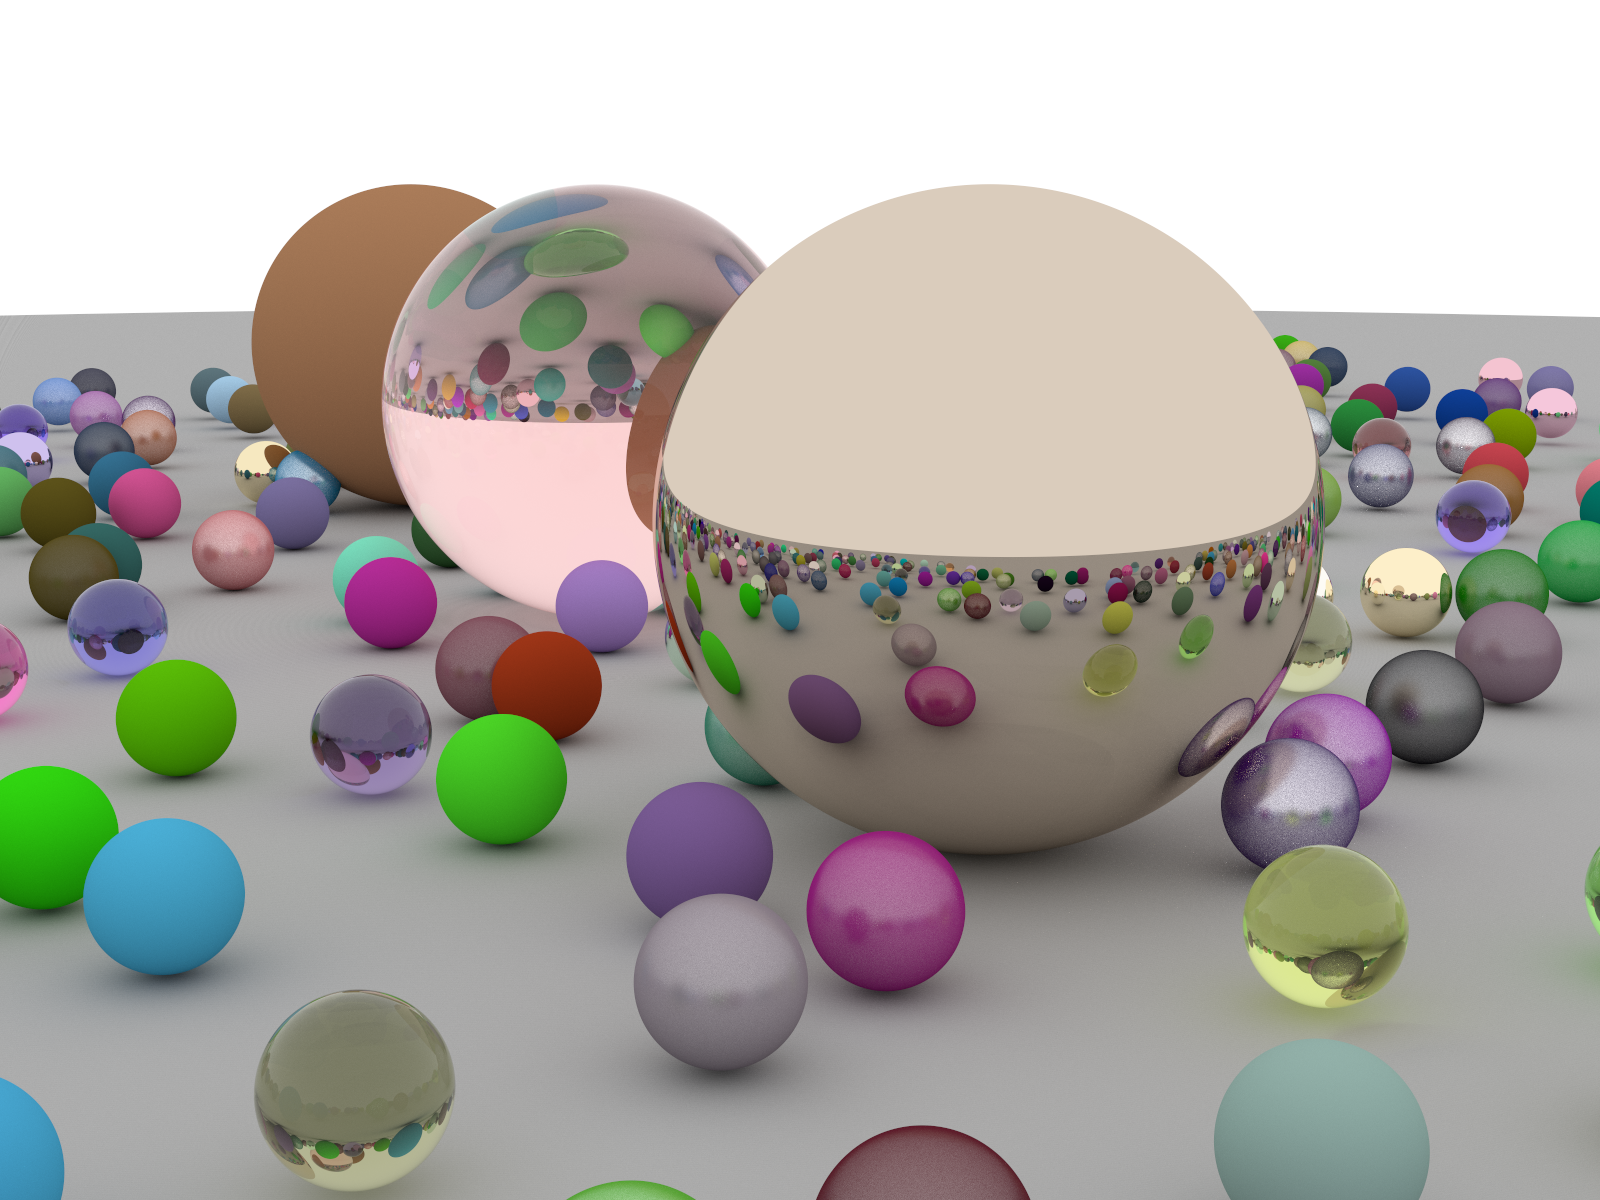
\includegraphics[width=\textwidth]{./fig/pathtracer-result-04-2.png}}
\only<4>{\includegraphics[width=\textwidth]{./fig/pathtracer-result-11-1.png}}
\only<5>{\includegraphics[width=\textwidth]{./fig/pathtracer-result-13-1.png}}
\end{minipage}\hfill
\begin{minipage}{.49\textwidth}
\only<1>{\includegraphics[width=\textwidth]{./fig/pathtracer-result-02.png}}
\only<2>{\includegraphics[width=\textwidth]{./fig/pathtracer-result-04.png}}
\only<3>{\includegraphics[width=\textwidth]{./fig/pathtracer-result-05-2.png}}
\only<4>{\includegraphics[width=\textwidth]{./fig/pathtracer-result-12-3.png}}
\only<5>{\includegraphics[width=\textwidth]{./fig/pathtracer-result-15-3.png}}
\end{minipage}\hfill
\end{frame}

\begin{frame}
\frametitle{\insertsection}
In this lecture: Physically based Path Tracing\\~\\
Conceptual prerequisites:
\begin{itemize}
\item Rasterization-based rendering, e.g. OpenGL
\item Ray tracing principle (but there will be a repetition)
\item Pinhole camera model
\item Basic affine transformations
\item Triangle-based geometry
\item Basic texturing
\end{itemize}
Practical prerequisites:
\begin{itemize}
\item Familiarity with C++
\item Basic familiarity with some GLSL-style types and functions,
    e.g.~\code{vec3}, \code{cosTheta = dot(-I, N)}
\item Note: we will only use CPU-based C++, not GPU programming!
\end{itemize}
\end{frame}

\begin{frame}
\frametitle{\insertsection}
In this lecture: Physically based Path Tracing\\~\\
Many topics of this lecture will be relevant to all rendering methods,\\ not just Path Tracing:
\begin{itemize}
\item Physically based material models
\item Texture filtering, mip maps, anisotropy etc
\item Advanced texturing, normal maps, environment maps etc
\item Procedural textures, noise-based textures
\item Random number sequences for sampling
\item Advanced lens and camera models
\item High Dynamic Range and Tone Mapping
\end{itemize}
\end{frame}

\begin{frame}
\frametitle{\insertsection}
Recommended literature:\\[-1ex]
\begin{minipage}[t]{.48\textwidth}
\centerline{\includegraphics[width=.73\textwidth]{./fig/rtiow.png}}
\footnotesize
\begin{itemize}
\item \url{https://raytracing.github.io/}
\item Implementation only, no theory!
\item First and second book highly recommended; instead of third book I recommend the
corresponding chapters of $\rightarrow$
\end{itemize}
\end{minipage}\hfill
\begin{minipage}[t]{.48\textwidth}
\centerline{\includegraphics[width=.6\textwidth]{./fig/pbr.png}}
\footnotesize
\begin{itemize}
\item \url{https://www.pbr-book.org/}
\item All the topics, thorough coverage, with implementation
\item Comes with the \code{pbrt} renderer
\item A previous edition won an Oscar
\item The definitive resource on the topic!
\end{itemize}
\end{minipage}
\end{frame}

\section{Ray and Path Tracing Basic Ideas}

\begin{frame}
\frametitle{\insertsection}
Models of light and light transport\\~\\~\\
\begin{minipage}{0.29\textwidth}
\centerline{\includegraphics[width=\textwidth]{./fig/optics-models.pdf}}
\end{minipage}\hfill
\begin{minipage}{0.7\textwidth}
\begin{itemize}
\item Quantum Optics: quantum phenomena, fluorescence and phosphorescence
\item Maxwell's Equations: polarization, electro-magnetic field
\item Scalar Wave Optics: interference, diffraction theory %, resolution limit
\item Geometric Optics: emission, refraction and reflection
\end{itemize}
\end{minipage}\\~\\~\\~\\
In this lecture, we only use Geometric Optics:\\
Light transport is based on light rays
\end{frame}

\begin{frame}[label=intro-light-types]
\frametitle{\insertsection}
Different types of light sources typically used in Rasterization\\~\\
\begin{minipage}{.33\textwidth}
\includegraphics[width=\textwidth]{./fig/lightsource-directional.pdf}
\end{minipage}\hfill
\begin{minipage}{.33\textwidth}
\includegraphics[width=\textwidth]{./fig/lightsource-point.pdf}
\end{minipage}\hfill
\begin{minipage}{.33\textwidth}
\includegraphics[width=\textwidth]{./fig/lightsource-spot.pdf}
\end{minipage}\\~\\
\begin{minipage}[t]{.33\textwidth}
Directional Light
\begin{itemize}
\item Infinite distance
\item Parallel rays
\end{itemize}
\end{minipage}\hfill
\begin{minipage}[t]{.33\textwidth}
Point Light
\begin{itemize}
\item One point
\item Isotropic rays
\end{itemize}
\end{minipage}\hfill
\begin{minipage}[t]{.33\textwidth}
Spot Light
\begin{itemize}
\item One point
\item Beam direction
\item Beam angle
\end{itemize}
\end{minipage}\\
\end{frame}

\begin{frame}[label=intro-area-light]
\frametitle{\insertsection}
In physically based rendering: Area Lights
\begin{itemize}
\item Areas or objects that emit light
\item In rasterization: approximated with multiple
point lights
\end{itemize}~\\
\begin{minipage}{.48\textwidth}
    \includegraphics[width=\textwidth]{./fig/lightsource-area-simple.pdf}\hfill
\end{minipage}\hfill
\begin{minipage}{.48\textwidth}
    \includegraphics[width=\textwidth]{./fig/lightsource-area-complex.pdf}
\end{minipage}
\end{frame}

\begin{frame}
\frametitle{\insertsection}
Why do we see objects?
\begin{itemize}
\item<1-> Light sources send light rays
\item<2-> Light rays are perceived by our eye or recorded by a sensor
\item<3-> Light rays are reflected by objects in the scene\\
    depending on geometry and material
\end{itemize}
\vfill
\only<1>{\centerline{\includegraphics[width=.6\textwidth]{./fig/light-transport-0.pdf}}}
\only<2>{\centerline{\includegraphics[width=.6\textwidth]{./fig/light-transport-1.pdf}}}
\only<3-4>{\centerline{\includegraphics[width=.6\textwidth]{./fig/light-transport-3.pdf}}}
%\only<4>{\centerline{\includegraphics[width=.6\textwidth]{./fig/light-transport-3.pdf}}}
\vfill
\visible<4>{
    \vspace*{-\baselineskip}
    \begin{itemize}
    \item Assumption: light travels in vacuum\\ and only interacts at object surfaces
    \end{itemize}
    }
\end{frame}

\begin{frame}
\frametitle{\insertsection}
Light interaction at object surfaces
\begin{itemize}
\item Diffuse reflection
    \begin{itemize}
    \item Also sometimes called matte or Lambertian (for perfectly diffuse)
    \item Models \emph{micro-scale} subsurface scattering: light penetrates the object,
    scatters around, then leaves the object
    \item Light is filtered by the material: its color is changed
    \item Visible from all directions
    \end{itemize}
\end{itemize}
\centerline{\includegraphics[width=.5\textwidth]{./fig/reflection-diffuse-physical.pdf}}
\end{frame}

\begin{frame}[label=intro-diffuse]
\frametitle{\insertsection}
Diffuse surfaces reflect light in all directions.
\only<1>{\centerline{\includegraphics[width=.8\textwidth]{./fig/reflection-diffuse-0.pdf}}}
\only<2>{\centerline{\includegraphics[width=.8\textwidth]{./fig/reflection-diffuse-1.pdf}}}
\only<3>{\centerline{\includegraphics[width=.8\textwidth]{./fig/reflection-diffuse-2.pdf}}}
\only<4>{\centerline{\includegraphics[width=.8\textwidth]{./fig/reflection-diffuse-3.pdf}}}
\begin{itemize}
\item<2-> The perceived brightness does not depend on the view point.
\item<3-> A "higher" light source leads to stronger illumination.
\item<4-> The perceived brightness depends on the \emph{incidence angle}.
\end{itemize}
\end{frame}

\begin{frame}
\frametitle{\insertsection}
Light interaction at object surfaces
\begin{itemize}
\item Glossy reflection
    \begin{itemize}
    \item Also sometimes called specular or shiny
    \item Models \emph{micro-scale} reflection at the surface, from smooth to rough
    \item Light scatters at the surface: its color is often unchanged by the
    material
    \item Appearance changes with angle
    \item Extreme case: perfect mirror
    \end{itemize}
\end{itemize}
\centerline{\includegraphics[width=.5\textwidth]{./fig/reflection-glossy-physical.pdf}}
\end{frame}

\begin{frame}[label=intro-mirroring]
\frametitle{\insertsection}
Perfect mirroring surfaces reflect light in one direction.
\only<1>{\centerline{\includegraphics[width=.8\textwidth]{./fig/reflection-perfect-mirror-0.pdf}}}
\only<2>{\centerline{\includegraphics[width=.8\textwidth]{./fig/reflection-perfect-mirror-1.pdf}}}
\only<3>{\centerline{\includegraphics[width=.8\textwidth]{./fig/reflection-perfect-mirror-2.pdf}}}
\only<4>{\centerline{\includegraphics[width=.8\textwidth]{./fig/reflection-perfect-mirror-3.pdf}}}
\vspace*{-1ex}
\begin{itemize}
\item<2-> The point light source is only visible if the ray hits the eye directly.
\item<3-> From a different viewpoint, the light source would not be visible at
this surface point\ldots{}
\item<4-> \ldots{} but maybe at a different surface point.
\end{itemize}
\end{frame}

\begin{frame}[label=intro-glossy]
\frametitle{\insertsection}
Glossy surfaces scatter light.
\only<1>{\centerline{\includegraphics[width=.8\textwidth]{./fig/reflection-glossy-0.pdf}}}
\only<2>{\centerline{\includegraphics[width=.8\textwidth]{./fig/reflection-glossy-1.pdf}}}
\only<3>{\centerline{\includegraphics[width=.8\textwidth]{./fig/reflection-glossy-2.pdf}}}
\only<4>{\centerline{\includegraphics[width=.8\textwidth]{./fig/reflection-glossy-3.pdf}}}
\vspace*{-1ex}
\begin{itemize}
\item<2-> Maximum brightness is often perceived at the reflection angle.
\item<3-> Perceived brightness often depends on the angle between view ray and
reflection ray\ldots{}
\item<4-> \ldots{} and on the roughness of the surface.
\end{itemize}
\end{frame}

\begin{frame}
\frametitle{\insertsection}
Light interaction at object surfaces
\begin{itemize}
\item Diffuse reflection
\item Glossy reflection
\item Often combined into one material model
\item More on that later
\end{itemize}
\centerline{\includegraphics[width=.7\textwidth]{./fig/reflection-diffuse-and-glossy.pdf}}
\end{frame}

\begin{frame}
\frametitle{\insertsection}
How do we create an image by tracing light rays?
\begin{itemize}
\item<1-> Create light rays from the camera center\\ through every image pixel
\item<2-> Find the intersection of the light ray with a scene object
\item<3-> Compute the illumination at this intersection
\end{itemize}
\vfill
\only<1>{\centerline{\includegraphics[width=.6\textwidth]{./fig/ray-tracing-0.pdf}}}
\only<2>{\centerline{\includegraphics[width=.6\textwidth]{./fig/ray-tracing-1.pdf}}}
\only<3-4>{\centerline{\includegraphics[width=.6\textwidth]{./fig/ray-tracing-2.pdf}}}
\only<5>{\centerline{\includegraphics[width=.6\textwidth]{./fig/ray-tracing-3.pdf}}}
\vfill
\visible<4-5>{
    \vspace*{-\baselineskip}
    \begin{itemize}
    \item Only direct illumination! \only<5>{What about \emph{global} illumination?}
    \end{itemize}
    }
\end{frame}

\begin{frame}
\frametitle{\insertsection}
Direct vs Global Illumination\\~\\
\begin{minipage}{.48\textwidth}
\includegraphics[width=\textwidth]{./fig/cornellbox-direct.png}
\end{minipage}\hfill
\begin{minipage}{.48\textwidth}
\includegraphics[width=\textwidth]{./fig/cornellbox-pathtracing.png}
\end{minipage}
\end{frame}

\begin{frame}[label=idea-global-light-paths]
\frametitle{\insertsection}
Global Illumination with Light Paths\only<3->{: Basic Idea}
\begin{itemize}
\item<1-> At each intersection, light is reflected in \emph{many} directions
\item<2-> Extended ray tracing would require exponential ray splits
\item<3-> Instead: trace individual paths that take \emph{random} choices
\end{itemize}
\vfill
\only<1>{\centerline{\includegraphics[width=.6\textwidth]{./fig/path-tracing-0.pdf}}}
\only<2>{\centerline{\includegraphics[width=.6\textwidth]{./fig/path-tracing-0.pdf}}}
\only<3>{\centerline{\includegraphics[width=.6\textwidth]{./fig/path-tracing-paths-0.pdf}}}
\only<4>{\centerline{\includegraphics[width=.6\textwidth]{./fig/path-tracing-paths-1.pdf}}}
\only<5>{\centerline{\includegraphics[width=.6\textwidth]{./fig/path-tracing-paths-2.pdf}}}
\only<6>{\centerline{\includegraphics[width=.6\textwidth]{./fig/path-tracing-paths-3.pdf}}}
\only<7>{\centerline{\includegraphics[width=.6\textwidth]{./fig/path-tracing-paths-4.pdf}}}
\only<8>{\centerline{\includegraphics[width=.6\textwidth]{./fig/path-tracing-paths-5.pdf}}}
\vfill
\visible<5->{
    \vspace*{-\baselineskip}
    \begin{itemize}
    \item Averaging many such paths approximates global illumination
    \end{itemize}
    }
\end{frame}

\begin{frame}[label=idea-summary]
\frametitle{\insertsection}
Summary of basic ideas:
\begin{itemize}
\item Area light sources emit light
\item Light rays interact at object surfaces
\item Scattered/reflected light rays travel further through the scene
\item Path tracing starts at the camera center and creates
random paths through the scene towards a light source
\item For each pixel, many paths are traced and their contributions averaged
\end{itemize}
~\\
Now we need a proper physically based model for all of this:\\
~\\
\centerline{\textbf{The Rendering Equation}}
\end{frame}

\lecture{}{part2}
\ifthenelse{\boolean{partmode}}{
    \begin{noframenumber}
    \section{Repetition}
    \againframe{idea-global-light-paths}
    \againframe{idea-summary}
    \end{noframenumber}
}{}

\section{Radiometry}

\begin{frame}
\frametitle{\insertsection}
Solid Angle\\
Which angle does an object cover when viewed from a surface point?\\
~\\
\begin{minipage}{.48\textwidth}
2D\\[-\baselineskip]
\centerline{\includegraphics[height=.35\textheight]{./fig/solid-angle-2d.pdf}}
\vspace{-\baselineskip}
\begin{itemize}
\item Project the object onto the unit circle
\item Measure the arc length of the projection
\item $\omega \in [0,\pi]$\\
(whole circle arc length $2\pi$)
\end{itemize}
\end{minipage}\hfill
\begin{minipage}{.48\textwidth}
3D\\[-\baselineskip]
\centerline{\includegraphics[height=.35\textheight]{./fig/solid-angle-3d.pdf}}
\vspace{-\baselineskip}
\begin{itemize}
\item Project the object onto the unit sphere
\item Measure the area of the projection
\item $\omega \in [0,2\pi]$ steradian [sr]\\
(whole sphere area $4\pi$)
\end{itemize}
\end{minipage}
\end{frame}

\begin{frame}
\begin{textblock}{0.45}(0.5,0.36)\includegraphics[width=\textwidth]{./fig/radiance.pdf}\end{textblock}
\frametitle{\insertsection}
Radiometric Quantities
\begin{itemize}
\item Radiant energy $Q$ [J]:
Amount of energy
\item Radiant flux $\Phi =\frac{\partial Q}{\partial t}$ [W=J/s]:
Radiant energy per time
%\item \textcolor{gray}{Radiant intensity $I = \frac{\partial \Phi}{\partial
%\omega}$ [W/sr]: Radiant flux $\Phi$ from a solid angle $\omega$}
%\item \textcolor{gray}{Radiant flux density $u = \frac{\partial \Phi}{\partial
%A}$ [W/$m^2$]: Radiant flux $\Phi$ that "passes" a surface area $A$}
\item[~] ~
\item \textbf{Radiance} $L = \frac{\partial^2\Phi}{\cos\theta~\partial A~\partial \omega}$ [W/$m^2$/sr]:\\
Radiant flux $\Phi$
that "passes"\\ an area $A$
from a solid angle $\omega$\\
in a direction given by $\theta$
\item[~] ~
\item Light transport along a light path\\ is expressed in radiance
\item Sensor response is\\ proportional to radiance
\end{itemize}
\end{frame}

\begin{frame}[label=radiometry-light-at-surface]
\begin{textblock}{0.43}(0.55,0.01)\includegraphics[width=\textwidth]{./fig/brdf.pdf}\end{textblock}
\begin{textblock}{0.40}(0.57,0.58)\includegraphics[width=\textwidth]{./fig/attenuation-cos-theta.pdf}\end{textblock}
\frametitle{\insertsection}
Light interacting with a surface\\
\begin{itemize}
\item Surface point $x$ with normal vector $\vec{n}$
\item Directions relative to $x, \vec{n}$:
    \begin{itemize}
    \item Polar angle $\theta$
    \item Azimuth angle $\varphi$
    \end{itemize}
\item Incoming light direction $\omega_i=(\theta_i,\varphi_i)$
\item Outgoing light direction $\omega_o=(\theta_o,\varphi_o)$
\item[~] ~
\item The incoming radiance $L_i$ from $\omega_i$ is reflected to $\omega_o$:\\
    $L_o(x, \omega_o) = L_i(x,\omega_i)~f(x,\omega_i,\omega_o)\cos\theta_i$
\item Function $f$: \emph{Bidirectional Reflectance\\ Distribution Function
(BRDF)}\\Describes the material properties
\item Attenuation term $\cos\theta_i$\\
corresponds to projection of solid angle onto plane
\end{itemize}
\end{frame}

\begin{frame}[label=radiometry-brdf]
\begin{textblock}{0.5}(0.49,0.19)\includegraphics[width=\textwidth]{./fig/helmholtz-reciprocity.pdf}\end{textblock}
\frametitle{\insertsection}
BRDF: Bidirectional Reflectance Distribution Function\\
~\\Properties of physically plausible BRDFs:
\begin{itemize}
\item Positivity: $f \geq 0$\\
No negative radiance.
\item Helmholtz reciprocity:\\
    $f(x,\omega_i,\omega_o) = f(x,\omega_o,\omega_i)$
\item Energy conservation:
    $\int\limits_\Omega
    f(x,\omega_i,\omega_o)~\cos{\theta_o} d\omega_o \le
    1\quad\forall\omega_i$\\
    Absorption is possible, self-emission is not possible.
\end{itemize}
Simplest example: perfect diffuse reflection (Lambertian reflector)
\begin{itemize}
\item $f = \frac{a}{\pi}$ with albedo $a \in [0,1]$
\item Why divide by $\pi$? To ensure energy conservation!\\
$\int\limits_\Omega \frac{a}{\pi}~\cos{\theta_o} d\omega_o = \frac{a}{\pi}
\int\limits_\Omega \cos{\theta_o} d\omega_o = \frac{a}{\pi} \cdot \pi = a$
\item Compare $L_o(x, \omega_o) =
L_i(x,\omega_i)~\frac{a}{\pi}\cos\theta_i$ with Phong's $I_d \cdot k_d \cdot \vec{n}\vec{l}$
\end{itemize}
\end{frame}

\begin{frame}
\begin{textblock}{0.6}(0.2,0.3)
\only<1>{~}
\only<2>{\includegraphics[width=\textwidth]{./fig/rendering-equation-2.pdf}}
\only<3>{\includegraphics[width=\textwidth]{./fig/rendering-equation-3.pdf}}
\only<4>{\includegraphics[width=\textwidth]{./fig/rendering-equation-4.pdf}}
\only<5>{\includegraphics[width=\textwidth]{./fig/rendering-equation-5.pdf}}
\only<6>{\includegraphics[width=\textwidth]{./fig/rendering-equation-6.pdf}}
\only<7>{\includegraphics[width=\textwidth]{./fig/rendering-equation-7.pdf}}
\only<8>{\includegraphics[width=\textwidth]{./fig/rendering-equation-8.pdf}}
\end{textblock}
\begin{textblock}{1.0}(0.0,0.8)
\begin{itemize}
\item[~] ~
\only<2>{\item Radiance from $x$ to camera center through image pixel}
\only<3>{\item Emitted radiance (here zero, because this is not a light source)}
\only<4>{\item Integral over all incoming directions $\omega_i$ of the hemisphere}
\only<5>{\item Incoming radiance from directions $\omega_i$}
\only<6>{\item BRDF (material property) and attenuation term}
\only<7>{\item Recursively for all light paths}
\only<8>{\item For a light source, $L_e > 0$}
\end{itemize}
\end{textblock}
\frametitle{\insertsection}
{\setlength{\fboxsep}{0pt}
The rendering equation\\
    ~\\
\only<1>{$\displaystyle L_o(x, \omega_o) = L_e(x, \omega_o) + \int\limits_\Omega
    L_i(x,\omega_i)~f(x,\omega_i,\omega_o)~\cos\theta_i~d\omega_i$\\}
\only<2>{$\displaystyle \colorbox{green!30}{$L_o(x, \omega_o)$} = L_e(x, \omega_o) + \int\limits_\Omega
    L_i(x,\omega_i)~f(x,\omega_i,\omega_o)~\cos\theta_i~d\omega_i$\\}
\only<3>{$\displaystyle L_o(x, \omega_o) = \colorbox{green!30}{$L_e(x, \omega_o)$} + \int\limits_\Omega
    L_i(x,\omega_i)~f(x,\omega_i,\omega_o)~\cos\theta_i~d\omega_i$\\}
\only<4>{$\displaystyle L_o(x, \omega_o) = L_e(x, \omega_o) + \colorbox{green!30}{$\ds \int\limits_\Omega$}\,
    L_i(x,\omega_i)~f(x,\omega_i,\omega_o)~\cos\theta_i~\colorbox{green!30}{$d\omega_i$}$\\}
\only<5>{$\displaystyle L_o(x, \omega_o) = L_e(x, \omega_o) + \int\limits_\Omega
    \colorbox{green!30}{$L_i(x,\omega_i)$}~f(x,\omega_i,\omega_o)~\cos\theta_i~d\omega_i$\\}
\only<6>{$\displaystyle L_o(x, \omega_o) = L_e(x, \omega_o) + \int\limits_\Omega
    L_i(x,\omega_i)~\colorbox{green!30}{$f(x,\omega_i,\omega_o)~\cos\theta_i$}~d\omega_i$\\}
\only<7>{$\displaystyle L_o(x, \omega_o) = L_e(x, \omega_o) + \int\limits_\Omega
    L_i(x,\omega_i)~f(x,\omega_i,\omega_o)~\cos\theta_i~d\omega_i$\\}
\only<8>{$\displaystyle L_o(x, \omega_o) = \colorbox{green!30}{$L_e(x, \omega_o)$} + \int\limits_\Omega
    L_i(x,\omega_i)~f(x,\omega_i,\omega_o)~\cos\theta_i~d\omega_i$\\}
}
\end{frame}

\begin{frame}
\frametitle{\insertsection}
\ldots{} or this \ldots{}\\~\\[-1ex]
\includegraphics[width=\textwidth]{./fig/rendering-equation-explainer.png}\\
{\tiny Source:
\href{https://twitter.com/levork/status/609603797258600448}{Tweet} by Julian
Fong (@levork) 2015-06-13}
\end{frame}


\section{Path Tracing}

\begin{frame}
\frametitle{\insertsection}
The rendering equation\\
    ~\\
$\displaystyle L_o(x, \omega_o) = L_e(x, \omega_o) + \int\limits_\Omega
    L_i(x,\omega_i)~f(x,\omega_i,\omega_o)~\cos\theta_i~d\omega_i$\\
~\\[-1ex]
Numerical approximation of an integral: $\ds \int\limits_a^b f(x)dx \approx \frac{b-a}{N} \sum\limits_{i=1}^N f(x_i)$\\
\begin{minipage}{.48\textwidth}
\centerline{Deterministic sampling}
\centerline{(Riemann sum)}
\only<1>{\centerline{\includegraphics[width=.9\textwidth]{./fig/integration-riemann-4.pdf}}}
\only<2>{\centerline{\includegraphics[width=.9\textwidth]{./fig/integration-riemann-8.pdf}}}
\only<3>{\centerline{\includegraphics[width=.9\textwidth]{./fig/integration-riemann-12.pdf}}}
\end{minipage}\hfill
\begin{minipage}{.48\textwidth}
\centerline{Stochastic sampling}
\centerline{with uniform distribution}
\only<1>{\centerline{\includegraphics[width=.9\textwidth]{./fig/integration-stochastic-4.pdf}}}
\only<2>{\centerline{\includegraphics[width=.9\textwidth]{./fig/integration-stochastic-8.pdf}}}
\only<3>{\centerline{\includegraphics[width=.9\textwidth]{./fig/integration-stochastic-12.pdf}}}
\end{minipage}
\end{frame}

\begin{frame}
\frametitle{\insertsection}
Why stochastic sampling?
\begin{itemize}
\item[\textcolor{DarkRed}{--}] Slower convergence than deterministic sampling
\item[\textcolor{DarkGreen}{+}] New samples can be added without resampling
\item[\textcolor{DarkGreen}{\textbf{+}}] Most importantly: Monte Carlo integration gives access to\\
    crucial optimizations (in a following lecture)
\item[\textcolor{DarkGreen}{+}] Can give \emph{visually} better results.
Example: Antialiasing when sampling high frequency signals on a coarse grid\\
    \only<1>{\includegraphics[width=.75\textwidth]{./fig/sampling-regular-vs-stochastic-0.pdf}}
    \only<2>{\includegraphics[width=.75\textwidth]{./fig/sampling-regular-vs-stochastic-1.pdf}}
    \only<3>{\includegraphics[width=.75\textwidth]{./fig/sampling-regular-vs-stochastic-2.pdf}}
\end{itemize}
\end{frame}

\begin{frame}[label=path-tracing-rendering-equation]
\frametitle{\insertsection}
Path Tracing: Sampling the Rendering Equation\\~\\
$\displaystyle L_o(x, \omega_o) = L_e(x, \omega_o) + \int\limits_\Omega
    L_i(x,\omega_i)~f(x,\omega_i,\omega_o)~\cos\theta_i~d\omega_i$\\
~\\
\vfill
\only<1>{\centerline{\includegraphics[width=.6\textwidth]{./fig/path-tracing-0.pdf}}}
\only<2>{\centerline{\includegraphics[width=.6\textwidth]{./fig/path-tracing-paths-1.pdf}}}
\only<3>{\centerline{\includegraphics[width=.6\textwidth]{./fig/path-tracing-paths-2.pdf}}}
\only<4>{\centerline{\includegraphics[width=.6\textwidth]{./fig/path-tracing-paths-3.pdf}}}
\only<5>{\centerline{\includegraphics[width=.6\textwidth]{./fig/path-tracing-paths-4.pdf}}}
\only<6>{\centerline{\includegraphics[width=.6\textwidth]{./fig/path-tracing-paths-5.pdf}}}
\vfill
\visible<2->{
    \vspace*{-\baselineskip}
    \begin{itemize}
    \item Each light path is a sample
    \end{itemize}
    }
\end{frame}

\section{Brute Force Path Tracing}

\begin{frame}[label=path-tracing-brute-force-stochastic]
\frametitle{\insertsection}
Path Tracing: Sampling the Rendering Equation\\
$\displaystyle L_o(x, \omega_o) = L_e(x, \omega_o) + \int\limits_\Omega
    L_i(x,\omega_i)~f(x,\omega_i,\omega_o)~\cos\theta_i~d\omega_i$\\
~\\
Stochastic integration:\\
$\ds\begin{aligned}
    \int\limits_a^b f(x)dx &\approx \frac{b-a}{N} \sum\limits_{i=1}^N f(x_i)\\
    &=\frac{1}{N}\sum\limits_{i=1}^N \frac{f(x_i)}{p(x_i)}\quad\text{with}\quad
    p(x_i)=\frac{1}{b-a}\end{aligned}$\\
~\\
Applied to the Rendering Equation: integration over the hemisphere $\Omega$\\
$\ds \int\limits_\Omega f(\omega_i)dx \approx
\frac{1}{N}\sum\limits_{i=1}^N
     \frac{f(\omega_i)}{p(\omega_i)}\quad\text{with}\quad
     p(\omega_i)=\frac{1}{2\pi}$\\
\end{frame}

\begin{frame}[fragile]
\frametitle{\insertsection}
Brute Force Path Tracing: Pseudo Code\\~\\
\begin{lstlisting}
for (pixels p in image) {
    image[p] = 0;
    for (sample = 0; sample < sampleCount; sample++) {
        Ray ray;
        ray.origin = camera.center();
        ray.direction = camera.getRay(p, s);
        /***********************************************/
        /* compute radiance for this light path sample */
        /***********************************************/
        image[p] += radiance / sampleCount;
    }
}
\end{lstlisting}
\end{frame}

\begin{frame}[label=path-tracing-brute-force-path]
\frametitle{\insertsection}
Brute Force Path Tracing: Pseudo Code\\~\\
Calculating the radiance $L = L_o(x, \omega_o)$ for one path:
\begin{itemize}
\item Let's say we have $N$ intersections $x_k, k=1,\ldots, N$.\\
    The $N$th intersection is a dominant light source,\\ % (or environment map),
    so we end the path there.
\item With the following shortcut notation
    \begin{itemize}
    \item $L_k = L_e(x_k, (\omega_o)_k)$
    \item $a_k = f(x_k, (\omega_i)_k, (\omega_o)_k) \cos((\theta_i)_k) / p(\omega_i)$
    \end{itemize}
    we have:\\
    $L = L_1 + a_1(L_2 + a_2(L_3 + a_3(L_4 + \ldots + a_{N-1}L_N)\ldots)$
    $\hphantom{L} = 1\cdot L_1 + a_1\cdot L_2 + a_1a_2\cdot L_3 + a_1a_2a_3\cdot L_4 + \ldots + a_1\ldots a_{N-1}\cdot L_N$
    $\hphantom{L} = \sum\limits_{k=1}^N (\prod\limits_{j=1}^{k-1} a_j)L_k$
\item Implementation:
    \begin{itemize}
    \item Variable \code{radiance} as a running sum
    \item Variable \code{throughput} as a running product
    \end{itemize}
\end{itemize}
\end{frame}

\begin{frame}[fragile]
\frametitle{\insertsection}
Brute Force Path Tracing: Implementation\\
\begin{lstlisting}
/* compute radiance for this light path sample: */
radiance = 0;
throughput = 1;
for (segment = 0; segment < maxsegments; segment++) {
    x = intersect(ray, scene);
    if (noIntersection) break;
    n = surfaceNormal(x);
    radiance += throughput * Le(x, -ray.direction);
    if (pathStopsHere(x)) break;
    newDirection = randomUniformOnHemisphere(x, n);
    brdf = f(x, -newDirection, -ray.direction);
    cosTheta = dot(n, newDirection);
    throughput *= brdf * cosTheta;
    throughput /= 1.0f / (2.0f * pi);
    ray.origin = x;
    ray.direction = newDirection;
}
\end{lstlisting}
\end{frame}

\begin{frame}
\frametitle{\insertsection}
Brute Force Path Tracing: Example\\
~\\
~\\
\begin{minipage}[t]{.33\textwidth}
\includegraphics[width=\textwidth]{./fig/cornellbox-bruteforce-4spp.png}
\centerline{4 samples per pixel}
\centerline{(spp)}
\end{minipage}\hfill
\begin{minipage}[t]{.33\textwidth}
\includegraphics[width=\textwidth]{./fig/cornellbox-bruteforce-16spp.png}
\centerline{16 spp}
\end{minipage}\hfill
\begin{minipage}[t]{.33\textwidth}
\includegraphics[width=\textwidth]{./fig/cornellbox-bruteforce-256spp.png}
\centerline{256 spp}
\end{minipage}
\end{frame}

\begin{frame}[label=path-tracing-brute-force-example]
\frametitle{\insertsection}
Brute Force Path Tracing: Example\\
~\\
~\\
\begin{minipage}[t]{.33\textwidth}
\includegraphics[width=\textwidth]{./fig/cornellbox-bruteforce-1024spp.png}
\centerline{1024 spp\hphantom{Fp}}
\end{minipage}\hfill
\begin{minipage}[t]{.33\textwidth}
\includegraphics[width=\textwidth]{./fig/cornellbox-bruteforce-4096spp.png}
\centerline{4096 spp\hphantom{Fp}}
\end{minipage}\hfill
\begin{minipage}[t]{.33\textwidth}
\only<1>{~}
\only<2>{\includegraphics[width=\textwidth]{./fig/cornellbox-full-monte-carlo-64spp.png}
\centerline{Outlook:}
\centerline{with proper Monte}
\centerline{Carlo techniques}
\centerline{64 spp}}
\end{minipage}
\end{frame}

\begin{frame}
\frametitle{\insertsection}
Brute Force Path Tracing: Antialiasing\\
~\\
\begin{minipage}{.25\textwidth}
\includegraphics[width=\textwidth]{./fig/cornellbox-antialiasing-off.png}
\end{minipage}~~~~
\begin{minipage}{.21\textwidth}
\includegraphics[width=\textwidth]{./fig/cornellbox-antialiasing-off-cutout.png}
\end{minipage}~~~~
\begin{minipage}{.3\textwidth}
\includegraphics[width=\textwidth]{./fig/antialiasing-1.pdf}
\end{minipage}\\
\begin{minipage}{.25\textwidth}
\includegraphics[width=\textwidth]{./fig/cornellbox-antialiasing-on.png}
\end{minipage}~~~~
\begin{minipage}{.21\textwidth}
\includegraphics[width=\textwidth]{./fig/cornellbox-antialiasing-on-cutout.png}
\end{minipage}~~~~
\begin{minipage}{.3\textwidth}
\includegraphics[width=\textwidth]{./fig/antialiasing-2.pdf}
\end{minipage}\\
\end{frame}

\begin{frame}
\frametitle{\insertsection}
Brute Force Path Tracing: Motion Blur\\
~\\
\begin{minipage}[t]{0.49\textwidth}
\begin{itemize}
\item Define an exposure time interval for your image: $[t_0, t_1]$
\item When creating a new path, assign a random time $t\in [t_0,t_1]$
\item Consider this time when computing intersections with the scene
\end{itemize}
\end{minipage}\hfill
\begin{minipage}[t]{0.49\textwidth}
~\\[-\baselineskip]
\includegraphics[width=\textwidth]{./fig/cornellbox-motionblur.png}
\end{minipage}
\end{frame}

\begin{frame}[label=path-tracing-brute-force-implementation]
\frametitle{\insertsection}
Brute Force Path Tracing: First Implementation\\~\\
What do we need?
\begin{enumerate}
\item Ray
\item Camera
\item Surfaces
\item Material
\item Hemisphere sampling
\end{enumerate}
\end{frame}

\begin{frame}
\frametitle{\insertsection}
\begin{enumerate}
\item[\labelname{1}] Ray
    \begin{itemize}
    \item Origin $o$
    \item Direction $d$ with unit length
    \item[~] \includegraphics[width=.5\textwidth]{./fig/ray.pdf}
    \item Point $p$ at distance $\alpha$ along the ray is given as\\
        $p = o + \alpha \cdot d$
    \end{itemize}
\end{enumerate}
\end{frame}

\begin{frame}[fragile]
\frametitle{\insertsection}
\begin{enumerate}
\item[\labelname{1}] Ray
\begin{lstlisting}
class Ray
{
    vec3 origin;
    vec3 direction; // must have unit length!

    Ray(const vec3& o, const vec3& d) :
        origin(o),
        direction(d)
    {
    }

    vec3 at(float a) const
    {
        return origin + a * direction;
    }
};
\end{lstlisting}
\end{enumerate}
\end{frame}

\begin{frame}
\frametitle{\insertsection}
\begin{enumerate}
\item[\labelname{2}] Camera
\begin{itemize}
\item We start with a pinhole camera
\item Frustum definition via top, bottom, left and right parameters\\
    (for simplicity: measured at distance 1)
\item For now, the camera center is fixed at $(0,0,0)$ and looks
along $(0,0,-1)$, with an up vector of $(0,1,0)$
\item This is the canonical camera space known from e.g. OpenGL
\item[~]
    \begin{minipage}{.3\textwidth}
    \includegraphics[width=\textwidth]{./fig/camera.pdf}
    \end{minipage}\hfill
    \begin{minipage}{.5\textwidth}
    Generate ray for normalized image coordinates $p,q \in [0,1]$:\\
    $o = (0,0,0)$\\
    $\vec{d}' = (l + p\cdot (r-l), b + q \cdot(t-b), -1)$\\
    $\vec{d}  = \frac{\vec{d}'}{||\vec{d}'||}$
    \end{minipage}
\end{itemize}
\end{enumerate}
\end{frame}

\begin{frame}[fragile]
\frametitle{\insertsection}
\begin{enumerate}
\item[\labelname{2}] Camera
\begin{lstlisting}
class Camera
{
    float t, b, r, l;

    Camera(float vfov, float aspectRatio) :
        t(std::tan(vfov * 0.5f)),
        b(-t),
        r(t * aspectRatio),
        l(-r)
    {
    }
};
\end{lstlisting}
\end{enumerate}
\end{frame}

\begin{frame}[fragile]
\frametitle{\insertsection}
\begin{enumerate}
\item[\labelname{2}] Camera
\begin{lstlisting}
class Camera
{
    Ray getRay(float p, float q)
    {
        // get origin O and direction D in camera space
        vec3 P = vec3(mix(l, r, p), mix(b, t, q), -1.0f);
        vec3 O = vec3(0.0f);
        vec3 D = P - O;
        // transform (not yet)
        //   O = transormation * O;
        //   D = rotation * D;
        return Ray(O, normalize(D));
    }
};
\end{lstlisting}
\end{enumerate}
\end{frame}

\begin{frame}[fragile]
\frametitle{\insertsection}
\begin{enumerate}
\item[\labelname{3}] Surface
\begin{itemize}
\item Represents the objects in the scene
\item Must be able to tell whether a ray intersects
    \begin{itemize}
    \item Where is the intersection position $p$?
    \item What is the surface normal $\vec{n}$ at $p$?
    \item Which material is at $p$?
    \end{itemize}
\end{itemize}
\begin{lstlisting}
class Surface
{   virtual HitRecord hit(
        const Ray& ray, float amin, float amax)
    { return HitRecord(); }
};
class HitRecord {
    bool haveHit;
    float a;
    vec3 position;
    vec3 normal;
    const Material* material;
};
\end{lstlisting}
\end{enumerate}
\end{frame}

\begin{frame}
\frametitle{\insertsection}
\begin{enumerate}
\item[\labelname{3}] Surface\\
We start with a sphere with center $c$ and radius $r$:\\
\begin{minipage}{.24\textwidth}
\includegraphics[width=\textwidth]{./fig/sphere.pdf}
\end{minipage}\hfill
\begin{minipage}{.64\textwidth}
\begin{itemize}
\item For point p on sphere: $(p-c)\cdot(p-c) = r^2$
\item For point p along ray: $p = o + \alpha \cdot \vec{d}$
\item Intersection: solve for $\alpha$
\end{itemize}
\end{minipage}\\~\\[.5ex]
    $(o + \alpha d - c)\cdot(o + \alpha d -c) = r^2$\\
    $\Leftrightarrow (d\alpha + o-c)(d\alpha + o-c) -r^2 = 0$\\
    $\Leftrightarrow d\cdot d \alpha^2 + 2d\cdot(o-c)\alpha + (o-c)\cdot(o-c)-r^2 = 0$\\
    $\Leftrightarrow \alpha^2 + 2d\cdot(o-c)\alpha + (o-c)\cdot(o-c)-r^2 = 0$\\
    $\Rightarrow \alpha_{1,2} = -d\cdot(o-c) \pm \sqrt{(d\cdot(o-c))^2 - ((o-c)\cdot(o-c)-r^2)}$\\
    ~\\
0, 1, or 2 intersections (use the nearest)
\end{enumerate}
\end{frame}

\begin{frame}[fragile]
\frametitle{\insertsection}
\begin{enumerate}
\item[\labelname{3}] Surface
\begin{lstlisting}
class SurfaceSphere : public Surface {
    virtual HitRecord hit(ray, amin, amax) override {
        vec3 oc = ray.origin - center;
        float e = dot(oc, ray.direction);
        float f = dot(oc, oc) - radius * radius;
        float discriminant = e * e - f;
        HitRecord hr;
        if (discriminant > 0.0f) {
            float a = -e - std::sqrt(discriminant);
            if (a > amin && a < amax)
                hr = constructHitRecord(ray, a);
            else
                a = -e + std::sqrt(discriminant);
                if (a > amin && a < amax) {
                    hr = constructHitRecord(ray, a);
        return hr;
    }
};
\end{lstlisting}
\end{enumerate}
\end{frame}

\begin{frame}[fragile]
\frametitle{\insertsection}
\begin{enumerate}
\item[\labelname{3}] Surface
\begin{lstlisting}
class SurfaceSphere : public Surface
{
    HitRecord constructHitRecord(const Ray& ray, float a)
    {
        vec3 p = ray.at(a);
        vec3 n = normalize(p - center);
        if (dot(n, -ray.direction) < 0.0f) {
            n = -n;
        }
        return HitRecord(a, p, n, material);
    }
};
\end{lstlisting}
\end{enumerate}
\end{frame}

\begin{frame}[fragile]
\frametitle{\insertsection}
\begin{enumerate}
\item[\labelname{4}] Material
\begin{itemize}
\item Describes the interaction with light at the ray/surface interaction
\item Implements the BRDF $f(x,\omega_i,\omega_o)$
\item Implements the emitted radiance function $L_e(x,\omega_o)$
\item In the case of a light source, tells the path tracer to stop a path
\end{itemize}
\begin{lstlisting}
class Material
{
    virtual vec3 Le(const HitRecord& hr, vec3 out) const
    { return vec3(0.0f); }

    virtual bool pathStopsHere() const
    { return false; }

    virtual vec3 brdf(const HitRecord& hr,
        const vec3& in, const vec3& out) const
    { return vec3(0.0f); }
};
\end{lstlisting}
\end{enumerate}
\end{frame}

\begin{frame}[fragile]
\frametitle{\insertsection}
\begin{enumerate}
\item[\labelname{4}] Material
\begin{itemize}
\item We start with a perfectly diffuse (Lambertian) material:\\
$f\equiv \frac{a}{\pi}$ with albedo $a\in[0,1]$
\begin{lstlisting}
class MaterialLambertian : public Material {
    virtual vec3 brdf(hr, in, out) const override
    { return albedo / pi; }
};
\end{lstlisting}
\item and a diffuse light source material:\\
    $L_e \equiv R$ with radiance $R\in[0,\infty)$
\begin{lstlisting}
class MaterialLight : public Material {
    virtual vec3 Le(hr, out) const override
    { return radiance; }
    virtual bool pathStopsHere() const override
    { return true; }
};
\end{lstlisting}
\end{itemize}
\end{enumerate}
\end{frame}

\begin{frame}[fragile]
\frametitle{\insertsection}
\begin{enumerate}
\item[\labelname{5}] Hemisphere Sampling
\begin{itemize}
\item Component 1: A pseudo-random number generator\\
for uniformly distributed numbers in $[0,1)$
\begin{lstlisting}
class Prng
{
    std::mt19937_64 generator;
    std::uniform_real_distribution<float> distrib;

    Prng(unsigned long seed) :
        generator(seed), distrib(0.0f, 1.0f)
    {}

    float in01() { return distrib(generator); }
};
\end{lstlisting}
\end{itemize}
\end{enumerate}
\end{frame}

\begin{frame}
\frametitle{\insertsection}
\begin{enumerate}
\item[\labelname{5}] Hemisphere Sampling
\begin{itemize}
\item Component 2: A function to generate random normalized directions\\~\\
For now: simple rejection sampling and normalization\\~\\
\includegraphics[width=.7\textwidth]{./fig/sampling-uniform-directions.pdf}
\end{itemize}
\end{enumerate}
\end{frame}

\begin{frame}[fragile]
\frametitle{\insertsection}
\begin{enumerate}
\item[\labelname{5}] Hemisphere Sampling
\begin{itemize}
\item Component 2: A function to generate random normalized directions\\~\\
For now: simple rejection sampling and normalization\\
\begin{lstlisting}
class Prng
{
    vec3 inUnitSphere() {
        vec3 p;
        do { p = vec3(2.0f * in01() - 1.0f,
                      2.0f * in01() - 1.0f,
                      2.0f * in01() - 1.0f);
        } while (dot(p, p) >= 1.0f);
        return p;
    }
    vec3 onUnitSphere() {
        return normalize(inUnitSphere());
    }
};
\end{lstlisting}
\end{itemize}
\end{enumerate}
\end{frame}

\begin{frame}[fragile]
\frametitle{\insertsection}
\begin{enumerate}
\item[\labelname{5}] Hemisphere Sampling
\begin{itemize}
\item Component 3: A function to generate a uniformly distributed
direction on the hemisphere around the normal vector $\vec{n}$\\~\\
\begin{minipage}{.35\textwidth}
\includegraphics[width=\textwidth]{./fig/sampling-uniform-hemisphere.pdf}
\end{minipage}\hfill
\begin{minipage}{.5\textwidth}
\begin{lstlisting}
vec3 onUnitHemisphere(
    const vec3& n,
    const vec3& rd)
{
    vec3 d;
    if (dot(rd, n) > 0.0f)
        d = rd;
    else
        d = -rd;
    return d;
}
\end{lstlisting}
\end{minipage}
\end{itemize}
\end{enumerate}
\end{frame}

\begin{frame}[fragile]
\frametitle{\insertsection}
Putting \labelname{1}~--\labelname{5} together, part 1: Create a scene\\
\begin{lstlisting}
MaterialLambertian leftMaterial(vec3(1.0f, 0.2f, 0.2f));
SurfaceSphere leftSphere(vec3(-1.1f, 0.55f, -5.0f), 1.0f,
                    &leftMaterial);
MaterialLambertian rightMaterial(vec3(0.2f, 1.0f, 0.2f));
SurfaceSphere rightSphere(vec3(+1.1f, 0.55f, -5.0f), 1.0f,
                    &rightMaterial);
MaterialLambertian groundMaterial(vec3(0.5f, 0.5f, 0.5f));
SurfaceSphere groundSphere(vec3(0.0f, -100.0f, -5.0f), 99.5f,
                    &groundMaterial);
MaterialLight lightMaterial(vec3(1.0f, 1.0f, 1.0f));
SurfaceSphere lightSphere(vec3(0.0f, 0.0f, -5.0f), 50.0f,
                    &lightMaterial);
std::vector<Surface*> scene;
scene.push_back(&leftSphere);
scene.push_back(&rightSphere);
scene.push_back(&groundSphere);
scene.push_back(&lightSphere);
\end{lstlisting}
\end{frame}

\begin{frame}[fragile]
\frametitle{\insertsection}
Putting \labelname{1}~--\labelname{5} together, part 2: Find the nearest hit in a scene\\
\begin{lstlisting}
HitRecord hit(const std::vector<Surface*>& scene,
              const Ray& ray)
{
    float amin = 0.0001f;
    float amax = FLT_MAX;
    float nearestA = amax;
    HitRecord hr;
    for (size_t i = 0; i < scene.size(); i++) {
        HitRecord tmpHr = scene[i]->hit(ray, amin, amax);
        if (tmpHr.haveHit && tmpHr.a < nearestA) {
            hr = tmpHr;
            amax = hr.a;
        }
    }
    return hr;
}
\end{lstlisting}
\end{frame}

\begin{frame}[fragile]
\frametitle{\insertsection}
Putting \labelname{1}~--\labelname{5} together, part 3: Compute radiance for one path\\
\begin{lstlisting}
vec3 pathSample(scene, ray, prng) {
    vec3 radiance(0.0f), throughput(1.0f);
    for (int segment = 0; segment < maxSegments; segment++) {
        HitRecord hr = hit(scene, ray);
        if (!hr.haveHit) break;
        vec3 out = -ray.direction;
        radiance += throughput * hr.material->Le(hr, out);
        if (hr.material->pathStopsHere()) break;
        vec3 newDir = onHemisph(hr.normal, prng.onSph());
        vec3 in = -newDir;
        vec3 brdf = hr.material->brdf(hr, in, out);
        float cosTheta = dot(hr.normal, newDir);
        throughput *= brdf * cosTheta;
        throughput *= 2.0f * pi;
        ray = Ray(hr.position, newDir);
    }
    return radiance;
}
\end{lstlisting}
\end{frame}

\begin{frame}[fragile]
\frametitle{\insertsection}
Putting \labelname{1}~--\labelname{5} together, part 4: The main loop\\
\begin{lstlisting}
std::vector<vec3> img(width * height);
Camera camera(degrees(60.0f), float(width) / height);
#pragma omp parallel for
for (size_t pixel = 0; pixel < img.size(); pixel++) {
    Prng prng(pixel + 42);
    int y = pixel / width;
    int x = pixel \% width;
    img[y * width + x] = vec3(0.0f);
    for (int i = 0; i < samplesPerPixel; i++) {
        float p = (x + 0.5f) / width;
        float q = (y + 0.5f) / height;
        Ray ray = camera.getRay(p, q);
        img[y * width + x] += radForPath(scene, ray, prng);
    }
    img[y * width + x] /= samplesPerPixel;
}
\end{lstlisting}
\end{frame}

\begin{frame}[label=path-tracing-brute-force-tadaaa]
\frametitle{\insertsection}
Putting \labelname{1}~--\labelname{5} together: Tadaaa!\\~\\
\centerline{\includegraphics[width=.7\textwidth]{./fig/pathtracer-result-01.png}}
\end{frame}

\begin{frame}
\frametitle{\insertsection}
Summary\\~\\
\begin{minipage}[t]{.59\textwidth}
\begin{itemize}
\item The rendering equation describes light transport using physical quantities\\
    $\displaystyle L_o(x, \omega_o) = L_e(x, \omega_o) +
    \int\limits_\Omega
    L_i(x,\omega_i)~f(x,\omega_i,\omega_o)~\cos\theta_i~d\omega_i$\\
\end{itemize}
\end{minipage}\hfill
\begin{minipage}[t]{.39\textwidth}
    \hphantom{~}
    \includegraphics[width=\textwidth]{./fig/path-tracing-0.pdf}
\end{minipage}\\
\begin{minipage}[t]{.59\textwidth}
\begin{itemize}
\item Path tracing approximates the integral using light path samples
\end{itemize}
\end{minipage}\hfill
\begin{minipage}[t]{.39\textwidth}
    \hphantom{~}
    \includegraphics[width=\textwidth]{./fig/path-tracing-paths-5.pdf}
\end{minipage}\\
\vspace*{-\baselineskip}
\begin{itemize}
\item An initial brute force implementation uses random ray reflection directions
    that are uniformly distributed on the hemisphere
\end{itemize}
\end{frame}

\lecture{}{part3}
\ifthenelse{\boolean{partmode}}{
    \begin{noframenumber}
    \section{Repetition}
    \againframe{radiometry-light-at-surface}
    \againframe{radiometry-brdf}
    \againframe{path-tracing-rendering-equation}
    \againframe{path-tracing-brute-force-stochastic}
    \againframe{path-tracing-brute-force-path}
    \againframe{path-tracing-brute-force-example}
    \againframe{path-tracing-brute-force-implementation}
    \againframe{path-tracing-brute-force-tadaaa}
    \end{noframenumber}
}{}

\section{Extending the Brute Force Path Tracer}

\begin{frame}
\frametitle{\insertsection}
Transformations
\begin{itemize}
\item Affine transformations allow animation of camera and/or objects
\item You know affine transformations represented in $4\times 4$ matrices,\\
    especially translation, rotation, scaling
\item Here we use a different representation with separated components:
    \begin{itemize}
    \item Translation: represented as a vector with 3 components
    \item Rotation: represented as a Quaternion
    \item Scaling: represented as a vector with 3 components
    \end{itemize}
\item This allows interpolation of transformations, e.g.~for keyframe
animations
    \begin{itemize}
    \item Linear interpolation of the translation and scaling
    \item Spherical linear interpolation (SLERP) of the rotation
    \end{itemize}
\item And it removes the necessity for normal matrices
    \begin{itemize}
    \item Simply only apply the rotation to direction vectors, omit the
    translation 
    \end{itemize}
\end{itemize}
\end{frame}

\begin{frame}
\frametitle{\insertsection}
Transformations: Reminder / Overview of Quaternions
\begin{itemize}
\item 4 components: $q=(q_x, q_y, q_z, q_w)$
\item Quaternion multiplication $t = r \cdot s$ is defined as\\
    $t_x = r_w s_x + r_x s_w + r_y s_z - r_z s_y$\\
    $t_y = r_w s_y + r_y s_w + r_z s_x - r_x s_z$\\
    $t_z = r_w s_z + r_z s_w + r_x s_y - r_y s_x$\\
    $t_w = r_w s_w - r_x s_x - r_y s_y - r_z s_z$\\
    Associative $(rs)t=r(st)$, not commutative $rs \neq sr$
\item The \emph{conjugate} of a quaternion is $\bar{q} = (-q_x, -q_y, -q_z, q_w)$
\item The \emph{magnitude} of a quaternion is\\
    $|q|=\sqrt{q\bar{q}} = \sqrt{q_x^2 + q_y^2 + q_z^2 + q_w^2}$
\item A \emph{unit quaternion} has magnitude 1
\item The \emph{inverse} of a quaternion is $q^{-1}=\frac{\bar{q}}{|q|^2}$
\end{itemize}
\end{frame}

\begin{frame}
\frametitle{\insertsection}
Transformations: Reminder / Overview of Quaternions
\begin{itemize}
\item In Computer Graphics, unit quaternions represent rotations
of angle $\alpha$ around a normalized axis $\vec{a}$:\\
    $q_x=a_x\sin\left(\frac{\alpha}{2}\right)$\\
    $q_y=a_y\sin\left(\frac{\alpha}{2}\right)$\\
    $q_z=a_z\sin\left(\frac{\alpha}{2}\right)$\\
    $q_w=\cos\left(\frac{\alpha}{2}\right)$
\item Rotation $(\alpha,\vec{a})$ represented by $(q_x,q_y,q_z,q_w)$
is equivalent to rotation $(-\alpha,-\vec{a})$ represented by
$(-q_x,-q_y,-q_z,-q_w)$\\
    All rotations have two quaternion representations!
\item Inverting a rotation: $q^{-1}=\bar{q}$ since $|q|=1$
\item Performing rotation $q_0$ followed by $q_1$ is equivalent to performing
rotation $\hat{q} = q_1 q_0$
\item Rotating vector $\vec{v}$: $q\vec{v} = q\cdot(v_x,v_y,v_z,0)\cdot\bar{q}$
\item The full story of Quaternions, including spherical linear interpolation,
is told in another course; here we just use them!
\end{itemize}
\end{frame}

\begin{frame}
\frametitle{\insertsection}
Transformations and Animations
\begin{itemize}
\item Transformation $T=(t,r,s)$
    \begin{itemize}
    \item Transforming a point: $Tp = T_t +  (T_r (T_s p))$
    \item Transforming a unit direction: $T\vec{d} = T_r \vec{d}$
    \item Translate a transformation by offset $o$: $T'_t = T_t + T_r (T_s o)$
    \item Rotate a transformation by rotation $q$: $T'_r = T_r  q$
    \item Scale a transformation by factors $s$: $T'_s = T_s s$
    \end{itemize}
\item Animation: just a time-dependent transformation
\end{itemize}
\end{frame}

\begin{frame}[fragile,label=transf-and-anim-1]
\frametitle{\insertsection}
Transformations and Animations
\begin{lstlisting}
class Transformation
{
    vec3 translation;
    quat rotation;
    vec3 scaling;
    // ...
};
\end{lstlisting}
\begin{lstlisting}
class Animation
{
    virtual Transformation at(float time) const
    {
        return Transformation();
    }
};
\end{lstlisting}
\end{frame}

\begin{frame}[fragile,label=transf-and-anim-2]
\frametitle{\insertsection}
Transformations and Animations in our Path Tracer
\begin{itemize}
\item Add the exposure time interval $[t_0,t_1]$ to \code{Camera::getRay()}
\item Make \code{Camera::getRay()} assign a random time from $[t_0,t_1]$ to the
ray
\item Add an animation to each \code{Surface} and transform the surface in
\code{Surface::hit()} before computing the intersection
\begin{itemize}
\item Note: Scaling a sphere with different factors along the three axes
results in an ellipsoid for which our \code{hit()} function does not work
anymore --- it is ok to ignore this case and scale with a single factor
\end{itemize}
\item Add an animation to \code{Camera}, for example:
\begin{lstlisting}
if (animation) {
    Transformation T = animation->at(time);
    origin = T * origin;
    direction = T.rotation * direction;
}
\end{lstlisting}
\item For convenience, add a class \texttt{AnimationConstant} that always
returns the same transformation, for static objects
\end{itemize}
\end{frame}

\begin{frame}[label=transf-and-anim-3]
\frametitle{\insertsection}
Transformations and Animations in our Path Tracer: Tadaaa!\\~\\
\centerline{\includegraphics[width=.7\textwidth]{./fig/pathtracer-result-02.png}}
\end{frame}

\begin{frame}[label=transf-and-anim-4]
\frametitle{\insertsection}
Transformations and Animations in our Path Tracer: Tadaaa!\\~\\
\begin{center}
\includegraphics[width=.3\textwidth]{./fig/pathtracer-result-02-01-00.png}~~
\includegraphics[width=.3\textwidth]{./fig/pathtracer-result-02-01-02.png}~~
\includegraphics[width=.3\textwidth]{./fig/pathtracer-result-02-01-04.png}\\[2ex]
\includegraphics[width=.3\textwidth]{./fig/pathtracer-result-02-01-06.png}~~
\includegraphics[width=.3\textwidth]{./fig/pathtracer-result-02-01-08.png}~~
\includegraphics[width=.3\textwidth]{./fig/pathtracer-result-02-01-10.png}
\end{center}
\end{frame}

\begin{frame}[fragile,label=basic-tex-1]
\frametitle{\insertsection}
Basic Texturing
\begin{itemize}
\item Conceptually, a texture is a function $f: \mathbb{R}^{2} \to \mathbb{R}^3$
\begin{lstlisting}
class Texture
{
    virtual vec3 value(const vec2& texcoords) const
    {
        return vec3(0.0f);
    }
};
\end{lstlisting}
\item To allow animated textures, we add a time parameter:
\begin{lstlisting}
    virtual vec3 value(const vec2& texcoords, float time)
\end{lstlisting}
\item You can now put any code into that function to compute the value\ldots{}
\item \ldots{} but for now we ``only'' want the texture to represent an image
\end{itemize}
\end{frame}

\begin{frame}
\frametitle{\insertsection}
Basic Texturing: An Image Texture
\begin{itemize}
\item Load some image file using \code{stb\_image.h}
    \begin{itemize}
    \item Simple header-only library to load PNG, JPEG and a few other formats
    \end{itemize}
\item Convert colors to floating point and \emph{linear} RGB values in $[0,1]$
    \begin{itemize}
    \item \code{stb\_image.h} can do that for us!
    \item Easiest approach, but of course it wastes memory
    \item Alternative: perform this conversion during access to the original
    representation
    \item Linear interpolation of colors is only valid with linear RGB values,\\
    typical 8-bit gamma-transformed sRGB values need to be linearized!
    \end{itemize}
\item Use nearest-neighbor access to texel $(x,y)$ based on texture coordinates
$(u,v)$
    \begin{itemize}
    \item Later: bilinear filtering and advanced filtering methods
    \end{itemize}
\end{itemize}
\end{frame}

\begin{frame}
\frametitle{\insertsection}
Basic Texturing: Texture Coordinates
\begin{itemize}
\item Like in OpenGL, texture coordinate $(0,0)$ represents the lower left
corner and $(1,1)$ the upper right corner of the image
\item Like in OpenGL and analogous to our camera model, the texture
coordinates for the center of texel $(x,y)$ are $(\frac{x+\frac{1}{2}}{\mathsf{width}},
\frac{y+\frac{1}{2}}{\mathsf{height}})$
\item What do we do about texture coordinates outside $[0,1]^2$?\\
    Three typical approaches:
    \begin{itemize}
    \item Clamp texture coordinates to $[0,1]^2$
    (\texttt{GL\_CLAMP\_TO\_EDGE})\\
        $u' = \min(\max(u,0),1)$
    \item Ignore the integer part, use only the fractional part (\texttt{GL\_REPEAT})\\
        $u' = \mathsf{fract}(u) = u - \mathsf{floor}(u)$\\
        This is the default in OpenGL and should also be our default
    \item Use the fractional part if the integer part is even, otherwise one minus the
    fractional part (\texttt{GL\_MIRRORED\_REPEAT})\\
        $u' = \begin{cases}\text{fract}(u) & \text{int}(u) \mathbin{\%} 2 = 0\\
                         1-\text{fract}(u) & \text{otherwise}\end{cases}$
    \end{itemize}
\end{itemize}
\end{frame}

\begin{frame}[fragile]
\frametitle{\insertsection}
Basic Texturing: Texturing in our Path Tracer
\begin{itemize}
\item Add texture coordinates to \code{HitRecord}
\item Replace material parameters with textures:
\begin{lstlisting}
class MaterialLambertian : public Material {
    const Texture* albedo;
    MaterialLambertian(const Texture* albedo)
        : albedo(albedo) {}
    virtual vec3 brdf(const HitRecord& hr, ...)
    {
        vec3 a = albedo->value(hr.texcoord, time);
        return a / pi;
    }
};
\end{lstlisting}
\item For convenience, add a class \texttt{TextureConstant} that always
returns the same value, for homogeneous materials
\item Compute appropriate texture coordinates in \code{Surface::hit()}
\end{itemize}
\end{frame}

\begin{frame}[label=basic-tex-2]
\frametitle{\insertsection}
Basic Texturing: Texture Coordinates for a Sphere
\begin{itemize}
\item Independent of the position of the sphere
\item Independent of the size of the sphere
\item Depend on hit point and the sphere rotation
\item Outward-facing hit normal $\vec{n}$ gives us a 
point on the unit sphere that we can base our texture coordinates on!\\
\begin{minipage}{.35\textwidth}
\centerline{\includegraphics[width=.8\textwidth]{./fig/sphere-texcoords.pdf}}
\end{minipage}\hfill
\begin{minipage}{.43\textwidth}
\begin{alignat*}{3}
\alpha &= \text{atan2}(n_x, n_z) \quad && \in [-\pi,\pi]\\
\beta  &= \text{asin}(n_y)             && \in [-\frac{\pi}{2},\frac{\pi}{2}]\\
u &= \frac{\alpha + \pi}{2\pi} && \\
v &= \frac{\beta + \frac{\pi}{2}}{\pi} &&
\end{alignat*}
\end{minipage}
\item Only the rotation part of a transformation affects our texture
coordinates; apply it to $\vec{n}$ before computing them
\end{itemize}
\end{frame}

\begin{frame}[label=basic-tex-3]
\frametitle{\insertsection}
Basic Texturing in our Path Tracer: Tadaaa!\\~\\
\centerline{\includegraphics[width=.7\textwidth]{./fig/pathtracer-result-03.png}}
\end{frame}

\begin{frame}
\frametitle{\insertsection}
Basic Texturing in our Path Tracer:  with rotation around $(0,1,0)$\\~\\
\centerline{\includegraphics[width=.7\textwidth]{./fig/pathtracer-result-03-1.png}}
\end{frame}

\begin{frame}
\frametitle{\insertsection}
Basic Texturing in our Path Tracer:  with rotation around $(1,0,0)$\\~\\
\centerline{\includegraphics[width=.7\textwidth]{./fig/pathtracer-result-03-2.png}}
\end{frame}

\begin{frame}
\frametitle{\insertsection}
More basic material models
\begin{enumerate}
\item Preparation: improvements to \code{HitRecord}
\item Preparation: improvements to \code{Material}
\item Material: perfect mirror
\item Material: glass, with refraction and reflection
\item Material: modified Phong model
\end{enumerate}
\end{frame}

\begin{frame}[fragile]
\frametitle{\insertsection}
\labelname{1} Preparation: improvements to \code{HitRecord}
\begin{itemize}
\item For a transparent material such as glass, it makes a difference if we hit
the surface from the inside or from the outside
\item Record that information in a \code{HitRecord::backside} flag:
\begin{lstlisting}
class SurfaceSphere : public Surface
{
    HitRecord constructHitRecord(...)
    {
        ...;
        bool backside = false;
        if (dot(n, -ray.direction) < 0.0f) {
            // we hit the inside of the sphere
            backside = true;
            n = -n;
        }
        return HitRecord(a, p, n, tc,
            backside, material);
    }
\end{lstlisting}
\end{itemize}
\end{frame}

\begin{frame}
\frametitle{\insertsection}
\labelname{2} Preparation: improvements to \code{Material}
\begin{itemize}
\item We currently generate a random new ray direction in
\code{pathSample()}
\item But what if the ray direction is not random, e.g. for mirrors or glass?
\item (And what if we want to make smart decisions about random directions
later?)
\item The material is responsible for scattering the ray!
    \begin{itemize}
    \item Introduce new class \code{ScatterRecord}
    \item Replace \code{Material::brdf()} and \code{Material::pathStopsHere()}\\
    with \code{Material::scatter()}
    \end{itemize}
\end{itemize}
\end{frame}

\begin{frame}[fragile,label=basic-materials-1]
\frametitle{\insertsection}
\labelname{2} Preparation: improvements to \code{Material}
\begin{lstlisting}
typedef enum { ScatterNone,     // path stops
               ScatterExplicit, // explicit scatter
               ScatterRandom,   // random scatter
} ScatterType;
class ScatterRecord {
    ScatterType type; // see above
    vec3 direction;   // the scatter direction
    float p;          // the direction probability
    vec3 attenuation; // brdf * cosTheta
    ScatterRecord() : type(ScatterNone),
        direction(0.0f), p(0.0f), attenuation(0.0f) {}
    ScatterRecord(const vec3& dir, const vec3& att) :
        type(ScatterExplicit), direction(dir), p(1.0f),
        attenuation(att) {}
    ScatterRecord(const vec3& dir, float p, const vec3& att) :
        type(ScatterRandom), direction(dir), p(p),
        attenuation(att) {}
};
\end{lstlisting}
\end{frame}

\begin{frame}[fragile]
\frametitle{\insertsection}
\labelname{2} Preparation: improvements to \code{Material}
\begin{lstlisting}
class Material
{
    ...;
    
    virtual ScatterRecord scatter(const Ray& ray,
        const HitRecord& hr, Prng& rnd) const
    {
        return ScatterRecord();
    }
    
    ...;
};
\end{lstlisting}
\end{frame}

\begin{frame}[fragile]
\frametitle{\insertsection}
\labelname{2} Preparation: improvements to \code{Material}
\begin{lstlisting}
class MaterialLambertian : public Material
{
  vec3 brdf(const HitRecord& hr, float time) const {
    vec3 a = albedo->value(hr.texcoord, time);
    return a / pi;
  }
  virtual ScatterRecord scatter(const Ray& ray,
    const HitRecord& hr, Prng& prng) const override {
    vec3 newDirection = Sampler::onUnitHemisphere(
            hr.normal, prng.onUnitSphere());
    float p = 1.0f / (2.0f * pi);
    float cosTheta = dot(hr.normal, newDirection);
    vec3 attenuation = brdf(hr, ray.time) * cosTheta;
    return ScatterRecord(newDirection, p, attenuation);
  }
};
\end{lstlisting}
\end{frame}

\begin{frame}
\frametitle{\insertsection}
\labelname{2} Preparation: improvements to \code{Material}
\begin{itemize}
\item Our geometries should always be closed
\item For spheres, this is trivially true
\item For opaque materials, a ray can only hit the inside of
an object if it started on the inside (which is a special case)
\item Make all opaque materials one-sided by default:\\
refuse to scatter a ray if it hit the back side!
\item For the special case where we want two-sided behaviour,
introduce a special material \code{MaterialTwoSided}
\end{itemize}
\end{frame}

\begin{frame}[fragile]
\frametitle{\insertsection}
\labelname{2} Preparation: improvements to \code{Material}
\begin{lstlisting}
class MaterialTwoSided : public Material
{
  const Material* front, back;
  static HitRecord toFront(const HitRecord& hr) {
    return HitRecord(hr.a, hr.position, hr.normal,
            hr.texcoord, false, hr.material);
  }
  virtual vec3 Le(hr, out) const override {
    if (hr.backside) return back->Le(toFront(hr), out);
    else return front->Le(hr, out);
  }
  virtual ScatterRecord scatter(ray, hr, prng) const {
    if (hr.backside)
        return back->scatter(ray, toFront(hr), prng);
    else
        return front->scatter(ray, hr, prng);
  }
};
\end{lstlisting}
\end{frame}

\begin{frame}[fragile]
\frametitle{\insertsection}
\labelname{2} Preparation: improvements to \code{Material}
\begin{lstlisting}
class MaterialLambertian : public Material
{
    virtual ScatterRecord scatter(const Ray& ray,
        const HitRecord& hr, Prng& prng) const override
    {
        if (hr.backside)
            return ScatterRecord();
        ...;
    }
};
\end{lstlisting}
\end{frame}

\begin{frame}[label=basic-materials-2]
\frametitle{\insertsection}
\labelname{3} Material: perfect mirror
\begin{itemize}
\item A perfect mirror reflect light from direction $\omega_i$ into the
reflection direction direction $\omega_o=\text{reflect}(\omega_i,\vec{n})$
without loss\\
\includegraphics[width=.6\textwidth]{./fig/material-perfect-mirror.pdf}
\item Reflecting an incident vector $\vec{i}$ at surface normal $\vec{n}$
to get the direction of perfect reflection $\vec{r}$:
$\ds \vec{r} = \vec{i} - 2(\vec{n}\vec{i})\vec{n}$\\
(assuming again that all direction vectors have unit length)
\end{itemize}
\end{frame}

\begin{frame}
\frametitle{\insertsection}
\labelname{3} Material: perfect mirror\\~\\
Why $\ds \vec{r} = \vec{i} - 2(\vec{n}\vec{i})\vec{n}$?\\~\\
From the perfect reflection condition we know
$\vec{r}\times\vec{n}=\vec{i}\times\vec{n}$\\
$\Leftrightarrow (\vec{r}-\vec{i})\times\vec{n}=0$\\
$\Leftrightarrow \vec{r}-\vec{i}=s\vec{n}, \quad s\in\mathbb{R}$\\
$\Leftrightarrow \vec{r}=i+s\vec{n}$\\
$\Rightarrow |\vec{r}|^2=|\vec{i}|^2+2s(\vec{i}\vec{n})+s^2|\vec{n}|^2$\\
$\Leftrightarrow 0=2s(\vec{i}\vec{n})+s^2$\\
$\Leftrightarrow s(2(\vec{i}\vec{n})+s)=0$\\
which is true for $s=0$ and $s=-2(\vec{i}\vec{n})$.\\
Using the latter:
$\vec{r} = \vec{i} -2(\vec{n}{i})\vec{n}$
\end{frame}

\begin{frame}[label=basic-materials-3]
\frametitle{\insertsection}
\labelname{3} Material: perfect mirror
\begin{itemize}
\item A perfect mirror reflect light from direction $\omega_i$ into direction
$\omega_o$ without loss
\item $\ds f(x,\omega_i,\omega_o) =
    \begin{cases}\frac{1}{\cos\theta_o} & \omega_o = \text{reflect}(\omega_i,
    \vec{n})\\0&\text{otherwise}\end{cases}$
\item Why $\frac{1}{\cos\theta_o}$? Perfect energy conservation!\\
    $\int\limits_\Omega f(x,\omega_i,\omega_o)\cos{\theta_o} d\omega_o =
    \frac{1}{\cos\theta_o} \cos\theta_o = 1$
\item The attenuation factor therefore is\\
    $f(x,\omega_i,\omega_o)\cos\theta_i = \frac{1}{\cos\theta_o} \cos\theta_i
    = 1$
\item This is one example why it makes sense to compute both BRDF and the cosine
attenuation term in the same function!
\end{itemize}
\end{frame}

\begin{frame}[fragile]
\frametitle{\insertsection}
\labelname{3} Material: perfect mirror
\begin{lstlisting}
class MaterialMirror : public Material
{
    virtual ScatterRecord scatter(ray, hr, prng) const
    {
        if (hr.backside)
            return ScatterRecord();
        vec3 newDirection = normalize(
                reflect(ray.direction, hr.normal));
        vec3 att = color->value(hr.texcoord, ray.time);
        return ScatterRecord(newDirection, att);
    }
};
\end{lstlisting}
You can add a surface color -- the physical plausibility is dubios, but hey, a
perfect mirror does not exist anyway, so why not make it blue?
\end{frame}

\begin{frame}[label=basic-materials-4]
\frametitle{\insertsection}
\labelname{4} Material: glass, with refraction and reflection
\begin{itemize}
\item Glass reflects part of the light, and refracts another part,
depending on the viewing angle\\
\includegraphics[width=.22\textwidth]{./fig/fresnel-glass-photo-0.jpg}~
\includegraphics[width=.22\textwidth]{./fig/fresnel-glass-photo-1.jpg}~
\includegraphics[width=.22\textwidth]{./fig/fresnel-glass-photo-2.jpg}~
\includegraphics[width=.22\textwidth]{./fig/fresnel-glass-photo-3.jpg}
\item Glass is a dielectric material (an electrical insulator)
\item In dielectrics, the amount of reflection versus refraction
is determined by the Fresnel factor $F$:\\~\\
 $\ds F \enspace \widehat{=} \enspace \frac{\text{Reflection}}{\text{Reflection} + \text{Refraction}}$
\end{itemize}
\end{frame}

\begin{frame}
\frametitle{\insertsection}
\labelname{4} Material: glass, with refraction and reflection
\begin{itemize}
\item Water: not a perfect dielectric in a strict sense, but behaves like one for
rendering purposes
\end{itemize}
\centerline{\includegraphics[width=.9\textwidth]{./fig/fresnel-aggertalsperre.jpg}}
\end{frame}

\begin{frame}
\frametitle{\insertsection}
\labelname{4} Material: glass, with refraction and reflection\\~\\
\begin{minipage}{.49\textwidth}
\centerline{\includegraphics[width=\textwidth]{./fig/material-fresnel.pdf}}
\end{minipage}\hfill
\begin{minipage}{.49\textwidth}
The indices of refraction
$n_1$ and $n_2$ determine both the
Fresnel factor and the transmittance
direction $\omega_t$\\[-2ex]
\begin{align*}
\text{Vacuum:} \quad & n=1\\
\text{Air:}    \quad & n\approx1.00028\\
\text{Glass:}  \quad & n\approx1.5\\
\text{Diamond:}\quad & n\approx2.417\\
\text{Water:}  \quad & n\approx1.333\\
\end{align*}\\[-4ex]
Refractive Index $n=\frac{c}{v}$,\\
$c$: speed of light\\
$v$: phase velocity in the medium
\end{minipage}
\end{frame}

\begin{frame}[fragile,label=basic-materials-5]
\frametitle{\insertsection}
\labelname{4} Material: glass, with refraction and reflection\\~\\
\begin{minipage}{.49\textwidth}
\centerline{\includegraphics[width=\textwidth]{./fig/material-fresnel.pdf}}
\end{minipage}\hfill
\begin{minipage}{.49\textwidth}
Snell's law: $\ds \frac{\sin\theta_t}{\sin\theta_i}=\frac{n_1}{n_2}$\\
~\\~\\
$\omega_t = (w-k)\vec{n}+\frac{n_1}{n_2}\omega_i$\\
with $w=\frac{n_1}{n_2}\cos\theta_i$\\
and $k=\sqrt{1+(w-\frac{n_1}{n_2})(w+\frac{n_1}{n_2})}$\\

~

\literature{X. Bec,
\href{http://www.realtimerendering.com/resources/RTNews/html//rtnv10n1.html}{Faster
Refraction Formula, and Transmission Color Filtering}, Ray Tracing News, vol. 10, no. 1, Jan 1997}

~

\begin{lstlisting}
vec3 t = refract(i, n, n1/n2);
\end{lstlisting}
\end{minipage}
\end{frame}

\begin{frame}[fragile,label=basic-materials-6]
\frametitle{\insertsection}
\labelname{4} Material: glass, with refraction and reflection\\~\\
\begin{minipage}{.49\textwidth}
\centerline{\includegraphics[width=\textwidth]{./fig/material-fresnel.pdf}}
\end{minipage}\hfill
\begin{minipage}{.49\textwidth}
Fresnel factor $F_s$ for s-polarized light:\\
$\ds F_s = \left(\frac{n_1 \cos\theta_i - n_2 \cos\theta_t}{n_1\cos\theta_i + n_2\cos\theta_t}\right)^2$\\
Fresnel factor $F_p$ for p-polarized light:\\
$\ds F_p = \left(\frac{n_1 \cos\theta_t - n_2 \cos\theta_i}{n_1\cos\theta_t + n_2\cos\theta_i}\right)^2$\\
With unpolarized light, we can assume that the the p and s parts are equal:\\
$\ds F = \frac{1}{2}(F_s + F_p)$
\end{minipage}
\end{frame}

\begin{frame}
\frametitle{\insertsection}
\labelname{4} Material: glass, with refraction and reflection\\~\\
In photography, polarization filters can be used to remove reflections caused by the Fresnel effect:\\~\\
\centerline{\includegraphics[width=\textwidth]{./fig/brewsters-angle-photo.jpg}}

\tiny Image from \url{https://en.wikipedia.org/wiki/Brewster's\_angle}, CC BY-SA 3.0
\end{frame}

\begin{frame}
\frametitle{\insertsection}
\labelname{4} Material: glass, with refraction and reflection\\~\\
Schlick's approximation of the exact Fresnel formular:
$\ds F = r_0 + (1-r_0)(1-\cos\theta)^5$ with\\
$\ds r_0 = \left(\frac{n_1-n_2}{n_1+n_2}\right)^2$ and\\
$\ds \theta = \begin{cases}\theta_t & n_1>n_2\\\theta_i & n_1\leq n_2\end{cases}$
\begin{itemize}
\item In very widespread use, especially in real-time graphics
\item Beware: $\theta$ is often used wrong!\\
 \literature{See Sec.~3.1 of B. Burley, \href{https://blog.selfshadow.com/publications/s2015-shading-course/burley/s2015_pbs_disney_bsdf_notes.pdf}{Extending the Disney BRDF to
a BSDF with Integrated Subsurface Scattering},
TR, Walt Disney Animation Studios, 2015}
\item[~] ~
\item We will use the exact formula instead
\end{itemize}
\end{frame}

\begin{frame}[label=basic-materials-7]
\frametitle{\insertsection}
\labelname{4} Material: glass, with refraction and reflection\\~\\
\begin{minipage}{.49\textwidth}
\centerline{\includegraphics[width=\textwidth]{./fig/material-total-internal-reflection.pdf}}
\end{minipage}\hfill
\begin{minipage}{.49\textwidth}
Total internal reflection can happen when light travels into an optically less dense medium (lower $n$),
e.g. from glass ($n_1=1.5$) to air ($n_2\approx1$)\\
~\\
$\theta_t = \text{asin}(\frac{n_1}{n_2}\sin\theta_i)$\\
~\\
$\theta_i=30^\circ$: $\theta_t = \text{asin}(0.75) \approx 48.6^\circ$\\
\hbox to 2em {$\theta_i=40^\circ$: $\theta_t = \text{asin}(0.96\ldots{}) \approx 74.6^\circ$}\\
$\theta_i=45^\circ$: $\theta_t = \text{asin}(1.06)$ \textbf{??}\\
~\\
$\theta_{\text{crit}} = \text{asin}(\frac{n_2}{n_1}\sin90^\circ) \approx 41.8^\circ$\\

In the case of total internal reflection, \code{refract()} returns $\vec{0}$
\end{minipage}
\end{frame}

\begin{frame}[fragile]
\frametitle{\insertsection}
\labelname{4} Material: glass, with refraction and reflection\\~\\
\begin{itemize}
\item How do we implement both reflection and refraction with
just a single light path?
\item By making a random choice between the two, weighted with the Fresnel factor!
\begin{lstlisting}
bool doReflection = prng.in01() < fresnel;
if (doReflection) {
    ... reflect ...
} else {
    ... refract ...
}
\end{lstlisting}
\item Averaging many samples will converge to the correct distribution
of radiance between reflection and refraction
\item We will use this principle again for other materials!
\end{itemize}
\end{frame}

\begin{frame}
\frametitle{\insertsection}
\labelname{4} Material: glass, with refraction and reflection\\~\\
\centerline{Where do the rainbow artifacts come from?}
\centerline{\includegraphics[width=.7\textwidth]{./fig/chromatic-dipersion-photo.jpg}}
\end{frame}

\begin{frame}
\frametitle{\insertsection}
\labelname{4} Material: glass, with refraction and reflection\\~\\
Chromatic Dispersion
\begin{itemize}
\item The index of refraction depends on the wavelength
\item We can approximate by having three indices for R, G, B\\
$\rightarrow$ Different Fresnel factors and refraction directions
\item Implementation via random choice of channel R, G, or B\\
    Set attenuation factor of the other channels to zero
\item[~]
\item But note that three samples for the visible spectrum may not be enough depending on quality requirements
\end{itemize}
\end{frame}

\begin{frame}
\frametitle{\insertsection}
\labelname{4} Material: glass, with refraction and reflection\\~\\
What about colored glass / glass that absorbs light?
\begin{itemize}
\item When we hit the back side of our object boundary, we know that
the ray started within our object
\item In absorbing materials, a certain amount of radiance will be lost
along the ray, depending on how far it travelled through the absorbing medium
\item This results in an attenuation factor
\item Absorption Model: $\ds a = e^{-k_a d}$
\item $d$: distance travelled in absorbing medium
\item $k_a \in [0,\infty)$: absorption coefficient
%\item See the course \textbf{Scientific Visualization} for a derivation!
\item Different $k_a$ for the RGB channels produce colored glass
\end{itemize}
\end{frame}

\begin{frame}[fragile]
\frametitle{\insertsection}
\labelname{4} Material: glass, with refraction and reflection\\~\\
\begin{lstlisting}
MaterialGlass::scatter(ray, hr, prng) const {
  if (hr.backside) {
    std::swap(n2, n1); attenuation = std::exp(-k_a * hr.a);
  }
  vec3 refracted = refract(ray.direction. hr.n, n1 / n2);
  bool doReflection = true;
  if (dot(refracted, refracted) > 0.0f) {
    float cosI = dot(-ray.direction, n);
    float cosT = -dot(refracted, n);
    fresnel = fresnelUnpolarized(cosI, cosT, n1, n2);
    doReflection = (prng.in01() < fresnel);
  }
  if (doReflection) {
    return ScatterRecord(reflected, attenuation);
  } else {
    return ScatterRecord(refracted, attenuation);
  }
}
\end{lstlisting}
\end{frame}

\begin{frame}
\frametitle{\insertsection}
\labelname{5} Material: modified Phong model
\begin{itemize}
\item The Phong model is phenomenological, not physically based!
\item Nevertheless, it can be useful to support it in a path tracer\\
e.g. to import existing models and materials
\item However, it must fulfill the three key BRDF properties positivity, Helmholtz reciprocity and energy conservation!
\item[~] ~
\item Ambient light has no physical basis and cannot be modelled using a BRDF
\item Original diffuse reflection term as a BRDF:\\
    $\displaystyle f(x,\omega_i,\omega_o) = k_d$
\item Original specular reflection term as a BRDF:\\
    $\displaystyle f(x,\omega_i,\omega_o) =
    k_s~\frac{(\text{reflect}(\omega_i,\vec{n})~\omega_o)^s}{\vec{n}~\omega_i}$
\item \emph{The original model is neither reciprocal nor energy conserving}.
\end{itemize}
\end{frame}

\begin{frame}[label=basic-materials-8]
\frametitle{\insertsection}
\labelname{5} Material: modified Phong model
\begin{itemize}
\item Modified diffuse reflection term:\\
    $\displaystyle f(x,\omega_i,\omega_o) = \frac{k_d}{\pi}$
\item Modified specular reflection term:\\
    $\displaystyle f(x,\omega_i,\omega_o) =
    \frac{k_s(s+2)}{2\pi}~(\text{reflect}(\omega_i,\vec{n})~\omega_o)^s$
\item The modified Phong model is reciprocal and energy conserving for $k_s + k_d \leq 1$.
\item Beware: in existing models, $k_d+k_s \leq 1$ is not always true,\\
and sometimes even unverifiable (if $k_d$ and/or $k_s$ is defined by textures)
\end{itemize}
\end{frame}

\begin{frame}[fragile]
\frametitle{\insertsection}
\labelname{5} Material: modified Phong model
\begin{lstlisting}
MaterialPhong::scatter(ray, hr, prng) const {
    // just like in MaterialLambertian
}

vec3 MaterialPhong::brdf(hr, in, out, time) const
{
    vec3 kd = k_d->value(hr.texcoord, time);
    vec3 ks = k_s->value(hr.texcoord, time);
    float s = s->value(hr.texcoord.time).x();

    vec3 diffuse = kd / pi;
    float cosRV = max(dot(reflect(in, n), out), 0.0f);
    vec3 specular = ks * (shininess + 2.0f)
                    / (2.0f * pi)
                    * pow(cosRV, shininess);
    return diffuse + specular;
}
\end{lstlisting}
\end{frame}

\begin{frame}
\frametitle{\insertsection}
More basic material models in our Path Tracer: Tadaaa!\\~\\
\centerline{\includegraphics[width=.7\textwidth]{./fig/pathtracer-result-04.png}}
($2^{15}$ samples per pixel, will be reduced later!)
\end{frame}

\begin{frame}
\frametitle{\insertsection}
More basic material models in our Path Tracer: Ta\ldots{} oh, wait!\\~\\
\centerline{\includegraphics[width=.7\textwidth]{./fig/pathtracer-result-04-1.png}}
\end{frame}

\begin{frame}[fragile]
\frametitle{\insertsection}
Precision Considerations in Ray/Sphere Intersection
\begin{itemize}
\item Our \code{SurfaceSphere::hit()} function is actually not very precise due
to numerical issues
\item \emph{Catastrophic cancellation} is the main cause of numerical problems
in path tracing
\item It happens when you compute $a-b$ where a and b are nearly equal; this
leads to loss of precision
\item There are other effects too, see \href{https://www.pbr-book.org/3ed-2018/Shapes/Managing_Rounding_Error}{PBR3 Sec. 3.9} for a full analysis
\item In this scene, we can sweep the problem under the rug:
\begin{lstlisting}
float amin = 0.0002f; // previously: 0.0001f
\end{lstlisting}
\item But that is of course not a real solution, and the problem will bite
us in other scenes!
\end{itemize}
\end{frame}

\begin{frame}
\frametitle{\insertsection}
$\alpha_{1,2} = -\vec{d}\cdot(o-c) \pm \sqrt{(\vec{d}\cdot(o-c))^2 - ((o-c)\cdot(o-c)-r^2)}$\\~\\
Problem 1: $(o-c)\cdot(o-c)-r^2$ cancels when o is near the surface\\
\begin{minipage}{.24\textwidth}
\includegraphics[width=\textwidth]{./fig/sphere-2.pdf}
\end{minipage}\hfill
\begin{minipage}{.64\textwidth}
\begin{itemize}
\item q is the projection of c onto the ray
\item $q = o + \alpha_q \vec{d}$
\item $\alpha_q= -(o-c)\vec{d}$
\item $(c-q)^2 = (o-c)^2 - ((o-c)\vec{d})^2$ (Pythagoras)
\end{itemize}
\end{minipage}\\~\\[.5ex]
With $(c-q)^2 = (q-c)^2=(o+\alpha_q\vec{d}-c)^2=
(o-c-((o-c)\vec{d})\vec{d})^2$:\\
Reformulate the discriminant:
$(\vec{d}\cdot(o-c))^2 - ((o-c)(o-c)-r^2)$
$= r^2 - (o-c)(o-c) + (\vec{d}\cdot(o-c))^2$
$= r^2 - ((o-c)(o-c) - (\vec{d}\cdot(o-c))^2)$\\
$= r^2 - ((o-c) - ((o-c)\vec{d})\vec{d})^2$
\end{frame}

\begin{frame}
\frametitle{\insertsection}
$\alpha_{1,2} = -d\cdot(o-c) \pm \sqrt{\ldots}$\\~\\
Problem 2: the $\pm$ can cancel for either $\alpha_1$ or $\alpha_2$,\\
depending on the sign of $\alpha_q=-d\cdot(o-c)$\\~\\
Compute only the one without cancellation, then compute the other in terms of $\alpha_q$\\~\\
\begin{minipage}{.24\textwidth}
\includegraphics[width=\textwidth]{./fig/sphere-2.pdf}
\end{minipage}\hfill
\begin{minipage}{.64\textwidth}
For $\alpha_q>0$:\\
$\alpha_1 = \alpha_q + \sqrt{\ldots}$\\
$\alpha_2 = \alpha_q - (\alpha_1 - \alpha_q) = 2\alpha_q - \alpha_1$\\~\\
Otherwise:\\
$\alpha_2 = \alpha_q - \sqrt{\ldots}$\\
$\alpha_1 = \alpha_q + (\alpha_q - \alpha_2) = 2\alpha_q - \alpha_2$\\
\end{minipage}\\
\end{frame}

\begin{frame}[fragile]
\frametitle{\insertsection}
Our new hit function:
\begin{lstlisting}
vec3 oc = ray.origin - center;
float aq = -dot(oc, ray.direction);
vec3 tmp = oc - dot(oc, ray.direction) * ray.direction;
float discriminant = radius * radius - dot(tmp, tmp);
if (discriminant > 0.0f) {
    float a1, a2;
    if (aq < 0.0f) {
        a2 = aq - sqrt(discriminant);
        a1 = 2.0f * aq - a2;
    } else {
        a1 = aq + sqrt(discriminant);
        a2 = 2.0f * aq - a1;
    }
    if (a2 > amin && a2 < amax) {
        hr = constructHitRecord(ray, a2, c, T);
    } else if (a1 > amin && a1 < amax) {
        hr = constructHitRecord(ray, a1, c, T);
    }
}
\end{lstlisting}
\end{frame}

\begin{frame}[label=basic-materials-9]
\frametitle{\insertsection}
More basic material models in our Path Tracer: Tadaa!\\~\\
\centerline{\includegraphics[width=.7\textwidth]{./fig/pathtracer-result-04-2.png}}
\end{frame}

\lecture{}{part4}
\ifthenelse{\boolean{partmode}}{
    \begin{noframenumber}
    \section{Repetition}
    \againframe{transf-and-anim-1}
    \againframe{transf-and-anim-2}
    \againframe{transf-and-anim-3}
    \againframe{transf-and-anim-4}
    \againframe{basic-tex-1}
    \againframe{basic-tex-2}
    \againframe{basic-tex-3}
    \againframe{basic-materials-1}
    \againframe{basic-materials-2}
    \againframe{basic-materials-3}
    \againframe{basic-materials-4}
    \againframe{basic-materials-5}
    \againframe{basic-materials-6}
    \againframe{basic-materials-7}
    \againframe{basic-materials-8}
    \againframe{basic-materials-9}
    \end{noframenumber}
}{}

\section{Extending the Brute Force Path Tracer}

\begin{frame}
\frametitle{\insertsection}
Triangle Meshes
\begin{itemize}
\item The most common category of 3D model representation
\item A \emph{typical} triangle mesh representation consists of
    \begin{itemize}
    \item $N$ vertex positions (triangle corners)
    \item $N$ or 0 shading normals (vertex attribute)
    \item $N$ or 0 texture coordinates (vertex attribute)
    \item $M$ triplets of vertex indices, each defining
    the three vertices of a triangle
    \end{itemize}
\item This indexing mode corresponds to \code{glDrawElements(GL\_TRIANGLES, N,
\ldots{})}
\item Other indexing modes exists (\code{GL\_TRIANGLE\_STRIP,
GL\_TRIANGLE\_FAN})
\item Other vertex attributes can include colors and tangents
\item[~]
\item We will exclusively use the de facto standard representation
\end{itemize}
\end{frame}

\begin{frame}
\frametitle{\insertsection}
Triangle Meshes
\begin{itemize}
\item A mesh instance consists of
    \begin{itemize}
    \item A reference to a triangle mesh
    \item A material
    \item A transformation and/or animation
    \end{itemize}
\item Instancing allows to reuse the same mesh data multiple times,
e.g.~to model a forest with just a few tree meshes,% or a tree with just a few leaf meshes
\item Used extensively in movie productions but also real-time graphics
\item Example:
\href{https://www.disneyanimation.com/resources/moana-island-scene/}{The Disney
Moana Island Scene}\\
\begin{minipage}{.5\textwidth}
\includegraphics[width=\textwidth]{./fig/disney-moana-example.jpg}
{\tiny © 2022 Disney Enterprises, Inc. All Rights Reserved.}
\end{minipage}\hfill
\begin{minipage}{.42\textwidth}
``The scene is chosen to represent some of the challenges we currently
encounter in a typical production environment. Most notably it includes large
amounts of geometry created through instancing [\ldots{}]''
\end{minipage}
\end{itemize}
\end{frame}

\begin{frame}[fragile,label=triangle-mesh-0]
\frametitle{\insertsection}
Triangle Meshes
\begin{itemize}
\item For simplicity we omit instancing in our path tracer,\\
Mesh and instance are represented in the same class:
\begin{lstlisting}
class Mesh
{
    std::vector<vec3> positions;        // N
    std::vector<vec3> normals;          // N or 0
    std::vector<vec2> texcoords;        // N or 0
    std::vector<unsigned int> indices;  // 3*M
    const Material* material;
    const Animation* animation;         // may be nullptr

    ...
};
\end{lstlisting}
\end{itemize}
\end{frame}

\begin{frame}[fragile,label=triangle-mesh-1]
\frametitle{\insertsection}
Triangle Meshes: Ray Intersections
\begin{itemize}
\item We could implement \code{SurfaceMesh} with a \code{hit()} function
that intersects a ray with all triangles in the mesh
\item But it will be easier and more flexible to instead implement
\code{SurfaceTriangle} for an individual triangle
\item We then need to generate $M$ \code{SurfaceTriangle} instances
for our mesh
\begin{lstlisting}
class SurfaceTriangle : public Surface
{
    const Mesh& mesh;
    const unsigned int* indices;

    ...;
    HitRecord hit(const Ray& ray, float amin, float amax)
    { ...; }
}
\end{lstlisting}
\item Now all we need is the \code{hit()} function
\end{itemize}
\end{frame}

\begin{frame}
\frametitle{\insertsection}
\begin{textblock}{0.4}(0.6,0.01) \includegraphics[width=\textwidth]{./fig/barycentric-coordinates-0.pdf} \end{textblock}
\begin{textblock}{0.4}(0.6,0.48) \includegraphics[width=\textwidth]{./fig/barycentric-coordinates-1.pdf} \end{textblock}
Reminder: Barycentric Coordinates
\begin{itemize}
\item $P$ can be expressed as\\
    $P = wA + uB + vC,  \quad w + u + v = 1$\\
    $w,u,v$: barycentric coordinates of $P$
\item Area computations:
    \begin{itemize}
    \item Area of triangle $A B C$:\\ $\mathbf{A} = A(\triangle A B C)$
    \item $w = \frac{1}{\mathbf{A}}A(\triangle P B C)$
    \item $u = \frac{1}{\mathbf{A}}A(\triangle A P C)$
    \item $v = \frac{1}{\mathbf{A}}A(\triangle A B P)$
    \end{itemize}
\item $P \mathsf{~is~centroid}$\\$\quad \Leftrightarrow \quad w = u = v = \frac{1}{3}$
\item $P \in \triangle A B C$\\$\quad \Leftrightarrow \quad w \geq 0 \wedge u \geq 0 \wedge v \geq 0$
\item Interpolation of vertex attribute $f$ for $P$:\\
    $\quad f(P) = f(w,u,v) = w f_0 + u f_1 + v f_2$
\end{itemize}
\end{frame}

\begin{frame}[label=möller-trumbore-0]
\frametitle{\insertsection}
Möller-Trumbore Algorithm for Ray/Triangle Intersection\\
Key idea: represent intersection point $P$ using barycentric coordinates\\~\\
\begin{minipage}{.39\textwidth}
\includegraphics[width=\textwidth]{./fig/triangle.pdf}
\end{minipage}\hfill
\begin{minipage}{.49\textwidth}
$\ds
\begin{aligned}
P &=wA+uB+vC\\
   &=(1-u-v)A+uB+vC\\
   &=A-uA-vA+uB+vC\\
   &=A+u(B-A)+v(C-A)\\
   &=A+u\vec{e}_1+v\vec{e}_2\\
   &\overset{!}{=}0+\alpha\vec{d}\\
\end{aligned}\\
\Rightarrow O-A = \vec{t} = -\alpha\vec{d}+u\vec{e}_1+v\vec{e}_2$\\
~\\
In matrix form:\\
$\ds (-\vec{d} \vec{e}_1 \vec{e}_2) \begin{pmatrix}\alpha\\u\\v\end{pmatrix} = \vec{t}$
\end{minipage}
\end{frame}

\begin{frame}
\frametitle{\insertsection}
Möller-Trumbore Algorithm for Ray/Triangle Intersection\\~\\
Applying Cramer's rule to solve
$\ds (-\vec{d} \vec{e}_1 \vec{e}_2) \begin{pmatrix}\alpha\\u\\v\end{pmatrix} = \vec{t}$:\\
$\ds \begin{pmatrix}\alpha\\u\\v\end{pmatrix} = \frac{1}{|-\vec{d} \vec{e}_1 \vec{e}_2|}
\begin{pmatrix}|& \vec{t} & \vec{e}_1 & \vec{e}_2&|\\
               |&-\vec{d} & \vec{t}   & \vec{e}_2&|\\
               |& -\vec{d} & \vec{e}_1 & \vec{t}&|\end{pmatrix}$\\~\\
Using the triple product (in German: Spatprodukt) identities\\ $|ABC| = (A\times B)\cdot C = -(A\times C)\cdot B = - (C\times B)\cdot A$:\\~\\
$\ds \begin{pmatrix}\alpha\\u\\v\end{pmatrix} = \frac{1}{(\vec{d}\times\vec{e}_2)\vec{e}_1}
\begin{pmatrix}(\vec{t}\times \vec{e}_1)\vec{e_2}\\
               (\vec{d}\times \vec{e}_2)\vec{t}\\
               (\vec{t}\times \vec{e}_1)\vec{d}\end{pmatrix}$\\
\end{frame}

\begin{frame}[label=möller-trumbore-1]
\frametitle{\insertsection}
Möller-Trumbore Algorithm for Ray/Triangle Intersection\\~\\
$\ds \begin{pmatrix}\alpha\\u\\v\end{pmatrix} = \frac{1}{(\vec{d}\times\vec{e}_2)\vec{e}_1}
\begin{pmatrix}(\vec{t}\times \vec{e}_1)\vec{e_2}\\
               (\vec{d}\times \vec{e}_2)\vec{t}\\
               (\vec{t}\times \vec{e}_1)\vec{d}\end{pmatrix}$
\begin{enumerate}
\item Compute $(\vec{d}\times\vec{e}_2)\vec{e}_1$
    \begin{itemize}
    \item If $= 0$: ray and triangle are parallel
    \item If $< 0$ or $>0$: ray may hit back side / front side of triangle
    \end{itemize}
\item Compute $u$
    \begin{itemize}
    \item If $u<0 \vee u>1$: $P$ is outside the triangle
    \end{itemize}
\item Compute $v$
    \begin{itemize}
    \item If $v<0 \vee u+v>1$: $P$ is outside the triangle
    \end{itemize}
\item Compute $\alpha$
    \begin{itemize}
    \item A valid intersection requires $\alpha_{\min} < \alpha < \alpha_{\max}$
    \end{itemize}
\item Using $w=1-u-v$, apply barycentric interpolation to get
    \begin{itemize}
    \item normal vector at $P$ (if unavailable, use face normal $\vec{n}=\vec{e}_1 \times \vec{e}_2$)
    \item texture coordinates at $P$ (if unavailable, use $(0,0)$)
    \end{itemize}
\end{enumerate}
\end{frame}

\begin{frame}[label=triangle-mesh-2]
\frametitle{\insertsection}
Triangle Meshes in our Path Tracer: Ta\ldots{} wait, this looks dark!\\~\\
\centerline{\includegraphics[width=.55\textwidth]{./fig/pathtracer-result-05-1.png}}
\end{frame}

\section{High Dynamic Range and Tone Mapping}

\begin{frame}[label=hdr-0]
\frametitle{\insertsection}
High Dynamic Range (HDR)
\begin{itemize}
\item Luminance measured in candela per square metre, aka nits: $\frac{\text{cd}}{\text{m}^2}$
\item Logarithmic luminance scale ($\log \frac{\text{cd}}{\text{m}^2}$)\\[2ex]
\includegraphics[width=.9\textwidth]{./fig/log-luminance.pdf}
\end{itemize}
\end{frame}

\begin{frame}
\frametitle{\insertsection}
High Dynamic Range (HDR)
\begin{itemize}
\item Luminance is a \emph{photometric} quantity, radiance is a \emph{radiometric} quantity
\item Compute luminance from radiance:\\
    $\ds \text{Lum} = K_m \int_{350\text{nm}}^{850\text{nm}} L_e(\lambda)V(\lambda) d\lambda$\\
    $K_m$: Maximum  Luminous Efficacy of radiation; $683.002 \frac{\text{lm}}{\text{W}}$\\
    $V(\lambda)$: Luminous efficiency function\\
    \includegraphics[width=.55\textwidth]{./fig/luminous-efficiency.pdf}
\end{itemize}
\end{frame}

\begin{frame}[label=hdr-1]
\frametitle{\insertsection}
High Dynamic Range (HDR)
\begin{itemize}
\item Dynamic Range:\\ Ratio of largest to smallest non-zero luminance
\item Standard Dynamic Range (SDR):\\ 8 bit per channel, 256 values,\\
    display target ca.~100 nits
\item UHD TV / HDR10:\\ 10 bits per channel, 1024 values, targets up to 10000 nits
    but content typically optimized for 1000-4000 nits, displays with 500-1500 nits
\item High Dynamic Range (HDR):\\ significantly more bits and/or floating point;\\
    dynamic range as in nature
\item[~]
\item Physically Based Rendering results in HDR images
\end{itemize}
\end{frame}

\begin{frame}[label=hdr-recording]
\frametitle{\insertsection}
High Dynamic Range (HDR)
\begin{itemize}
\item Recording high dynamic range images:\\[1ex]
\includegraphics[width=.23\textwidth]{./fig/hdr-photo-3.jpg}\hfill
\includegraphics[width=.23\textwidth]{./fig/hdr-photo-2.jpg}\hfill
\includegraphics[width=.23\textwidth]{./fig/hdr-photo-1.jpg}\hfill
\includegraphics[width=.23\textwidth]{./fig/hdr-photo-0.jpg}\\
{\tiny Images from the \href{https://resources.mpi-inf.mpg.de/hdr/calibration/pfs.html}{pfscalibration documentation}, © 2018 MPI}
   \item Take multiple photographs of the same scene with different exposures
   \item Compute HDR image from these LDR images (requires calibrated camera)
   \item[~] ~~
   \item Builtin to many smartphone camera systems today
   \item See also the \href{http://qtpfsgui.sourceforge.net/}{Luminance HDR} software package
\end{itemize}
\end{frame}

\begin{frame}[label=tmo-0]
\frametitle{\insertsection}
High Dynamic Range (HDR): Tone Mapping
\begin{itemize}
\item The reproduction of HDR images on SDR or HDR10 displays
    \begin{itemize}
    \item Reduce dynamic range to match display capabilities
    \item Preserve details
    \item Produce result that looks ``natural''\\
        (to the average human visual system)
    \end{itemize}
\item Global methods: use the same mapping function for all pixels
\item Local methods: adapt mapping function to local neighborhood
\end{itemize}
\end{frame}

\begin{frame}
\frametitle{\insertsection}
High Dynamic Range (HDR): Global Tone Mapping\\[2ex]
Miller's Brightness-Ratio Preserving Operator
\begin{itemize}
\item Perceived brightness (depending on luminance)
\item $Q = kL^b$
    \begin{itemize}
    \item $Q$: Brightness
    \item $L$: Luminance
    \item $b,k$: Constants
    \end{itemize}
\item Idea: Preserve brightness ratio\\
    $\displaystyle \frac{Q_1}{Q_2} = \frac{Q'_1}{Q'_2}$
\item Algorithm:
    \begin{itemize}
    \item Determine max brightness $Q_{\max}$ of the HDR image
    \item $\displaystyle Q'(x,y) = \frac{Q(x,y)}{Q_{\max}} Q'_{\max}$
    \item $Q'_{\max}$: max brightness of display
    \item Recompute luminance from brightness
    \end{itemize}
\end{itemize}
\end{frame}

\begin{frame}[label=tmo-1]
\frametitle{\insertsection}
High Dynamic Range (HDR): Global Tone Mapping
\begin{itemize}
\item Other global tone mapping operators:
    \begin{itemize}
    \item Tumblin-Rushmeier Brightness-Preserving Operator
    \item Drago's Logarithmic Mapping
    \item Reinhard/Devlin Photoreceptor Model
    \item Schlick's Uniform Rational Quantization
    \end{itemize}
\item Advantages
    \begin{itemize}
    \item Efficient
    \item Works for all scenes in the same way
    \end{itemize}
\item Disadvantages
    \begin{itemize}
    \item Preservation of details only in limited luminance ranges
    \end{itemize}
\end{itemize}
\end{frame}

\begin{frame}[label=tmo-2]
\frametitle{\insertsection}
High Dynamic Range (HDR): Local Tone Mapping\\[2ex]
\begin{itemize}
\item Idea: adapt mapping function to local neighborhood
\item $L_{\textsf{f}}$: filtered neighborhood, e.g. Gauss
\item Chiu Spatially Variant Operator:\\
    $\displaystyle L'(x,y) = \frac{L(x,y)}{k\cdot L_{\textsf{f}}}$
    \begin{itemize}
    \item $k$: Constant
    \end{itemize}
\item Later approaches use improved filtering methods
\item Advantages
    \begin{itemize}
    \item Can adapt to different parts of the scene
    \end{itemize}
\item Disadvantages
    \begin{itemize}
    \item Often expensive to compute
    \item Often works well for some scenes but less well for others
    \end{itemize}
\end{itemize}
\end{frame}

\begin{frame}[label=tmo-3]
\frametitle{\insertsection}
Example results from \url{http://pfstools.sourceforge.net/tmo_gallery/}\\~\\
\includegraphics[width=.32\textwidth]{./fig/nancy_church_1pfstmo_drago03.jpg}\hfill
\includegraphics[width=.32\textwidth]{./fig/nancy_church_1pfstmo_reinhard05.jpg}\hfill
\includegraphics[width=.32\textwidth]{./fig/nancy_church_1pfstmo_mai11.jpg}\\[1ex]
Global TMOs Drago 2003, Reinhard 2005, Mai 2011\\
{\tiny Image license CC BY 3.0; software GPL-2+}
\end{frame}

\begin{frame}[label=tmo-4]
\frametitle{\insertsection}
Example results from \url{http://pfstools.sourceforge.net/tmo_gallery/}\\~\\
\includegraphics[width=.32\textwidth]{./fig/nancy_church_1pfstmo_pattanaik00.jpg}\hfill
\includegraphics[width=.32\textwidth]{./fig/nancy_church_1pfstmo_durand02.jpg}\hfill
\includegraphics[width=.32\textwidth]{./fig/nancy_church_1pfstmo_reinhard02.jpg}\\[1ex]
Local TMOs Pattanaik 2000, Durand 2002, Reinhard 2002\\
{\tiny Image license CC BY 3.0; software GPL-2+}
\end{frame}

\begin{frame}
\frametitle{\insertsection}
High Dynamic Range (HDR): Perception effects
\begin{itemize}
\item Temporal Luminance Adaptation:\\
    The human visual system needs time to adjust to sudden luminance changes
\item Scotopic Vision:\\
    No color perception in dark luminance ranges
\item Visual Acuity:\\
    The ability to distinguish small features diminishes with low luminance
\item Veiling Luminance:\\
    Luminance peaks cause a decrease of contrast in their vicinity (glare effect)
\item (Demo: video from ``\href{https://resources.mpi-inf.mpg.de/hdr/peffects/}%
{Perceptual Effects in Real-time Tone Mapping}'', G. Krawczyk, K. Myszkowski, H-P. Seidel,
Proc. Spring Conference on Computer Graphics, 2005)
\end{itemize}
\end{frame}

\begin{frame}
\frametitle{\insertsection}
High Dynamic Range (HDR): State of the Art Tone Mapping
\begin{itemize}
\item Academy Color Encoding System (ACES):
\url{https://www.oscars.org/science-technology/sci-tech-projects/aces}
\item Family of standards for the movie industry
\item Includes specification for a Filmic Tone Mapping
\item Also implemented in Unreal Engine and Unity!
\item Efficient implementations based on fitted curves exist
\end{itemize}
\end{frame}

\begin{frame}[label=tmo-5]
\frametitle{\insertsection}
High Dynamic Range in our Path Tracer
\begin{itemize}
\item Straightforward global tone mapping:\\
Schlick's Uniform Rational Quantization
    \begin{enumerate}
    \item Transform RGB to XYZ (to isolate luminance from color)
    \item New luminance: $Y' = \frac{b \cdot Y}{(b-1)\cdot Y + Y_{\max}}$\\
        $b \in [1,\infty)$: Brightness parameter\\
        $Y_{\max}$: maximum luminance in image
    \item Reapply the color information to the new luminance
    \item Transform from XYZ to RGB
    \end{enumerate}
\item Save 8-bit RGB images with gamma curve applied
    \begin{enumerate}
    \item Apply nonlinearity to $v \in [0,1]$
    \item Store in Byte: $v \cdot 255$
    \item Save in PPM format
    \end{enumerate}
\end{itemize}
\end{frame}

\begin{frame}[label=tmo-6]
\frametitle{\insertsection}
Tone Mapping and SDR output in our Path Tracer: Tadaa!\\~\\
\centerline{\includegraphics[width=.55\textwidth]{./fig/pathtracer-result-05-2.png}}
\end{frame}

\lecture{}{part5}
\ifthenelse{\boolean{partmode}}{
    \begin{noframenumber}
    \section{Repetition}
    \againframe{triangle-mesh-0}
    \againframe{triangle-mesh-1}
    \againframe{möller-trumbore-0}
    \againframe{möller-trumbore-1}
    \againframe{triangle-mesh-2}
    \againframe{hdr-0}
    \againframe{hdr-1}
    \againframe{tmo-0}
    \againframe{tmo-1}
    \againframe{tmo-2}
    \againframe{tmo-3}
    \againframe{tmo-4}
    \againframe{tmo-5}
    \againframe{tmo-6}
    \end{noframenumber}
}{}

\section{Acceleration Structures}

\begin{frame}[label=acceleration-1]
\frametitle{\insertsection}
Accelerating our Path Tracer\\[1ex]
Currently we call \code{Surface::hit()} for \textbf{all surfaces} in the scene
\begin{itemize}
\item For every pixel
\item For every sample per pixel
\item For every path segment
\end{itemize}
~\\
\begin{minipage}{.23\textwidth}
\centerline{Cornell Box}
\centerline{\includegraphics[width=\textwidth]{./fig/trianglecount-cornellbox.jpg}}
\centerline{36 triangles}
\end{minipage}\hfill
\begin{minipage}{.23\textwidth}
\centerline{Utah Teapot}
\centerline{\includegraphics[width=\textwidth]{./fig/trianglecount-teapot.jpg}}
\centerline{172721 (HiRes)}
\end{minipage}\hfill
\begin{minipage}{.23\textwidth}
\centerline{Crytek Sponza}
\centerline{\includegraphics[width=\textwidth]{./fig/trianglecount-sponza.jpg}}
\centerline{262267}
\end{minipage}\hfill
\begin{minipage}{.23\textwidth}
\centerline{San Miguel}
\centerline{\includegraphics[width=\textwidth]{./fig/trianglecount-sanmiguel.jpg}}
\centerline{9980699}
\end{minipage}\\[1ex]
\ldots{} we have to be smarter!
\end{frame}

\begin{frame}[label=acceleration-2]
\frametitle{\insertsection}
Accelerating our Path Tracer\\[1ex]
Currently we call \code{Surface::hit()} for \textbf{all surfaces} in the scene
\begin{itemize}
\item For every pixel\\
    Nothing we can do other than reducing resolution
\item For every sample per pixel\\
    $\rightarrow$ Monte Carlo techniques: Importance Sampling, Stratified Sampling, Quasi Monte Carlo Sampling
\item For every path segment\\
    $\rightarrow$ Monte Carlo technique: Russian Roulette
\end{itemize}
~\\
Today we focus on not having to intersect our ray with \textbf{all surfaces}.
\end{frame}

\begin{frame}[label=acceleration-3]
\frametitle{\insertsection}
Idea: Hierarchy of Bounding Volumes\\~\\
\includegraphics[width=\textwidth]{./fig/bvh.pdf}
\begin{itemize}
\item Sublinear complexity requires a hierarchy
\item Choose a bounding volume type that allows fast ray intersection
\item Ray does not intersect volume\\
    $\Rightarrow$ ray does not intersect anything in the volume
\item Quick rejection of large parts of a scene
\end{itemize}
\end{frame}

\begin{frame}
\frametitle{\insertsection}
\begin{textblock}{0.18}(0.8,0.01) \includegraphics[width=\textwidth]{./fig/bv-types.pdf} \end{textblock}
Bounding Volume Types
\begin{itemize}
\item Bounding Spheres
    \begin{itemize}
    \item[\textcolor{DarkGreen}{~ + \,}] Simple, fast
    \item[\textcolor{DarkRed}{-- --}] Lots of wasted space for triangles
    \end{itemize}
\item Axis-Aligned Bounding Boxes
    \begin{itemize}
    \item[\textcolor{DarkGreen}{+ +}] Very simple, fast
    \item[\textcolor{DarkGreen}{+ +}] Ideal fit for axis-alined triangles, which are common
    \item[\textcolor{DarkRed}{~ -- \,}] Some wasted space for arbitrary triangles
    \end{itemize}
\item Object-Aligned Bounding Boxes
    \begin{itemize}
    \item[\textcolor{DarkRed}{~ -- \,}] Relatively complex
    \item[\textcolor{DarkGreen}{+ +}] Always a good fit
    \end{itemize}
\end{itemize}
Other types exist, but typically have expensive ray intersection tests
\end{frame}

\begin{frame}[fragile,label=aabb]
\frametitle{\insertsection}
Axis-Aligned Bounding Boxes
\begin{itemize}
\item All edges are parallel to the main axes x, y, z
\item All sides are parallel to the main planes x/y, x/z, y/z
\item Along each axis, the box defines an interval:
$[x_{\min},x_{\max}] \quad [y_{\min},y_{\max}] \quad [z_{\min},z_{\max}]$
\item AABB can be represented by lower corner $\text{lo} = (x_{\min}, y_{\min}, z_{\min})$\\
and higher corner $\text{hi} = (x_{\max}, y_{\max}, z_{\max})$
\item We only need to know \emph{if} there is an intersection, not \emph{where}
\end{itemize}
\begin{lstlisting}
class AABB {
    vec3 lo, hi;
    bool hit(const Ray& ray, float amin, float amax) const
    { ... }
};
\end{lstlisting}
\end{frame}

\begin{frame}[fragile]
\frametitle{\insertsection}
\begin{textblock}{0.4}(0.4,0.51) \includegraphics[width=\textwidth]{./fig/aabb-ray-0.pdf} \end{textblock}
Axis-Aligned Bounding Boxes: Ray Intersection
\begin{itemize}
\item Remember the ray equation: $P = O + \alpha\vec{d}$
\item Test the ray against the three intervals separately, e.g. for x:\\
$\begin{aligned}
x_{\min} = O_x + \alpha_\text{xmin} d_x &\iff \alpha_\text{xmin} = \frac{x_{\min} - O_x}{d_x}\\
x_{\max} = O_x + \alpha_\text{xmax} d_x &\iff \alpha_\text{xmax} = \frac{x_{\max} - O_x}{d_x}
\end{aligned}$
\item For the ray to hit the box, the resulting intervals must overlap!\\
    $[\alpha_\text{xmin}, \alpha_\text{xmax}]$\\
    $[\alpha_\text{ymin}, \alpha_\text{ymax}]$\\
    $[\alpha_\text{zmin}, \alpha_\text{zmax}]$\\
\end{itemize}
\end{frame}

\begin{frame}[fragile]
\frametitle{\insertsection}
\begin{textblock}{0.4}(0.6,0.41) \includegraphics[width=\textwidth]{./fig/aabb-ray-1.pdf} \end{textblock}
Axis-Aligned Bounding Boxes: Ray Intersection
\begin{itemize}
\item
$\begin{aligned}
x_{\min} = O_x + \alpha_\text{xmin} d_x &\iff \alpha_\text{xmin} = \frac{x_{\min} - O_x}{d_x}\\
x_{\max} = O_x + \alpha_\text{xmax} d_x &\iff \alpha_\text{xmax} = \frac{x_{\max} - O_x}{d_x}
\end{aligned}$
\item Division by zero if ray is parallel to an axis!
\item $d_x$ may be $\pm 0$, so the result may be $\pm \infty$
\item Solved in this way:\\
$\begin{aligned}
\alpha_\text{xmin} &= \begin{cases}(x_{\min} - O_x)\frac{1}{d_x} & \frac{1}{d_x} \geq 0\\(x_{\max} - O_x)\frac{1}{d_x} & \text{otherwise}\end{cases}\\
\alpha_\text{xmax} &= \begin{cases}(x_{\max} - O_x)\frac{1}{d_x} & \frac{1}{d_x} \geq 0\\(x_{\min} - O_x)\frac{1}{d_x} & \text{otherwise}\end{cases}\\
\end{aligned}$
\end{itemize}
\end{frame}

\begin{frame}[fragile,label=aabb-2]
\frametitle{\insertsection}
Axis-Aligned Bounding Boxes: Ray Intersection
\begin{itemize}
\item Since we need $\frac{1}{\vec{d}}$ for every Ray/AABB intersection test,
we can precompute it and store it with the ray:
\begin{lstlisting}
class Ray
{
    vec3 origin;
    vec3 direction; // must have unit length!
    vec3 invDirection;
    float time;

    Ray(const vec3& o, const vec3& d, float t) :
        origin(o),
        direction(d),
        invDirection(vec3(1.0f) / d),
        time(t)
    {
    }
\end{lstlisting}
\end{itemize}
\end{frame}

\begin{frame}[fragile]
\frametitle{\insertsection}
Axis-Aligned Bounding Boxes: Ray Intersection
\begin{lstlisting}
bool hit(const Ray& ray, float amin, float amax) const {
    for (int dim = 0; dim < 3; dim++) {
        float adimmin, adimmax;
        if (ray.invDirection[dim] < 0.0f) {
            adimmin = (hi[dim] - origin[dim]) * invDir[dim];
            adimmax = (lo[dim] - origin[dim]) * invDir[dim];
        } else {
            adimmin = (lo[dim] - origin[dim]) * invDir[dim];
            adimmax = (hi[dim] - origin[dim]) * invDir[dim];
        }
        if (adimmin > amax || amin > adimmax)
            return false;
        if (adimmin > amin)
            amin = adimmin;
        if (adimmax < amax)
            amax = adimmax;
    }
    return true;
}
\end{lstlisting}
\end{frame}

\begin{frame}[fragile]
\frametitle{\insertsection}
Axis-Aligned Bounding Boxes: Utility Functions
\begin{itemize}
\item Center $c = \frac{1}{2}(\text{lo} + \text{hi})$
\item \code{int longestAxis()} $\in \{0, 1, 2\}$
\item Surface area $A = 2\cdot(l_x l_y + l_x l_z + l_y l_z)$
\item Merging two AABBs: use the minima of the lower corners\\
and the maxima of the higher corners
\end{itemize}
~\\
Generating Axis-Aligned Bounding Boxes for surfaces
\begin{lstlisting}
class Surface {
    virtual AABB aabb(float t0, float t1) const ...
};
\end{lstlisting}
\end{frame}

\begin{frame}
\frametitle{\insertsection}
\begin{textblock}{0.15}(0.48,0.08) \includegraphics[width=\textwidth]{./fig/aabb-sphere-0.pdf} \end{textblock}
Generating Axis-Aligned Bounding Boxes
\begin{itemize}
\item For a static sphere $(c,r)$:\\
    $\begin{aligned}
    \text{lo} &= \text{c} - (r,r,r)\\
    \text{hi} &= \text{c} + (r,r,r)\end{aligned}$
\item For an animated sphere:
    \begin{itemize}
    \item assume linear motion in exposure interval $[t_0, t_1]$
    \item merge the AABBs of sphere at $t_0$ and sphere at $t_1$\\
    \includegraphics[width=.35\textwidth]{./fig/aabb-sphere-1.pdf}
    \end{itemize}
\item If the linear motion assumption does not hold:\\
    Sample $n$ time steps in $[t_0,t_1]$ and merge the resulting AABBs\\
    This still assumes linear motion in every time step!
\item For more information, see \href{https://www.pbr-book.org/3ed-2018/Geometry_and_Transformations/Animating_Transformations}{PBR3 Sec. 2.9.3}
\end{itemize}
\end{frame}

\begin{frame}[label=aabb-3]
\frametitle{\insertsection}
\begin{textblock}{0.15}(0.48,0.08) \includegraphics[width=\textwidth]{./fig/aabb-triangle-0.pdf} \end{textblock}
Generating Axis-Aligned Bounding Boxes
\begin{itemize}
\item For a static triangle $(A,B,C)$:\\
    $\begin{aligned}
    \text{lo} &= \min(A,B,C)\\
    \text{hi} &= \max(A,B,C)\end{aligned}$
\item For an animated triangle:
    \begin{itemize}
    \item assume linear motion in exposure interval $[t_0, t_1]$
    \item merge the AABBs of triangle at $t_0$ and triangle at $t_1$\\
    \includegraphics[width=.35\textwidth]{./fig/aabb-triangle-1.pdf}
    \end{itemize}
\item If the linear motion assumption does not hold:\\
    Sample $n$ time steps in $[t_0,t_1]$ and merge the resulting AABBs\\
    This still assumes linear motion in every time step!
\item For more information, see \href{https://www.pbr-book.org/3ed-2018/Geometry_and_Transformations/Animating_Transformations}{PBR3 Sec. 2.9.3}
\end{itemize}
\end{frame}

\begin{frame}[fragile]
\frametitle{\insertsection}
Bounding Volume Hierarchy
\begin{itemize}
\item A BVH is a binary tree (this is a design decision!)
\item A BVH node stores the AABB of the node and
    \begin{itemize}
    \item A pointer to a surface, if it is a leaf node
    \item Two pointers to child nodes, if it is an inner node
    \end{itemize}
\begin{lstlisting}
class BVHNode
{
    AABB aabb;
    union {
        BVHNode* children[2];
        const Surface* surface;
    };
    bool isLeaf;
};
\end{lstlisting}
    (again, this is a design decision; some variants store multiple surfaces in leaf nodes!)
\end{itemize}
\end{frame}

\begin{frame}[label=bvh]
\frametitle{\insertsection}
Bounding Volume Hierarchy
\begin{itemize}
\item A BVH tree is build recursively top-down:\\~\\
    Given $N$ surfaces
    \begin{itemize}
    \item If $N=1$, this is a leaf node:
        \begin{itemize}
        \item Store the surface
        \item Set AABB to the surface AABB
        \item End recursion
        \end{itemize}
    \item If $N>1$:
        \begin{itemize}
        \item Set AABB to the merged AABBs of all surfaces
        \item Find the longest axis of the AABB
        \item Sort the surfaces according to their center along this axis
        \item Split the set of surfaces at index $i = \frac{N}{2}$\\
            (Note: we will look at a better strategy later)
        \item Recursively build child nodes for\\
             surface set $\{0,\ldots{},i-1\}$ and\\
             surface set $\{i,\ldots{},N-1\}$
        \end{itemize}
    \end{itemize}
\end{itemize}
\end{frame}

\begin{frame}
\frametitle{\insertsection}
Bounding Volume Hierarchy
\begin{itemize}
\item The tree implements \code{Surface::hit(Ray, amin, amax)}:\\~\\
    Start with an empty \code{HitRecord}\\ and a list of nodes to visit that contains the root node
    \begin{itemize}
    \item Get the next node to visit from the list\\
        If the list is empty, return the current \code{HitRecord}
    \item If the node's AABB is hit
        \begin{itemize}
        \item If the node is a leaf:\\
              If the surface is hit, update \code{HitRecord}\\
              and update \code{amax} to \code{HitRecord::a}
        \item Otherwise:\\
              Put the two child nodes into the list
        \end{itemize}
    \item Remove the current node from the list
    \item Loop
    \end{itemize}
\end{itemize}
\end{frame}

\begin{frame}[label=bvh-2]
\frametitle{\insertsection}
Bounding Volume Hierarchy
\begin{itemize}
\item Tree traversal is expensive (``pointer chasing'')
\item Optimization: linearize the BVH into an array
\item If a node is a leaf node:
    \begin{itemize}
    \item The node stores a pointer to the surface
    \end{itemize}
\item Otherwise:
    \begin{itemize}
    \item The first child is the next node in the array
    \item The node stores the index to the second child
    \end{itemize}
\end{itemize}
~\\
\begin{minipage}{.49\textwidth}
\centerline{\includegraphics[width=\textwidth]{./fig/bvh-flattening-0.pdf}}
\end{minipage}\hfill
\begin{minipage}{.49\textwidth}
\centerline{\includegraphics[width=\textwidth]{./fig/bvh-flattening-1.pdf}}
\end{minipage}
\end{frame}

\begin{frame}
\frametitle{\insertsection}
Bounding Volume Hierarchy
\begin{itemize}
\item Storage requirement: AABB and \emph{either} a pointer \emph{or} an index
\item Pointers returned from \code{new} (or \code{malloc}) are always
at least on 4 byte boundaries, on modern systems on 16 byte boundaries\\
(\code{\_\_STDCPP\_DEFAULT\_NEW\_ALIGNMENT\_\_ >= 16})
\item The lowest four bits of such a pointer are always zero!
\item Storage trick: use the same space for leaf node and inner node
    \begin{itemize}
    \item Inner node: store index \emph{multiplied by two and increased by
    one}
    \item Leaf node: store pointer to the surface
    \end{itemize}
\item If the stored value is an odd integer number
    \begin{itemize}
    \item Inner node: get the index via integer division by two
    \end{itemize}
    Otherwise
    \begin{itemize}
    \item Leaf node: the value is a pointer
    \end{itemize}
\end{itemize}
\end{frame}

\begin{frame}[fragile]
\frametitle{\insertsection}
Bounding Volume Hierarchy
\begin{lstlisting}
class BVHNodeLinear /* 32 bytes */
{
    AABB aabb;
    union {
        size_t child2IndexMulTwoPlusOne;
        const Surface* surface;
    };
};
\end{lstlisting}
\begin{lstlisting}
if (node.child2IndexMulTwoPlusOne \% 2 == 1) {
    // inner node
    child1Index = currentIndex + 1;
    child2Index = node.child2IndexMulTwoPlusOne / 2;
} else {
    // leaf node
    node.surface->hit(...);
}
\end{lstlisting}
\end{frame}

\begin{frame}[label=sah]
\frametitle{\insertsection}
Bounding Volume Hierarchy
\begin{itemize}
\item Revisit splitting criterion:
    \begin{itemize}
    \item Find the longest axis of the AABB
    \item Sort the surfaces according to their center along this axis
    \item Split the set of surfaces at index $i = \frac{N}{2}$
    \end{itemize}
\item Any split criterion will result in a \emph{correct} BVH
\item But which split criterion will result in a \emph{good} BVH?
\item No universal solution for general scenes
\item[~]
\item The Surface Area Heuristic (SAH)
    \begin{itemize}
    \item Assume that the probability for ray/box intersection\\
        is proportional to the surface area of the box
    \item Favor AABBs that
        \begin{itemize}
        \item Contain many surfaces
        \item Have a low probability for ray intersection
        \end{itemize}
    \end{itemize}
\item Results in very efficient BVHs in practice!
\end{itemize}
\end{frame}

\begin{frame}
\frametitle{\insertsection}
The Surface Area Heuristic (SAH)\\~\\
Split a set of $N$ surfaces into two subsets:
\begin{itemize}
\item Find the longest axis of the AABB
\item Sort the surfaces according to their center along this axis
\item[~] ~    
\item Given: AABBs $B_i$ for the set of $N$ surfaces, $i\in \{0, \ldots, N-1\}$
\item Define the cost of splitting at index $i$:\\
    $C_{\text{SAH}}(i) = i\cdot\text{area}(B_0 \cup \ldots \cup B_{i-1}) +
    (N-i)\cdot\text{area}(B_i\cup\ldots\cup B_{N-1})$
\item Split the set of surfaces at index $I = \argmin_i C_{\text{SAH}}(i)$
\item[~] ~
\item Results in very efficient BVHs in practice!
\item Implementation note: 
    Before building the BVH tree, pre-allocate storage space for 2N area
    values to avoid frequent reallocations in the build phase
\end{itemize}
\end{frame}

\begin{frame}[label=bvh-results]
\frametitle{\insertsection}
~\\
\begin{minipage}{.33\textwidth}
Scene
\end{minipage}\hfill
\begin{minipage}{.33\textwidth}
\centerline{\includegraphics[width=.7\textwidth]{./fig/pathtracer-result-05-2.png}}
\end{minipage}\hfill
\begin{minipage}{.33\textwidth}
\centerline{\includegraphics[width=.7\textwidth]{./fig/pathtracer-result-06.png}}
\end{minipage}\\~\\
\begin{minipage}{.33\textwidth}
Triangles
\end{minipage}\hfill
\begin{minipage}{.33\textwidth}
\centerline{36}
\end{minipage}\hfill
\begin{minipage}{.33\textwidth}
\centerline{172756}
\end{minipage}\\~\\
\begin{minipage}{.33\textwidth}
Relative duration\\
without BVH
\end{minipage}\hfill
\begin{minipage}{.33\textwidth}
\centerline{1}
\end{minipage}\hfill
\begin{minipage}{.33\textwidth}
\centerline{ca.~8300}
\end{minipage}\\~\\
\begin{minipage}{.33\textwidth}
Relative duration\\
with BVH
\end{minipage}\hfill
\begin{minipage}{.33\textwidth}
\centerline{0.29}
\end{minipage}\hfill
\begin{minipage}{.33\textwidth}
\centerline{0.35}
\end{minipage}\\~\\
\begin{itemize}
\item Without a BVH, the computational costs increase at least linearly with the
number of triangles
\item Rendering even moderately complex geometry \emph{requires} a BVH
\end{itemize}
%WITH BVH
%real    1m38.309s       98.309
%user    44m2.776s       2642.776
%sys     0m0.016s        0.016
%
%WITHOUT BVH
%real    5m37.873s       337.873
%user    148m43.285s     8923.285
%sys     0m0.164s        0.164
%
%WITH BVH WITH TEAPOT 1024spp
%real    3m49.163s       229.163
%user    53m20.228s      3200.228
%sys     0m0.400s        0.400
%
%WITHOUT BVH WITHOUT TEAPOT 1spp
%real    0m0.380s        0.380
%user    0m9.539s        9.539
%sys     0m0.016s        0.016
%
%WITHOUT BVH WITH TEAPOT 1spp
%real    52m13.779s      3133.779
%user    1367m13.477s    82033.477
%sys     0m2.068s        2.068
\end{frame}

\begin{frame}
\frametitle{\insertsection}
Bounding Volume Hierarchies
\begin{itemize}
\item BVH is an \emph{object} subdivision method
    \begin{itemize}
    \item[\textcolor{DarkGreen}{+}] Simple implementation
    \item[\textcolor{DarkRed}{--}] Subtree AABBs may overlap
    \end{itemize}
\item Alternative: \emph{space} subdivision, e.g. kd trees
    \begin{itemize}
    \item[\textcolor{DarkGreen}{+}] No overlap in subtrees
    \item[\textcolor{DarkRed}{--}] May require triangle splits 
    \end{itemize}
\item Today's systems favor BVHs for simplicity, memory footprint,
efficient handling of empty space at comparable performance
\item Today's universal split strategy is the surface area heuristic
\item[~]
\item Variants of BVH usage:
    \begin{itemize}
    \item $M>2$ child nodes, to compute $M$ ray/box intersections at the same
    time on SIMD CPUs
    \item One BVH for static parts of the scene and one BVH for each dynamic
    object, for efficient updates on object movements
    \end{itemize}
\end{itemize}
\end{frame}

\section{Parallelization Opportunities}

\begin{frame}[fragile]
\frametitle{\insertsection}
Path Tracing is in the category of \emph{trivially} parallelizable problems,\\
sometimes also called \emph{embarrassingly} parallel:
\begin{itemize}
\item One path is naturally independent from all other paths
\item Trivially parallelizable at the pixel sample level
\item Typically parallelized on the pixel level\\
    to share a per-pixel pseudo random number generator\\
    across all paths for the pixel
\item Until now: static parallelization\\
    Each CPU thread is assigned the same number of pixels
\begin{lstlisting}
#pragma omp parallel for
for (int pixel = 0; pixel < width * height; pixel++) {
    ...;
}
\end{lstlisting}
\end{itemize}
\end{frame}

\begin{frame}[fragile,label=parallelization-pixel]
\frametitle{\insertsection}
Pixel-level parallelization
\begin{itemize}
\item Static parallelization on pixel level is not optimal
\item Paths take different amounts of time to compute!
\item Example: some paths don't hit any geometry at all, others bounce around many
    times before hitting a light source
\item Some CPU threads finish early, others still have to compute, the CPU
is under-utilized
\item Better: dynamic parallelization\\
    Each idle CPU thread takes the next unprocessed pixel
\begin{lstlisting}
#pragma omp parallel for schedule(dynamic)
for (int pixel = 0; pixel < width * height; pixel++) {
    ...;
}
\end{lstlisting}
\item This does not result in reduced costs, only in better scheduling!
\item Example result: 101 seconds instead of 123 seconds wall clock time
for the Cornell Box with teapot scene on my machine
\end{itemize}
\end{frame}

\begin{frame}[label=parallelization-tile]
\frametitle{\insertsection}
Tile-level parallelization
\begin{itemize}
\item Useful when computing a full frame takes too long on one machine
\item Subdivide frame into $R\times C$ tiles of size $N\times M$
\item Each process computes just one tile
\item Recompose complete frame from the tiles
\end{itemize}
Frame-level parallelization
\begin{itemize}
\item Useful when computing a sequence of $N$ frames (for movies etc.)
\item Each process computes one frame
\item Encode video once all frames are complete
\end{itemize}
Tile-level and Frame-level parallelization target multi-CPU systems,
e.g.~a cluster for High Performance Computing (HPC)
\end{frame}

\begin{frame}[fragile]
\frametitle{\insertsection}
Tile-level parallelization: Implementation part 1
\begin{lstlisting}
int main(int argc, char* argv[]) {
    int tileSize = 64;
    int tilesX = width / tileSize;
    int tilesY = height / tileSize;
    int myTileIndex = -1, myTileX = -1, myTileY = -1;
    if (argc == 2) {
        myTileIndex = std::atoi(argv[1]);
        myTileY = myTileIndex / tilesX;
        myTileX = myTileIndex \% tilesX;
    }
    for (int pixel = 0; pixel < width * height; pixel++) {
        if (myTileIndex >= 0) {
            if (!inTile(x,y)) {
                continue;
            }
        }
    }
\end{lstlisting}
\end{frame}

\begin{frame}[fragile]
\frametitle{\insertsection}
Tile-level parallelization: Implementation part 2
\begin{lstlisting}
if (myTileIndex >= 0) {
    std::ofstream ofs("tile-"
        + std::to_string(myTileIndex)
        + ".raw", std::ofstream::binary);
    for (int ty = 0; ty < tileSize; ty++) {
        int y = myTileY * tileSize + ty;
        int x = myTileX * tileSize;
        ofs.write(reinterpret_cast<const char*>(img.data())
                + (y * width + x) * sizeof(vec3),
                tileSize * sizeof(vec3));
    }
    ofs.flush();
    ofs.close();
}
\end{lstlisting}
\end{frame}

\begin{frame}[fragile]
\frametitle{\insertsection}
Tile-level parallelization: Implementation part 3
\begin{lstlisting}
// Gather tiles into image
for (int t = 0; t < tilesX * tilesY; t++) {
    std::ifstream ifs("tile-" + std::to_string(t) + ".raw",
        std::ofstream::binary);
    int myTileY = t / tilesX;
    int myTileX = t \% tilesX;
    for (int ty = 0; ty < tileSize; ty++) {
        int y = myTileY * tileSize + ty;
        int x = myTileX * tileSize;
        ifs.read(reinterpret_cast<char*>(img.data())
                + (y * width + x) * sizeof(vec3),
                tileSize * sizeof(vec3));
    }
    ifs.close();
}
\end{lstlisting}
\end{frame}

\begin{frame}[fragile]
\frametitle{\insertsection}
Frame-level parallelization: Implementation part 1
\begin{lstlisting}
    float fps = 25.0f;
    float frameDuration = 1.0f / fps;
    float totalDuration = 10.0f;
    int frames = totalDuration / frameDuration;
    int myFrame = -1;
    if (argc == 2) {
        myFrame = std::atoi(argv[1]);
    }
\end{lstlisting}
\end{frame}

\begin{frame}[fragile]
\frametitle{\insertsection}
Frame-level parallelization: Implementation part 2
\begin{lstlisting}
for (int frame = 0; frame < frames; frame++) {
    if (myFrame >= 0 && frame != myFrame)
        continue;
    float t0 = frame * frameDuration;
    float t1 = t0 + frameDuration;
    scene.buildBVH(t0, t1);
    for (int pixel = 0; pixel < width * height; pixel++) {
        ...;
    }
    saveImageAsPPM("frame-" + std::to_string(frame) + ".ppm",
        to8Bit(img), width, height);
}
\end{lstlisting}
\end{frame}

\begin{frame}
\frametitle{\insertsection}
Frame-level parallelization: Creating a video
\begin{itemize}
\item Use the frames as input for a video encoder
\item Basic example using \href{https://ffmpeg.org/}{FFmpeg}:\\
    \code{ffmpeg -i frame-\%d.ppm video.mp4}
\item Example for high-quality H.265/HEVC encoding:\\
    \code{ffmpeg -i frame-\%d.ppm}\\
    \code{~~~~~~~-c:v libx265 -preset veryslow -crf 20}\\
    \code{~~~~~~~-vf format=yuv420p}\\
    \code{~~~~~~~video.mp4}
\end{itemize}
\end{frame}

\begin{frame}
\frametitle{\insertsection}
Example: Using a HPC cluster managed by
\href{https://slurm.schedmd.com/}{SLURM}\\
~\\
Basic procedure:
\begin{itemize}
\item Login via \code{ssh} to the login node\\
    (On first usage, setup passwordless login via a key pair for convenience)
\item Build your software
\item Allocate a workspace
\item Deploy any input data you need to use
\item Create a SLURM job description
\item Schedule the SLURM job
\item Get a mail once the job is finished
\end{itemize}
\end{frame}

\begin{frame}
\frametitle{\insertsection}
Example: Using a HPC cluster managed by
\href{https://slurm.schedmd.com/}{SLURM}
\begin{itemize}
\item Build your software
    \begin{itemize}
    \item Make sure that the compiler understands C++2020, e.g.~by adding
    compiler flags. In
    \code{CMakeLists.txt}:\\
    \code{set(CMAKE\_CXX\_FLAGS "\${CMAKE\_CXX\_FLAGS} -Wall -Wextra}\\
    \code{~~~~~~~~~~~~~~~~~~~~~~~-fopenmp -fconcepts")}
\item Software such as \code{cmake} often needs to be enabled before being able
to use it:
    \code{module load cmake}\\
    You may want to put that into your \code{.bash\_profile} file so that it is
    automatically done every time you log in.
\item After these preparations, use \code{cmake} as usual to build your software 
\end{itemize}
\end{itemize}
\end{frame}

\begin{frame}
\frametitle{\insertsection}
Example: Using a HPC cluster managed by
\href{https://slurm.schedmd.com/}{SLURM}
\begin{itemize}
\item Allocate a workspace\\
    \code{ws\_allocate pathtracer}\\
    \code{ws\_extend pathtracer 15}\\
    \begin{itemize}
    \item List workspace properties: \code{ws\_list}\\
    \code{id: pathtracer}\\
    \code{~~workspace directory~: /work/ws-tmp/XXXX-pathtracer}\\
    \code{~~remaining time~~~~~~: 14 days 23 hours}\\
    \code{~~creation time~~~~~~~: Tue May  3 08:17:44 2022}\\
    \code{~~expiration date~~~~~: Wed May 18 08:17:44 2022}\\
    \code{~~filesystem name~~~~~: work}\\
    \code{~~available extensions: 2}
    \item The workspace directory will the be working directory
    of your program
    \end{itemize}
\item Deploy any input data you need to use
\end{itemize}
\end{frame}

\begin{frame}
\frametitle{\insertsection}
Example: Using a HPC cluster managed by
\href{https://slurm.schedmd.com/}{SLURM}
\begin{itemize}
\item Create a SLURM job description\\
    \code{\#!/bin/bash}\\
    \code{\#SBATCH -{}-mail-type=ALL}\\
    \code{\#SBATCH -{}-mail-user=YOURMAIL@DOMAIN}\\
    \code{\#SBATCH -{}-chdir=/work/ws-tmp/XXXX-pathtracer}\\
    \code{\#SBATCH -{}-partition=YOURPARTITION}\\
    \code{\#SBATCH -{}-time=01:59:00}\\
    \code{\#SBATCH -{}-mem=8G}\\
    \code{\#SBATCH -{}-nodes=1}\\
    \code{\#SBATCH -{}-cpus-per-task=8}\\
    \code{\#SBATCH -{}-array=0-255}\\
    \code{srun /home/XXXX/pathtracer-tiles \$SLURM\_ARRAY\_TASK\_ID}
\item Schedule the SLURM job\\
    \code{sbatch job-pathtracer-tiles.sh}
\item Get a mail once the job is finished
\end{itemize}
\end{frame}

\begin{frame}[label=parallelization-result-1]
\frametitle{\insertsection}
Using a HPC cluster (tiling, 8192 spp): Tadaa!\\~\\
\centerline{\includegraphics[width=.55\textwidth]{./fig/pathtracer-result-07-1.png}}
\end{frame}

\begin{frame}[label=parallelization-result-2]
\frametitle{\insertsection}
Using a HPC cluster (250 frames, 2048 spp): Tadaa!\\~\\
%\movie[loop]{%
\centerline{\includegraphics[width=\textwidth]{./fig/pathtracer-result-07-2.png}}%
%}{./fig/pathtracer-result-07-2.mp4}
\end{frame}

\lecture{}{part6}
\ifthenelse{\boolean{partmode}}{
    \begin{noframenumber}
    \section{Repetition}
    \againframe{acceleration-1}
    \againframe{acceleration-2}
    \againframe{acceleration-3}
    \againframe{aabb}
    \againframe{aabb-2}
    \againframe{aabb-3}
    \againframe{bvh}
    \againframe{bvh-2}
    \againframe{sah}
    \againframe{bvh-results}
    \againframe{parallelization-pixel}
    \againframe{parallelization-tile}
    \againframe{parallelization-result-1}
    \againframe{parallelization-result-2}
    \end{noframenumber}
}{}

\section{Monte-Carlo Path Tracing}

\againframe{acceleration-1}

\begin{frame}[label=acceleration-3]
\frametitle{\insertsection}
Accelerating our Path Tracer\\[1ex]
We traverse a Bounding Volume Hierarchy and call \code{AABB::hit()} and \code{Surface::hit()}
\begin{itemize}
\item For every pixel\\
    Nothing we can do other than reducing resolution
\item For every sample per pixel\\
    $\rightarrow$ Monte Carlo techniques: Importance Sampling, Stratified Sampling, Quasi Monte Carlo Sampling
\item For every path segment\\
    $\rightarrow$ Monte Carlo technique: Russian Roulette
\end{itemize}
~\\
Today we focus on Monte Carlo techniques.\\
The good news: We already do Monte-Carlo Path Tracing.\\
We just need some background to apply optimizations.
\end{frame}

\begin{frame}
\frametitle{\insertsection}
Basic Stochastics
\begin{itemize}
\item Discrete random variables, e.g. rolling a perfect dice: $x \in \{1, 2, 3, 4, 5, 6\}$
\begin{itemize}
\item Probability $p(x)$ of a result $x$:\\
    $\displaystyle 0 \leq p(x) \leq 1 \quad \forall x$
\item Certain result: $p(x) = 1$
\item Impossible result: $p(x) = 0$
\item There's always a result:\\
    $\displaystyle \sum_x p(x) = 1$
\item Perfect dice: $p(x) = \frac{1}{6} \quad \forall x$
\end{itemize}
\end{itemize}
\end{frame}

\begin{frame}[label=basic-stochastics-1]
\frametitle{\insertsection}
Basic Stochastics
\begin{itemize}
\item \textbf{Expected value} $E$:
    What is the expected mean result when repeating the experiment often?
\begin{itemize}
\item $\displaystyle E(x) = \lim_{N\rightarrow\infty} \frac{1}{N} \sum_{i=1}^{N} x$\\
      $\displaystyle \hphantom{E(x)} = \sum_x x \cdot p(x)$
\item Perfect dice: $E(x) = \frac{1}{6} + \frac{2}{6} + \frac{3}{6} + \frac{4}{6}
+ \frac{5}{6} + \frac{6}{6} = \frac{21}{6} = 3.5$
\end{itemize}
\item \textbf{Variance} $V$:
    How much do results divert from the expected value?
\begin{itemize}
\item $\displaystyle V(x) = E\left( (x - E(x))^2 \right)$\\
      $\displaystyle \hphantom{V(x)} = E(x^2) - E^2(x)$
\item Standard deviation $\sigma$:\\
    $V(x) = \sigma^2$\\
\end{itemize}
\end{itemize}
\end{frame}

\begin{frame}
\frametitle{\insertsection}
Basic Stochastics
\begin{itemize}
\item Functions $f(x)$ of random variables $x$
\begin{itemize}
\item Expected value:\\
    $\displaystyle E(f(x)) = \sum_x f(x)p(x)$
\item Rules:\\
    $\displaystyle E(f(x) + g(y)) = E(f(x)) + E(g(y))$\\
    $\displaystyle E(a \cdot f(x)) = a \cdot E(f(x))$
\end{itemize}
\end{itemize}
\end{frame}

\begin{frame}[label=basic-stochastics-2]
\frametitle{\insertsection}
Basic Stochastics
\begin{itemize}
\item Continuous random variables $x$, e.g.  $\displaystyle x \in [0,1) \subseteq \mathbb{R}$
\begin{itemize}
\item The \emph{absolute} probability $p(x)$ for one outcome $x$ is zero since there are infinitely many outcomes!
\item The \textbf{probability density function} $p_f(x)$ gives a \emph{relative} probability for outcome $x$:\\
$\ds p(x \in [a,b]) = \int_{a}^b x\cdot p_f(x)dx$\\
``The probability for $x$ falling in the range $[a,b]$ is given by the integral of $p_f(x)$ over $[a,b]$''
\item Expected value:\\
    $\displaystyle E(x) = \int_{-\infty}^\infty x\cdot p_f(x) dx$
\item Estimate expected value from $N$ samples:\\
    $\displaystyle E(x) \approx \frac{1}{N}\sum_{i=1}^{N}x_i$
\end{itemize}
\end{itemize}
\end{frame}

\begin{frame}
\frametitle{\insertsection}
Basic Stochastics
\begin{itemize}
\item Example: Normal distribution (Gaussian distribution)\\
Expected value $\mu$, standard deviation $\sigma$\\
$\displaystyle p_f(x) = \frac{1}{\sigma\sqrt{2\pi}} e^{-\frac{(x-\mu)^2}{2\sigma^2}}$\\
\includegraphics[width=.6\textwidth]{./fig/gaussian-distribution.pdf}
\end{itemize}
\end{frame}

\begin{frame}[label=unbiased]
\frametitle{\insertsection}
Monte-Carlo Estimation of an Integral
\begin{itemize}
\item $\displaystyle I = \int_a^b f(x)dx$
\item Compute samples $f(x_i)$ at discrete sample points $x_i$
\item An \textbf{estimator} J uses these samples to estimate $I$
\item For an \textbf{unbiased} estimator: $\ds E(J) = I$\\
    This is what we want in physically based rendering!\\
    (However that does not mean that biased estimators are useless.)
\item Desirable property of $J$:\\
    $V(J)$ min.
\end{itemize}
\end{frame}

\begin{frame}
\frametitle{\insertsection}
Monte-Carlo Estimation of an Integral
\begin{itemize}
\item Stochastic sampling with uniform distribution\\
    $\ds \int\limits_a^b f(x)dx \approx \frac{1}{N} \sum\limits_{i=1}^N
   \frac{f(x_i)}{p(x_i)}\quad\text{with}\quad p(x_i)=\frac{1}{b-a}$\\
\only<1>{\includegraphics[width=.5\textwidth]{./fig/integration-stochastic-4.pdf}}
\only<2>{\includegraphics[width=.5\textwidth]{./fig/integration-stochastic-8.pdf}}
\only<3-4>{\includegraphics[width=.5\textwidth]{./fig/integration-stochastic-12.pdf}}
\only<4>{\item This is how we currently estimate the Rendering Equation!}
\end{itemize}
\end{frame}

\begin{frame}
\frametitle{\insertsection}
Monte-Carlo Estimation of an Integral
\begin{itemize}
\item Is this an \emph{unbiased estimator}?\\
      $\ds E(J)            = E\left(\frac{1}{N}\sum_{i=1}^{N}\frac{f(x_i)}{p(x_i)}\right)$\\
      $\ds \hphantom{E(J)} = E\left(\frac{1}{N}\sum_{i=1}^{N}f(x_i)(b-a)\right)$\\
      $\ds \hphantom{E(J)} = \frac{b-a}{N} E\left(\sum_{i=1}^{N}f(x_i)\right) =
                             \frac{b-a}{N} \sum_{i=1}^{N} E\left(f(x_i)\right)$\\
      $\ds \hphantom{E(J)} = \frac{b-a}{N} \sum_{i=1}^{N} \int_a^b\frac{f(x)}{b-a}dx = 
                             \frac{1}{N} \sum_{i=1}^{N} \int_a^b f(x)dx$\\
      $\ds \hphantom{E(J)} \approx \int_a^b f(x)dx$
\item Yes!
\end{itemize}
\end{frame}

\begin{frame}[label=rr-1]
\frametitle{\insertsection}
Path Termination via Russian Roulette
\begin{itemize}
\item Our paths can contain many segments.\\
    In theory: unlimited. In practice: currently capped at 128.
\item Rough estimate: how many segments can a path have before its contribution is too low to notice?
    \begin{itemize}
    \item Assume a Lambertian material with $k_d = \frac{1}{2}$
    \item Assume an average polar angle of $\theta=60^{\circ}$ so that $\cos\theta_i=\frac{1}{2}$
    \item Attenuation factor at each surface: $\ds \frac{k_d}{\pi} \cos\theta_i = \frac{1}{2\pi}\frac{1}{2} \approx 0.08$
    \item Path throughput for each new segment:\\
    1, 0.08, 0.064, 0.000512, 0.00004096, 0.0000032768, \ldots{}
    \end{itemize}
\item In scenes where paths can bounce often between surfaces, many long paths will not contribute
any noticable radiance.
\end{itemize}
\end{frame}

\begin{frame}[label=rr-2]
\frametitle{\insertsection}
Path Termination via Russian Roulette
\begin{itemize}
\item Bad idea: cancel a path when the throughput falls below a threshold
    \begin{itemize}
    \item Reason 1: even paths with low throughput might contribute noticable radiance if the path
    hits a bright light -- the threshold is scene dependent!
    \item Reason 2: cancelling paths changes the expected value -- our estimator is not unbiased anymore!
    \end{itemize}
\item Idea: at each intersection, decide randomly whether to terminate a ray
    \begin{itemize}
    \item Let J be our unbiased Monte-Carlo estimator for the rendering equation\\
    \item Define the new estimator $\ds K = \begin{cases} 0 & \text{if}~p_f(K) \leq \alpha\\\frac{J}{1-\alpha}& \text{if}~p_f(K) > \alpha\end{cases}$
    \item $\ds E(K) = \int K p_f(K)dK= 0 \cdot \alpha + \frac{J}{1-\alpha}(1-\alpha) = J$
    \item The expected value does not change!
    \end{itemize}
\end{itemize}
\end{frame}

\begin{frame}[label=rr-3]
\frametitle{\insertsection}
Path Termination via Russian Roulette
\begin{itemize}
\item The new estimator is unbiased
\item Variance is \emph{not} reduced -- in fact, it will increase!
\item But efficiency is increased by skipping unnecessary computations
\item Implementation:
    \begin{itemize}
    \item At each intersection, determine probability $q\in[0,1]$ to cancel the path
    \item Generate uniformly distributed pseudo random number $u\in [0,1)$
    \item If $u < q$: cancel the path
    \item Otherwise: weight the path with factor $\frac{1}{1-q}$
    \end{itemize}
\item The usefulness of Russian Roulette depends on the choice of $q$!
\item Common heuristic: $q \approx 1 - \text{throughput}$\\
    Lower throughput will lead to higher probability to cancel the path
\end{itemize}
\end{frame}

\begin{frame}[fragile]
\frametitle{\insertsection}
Path Termination via Russian Roulette
\begin{itemize}
\item Practical implementation (based on PBRT3 and Mitsuba2):
\begin{lstlisting}
for (int segment = 0; segment < maxSegments; segment++) {
    ...;

    float maxThroughput = std::max(throughput.x(),
        std::max(throughput.y(), throughput.z()));
    if (maxThroughput < 1.0f && segment >= 5) {
        float q = 1.0f - maxThroughput;
        if (q > 0.95f)
            q = 0.95f;
        if (prng.in01() < q)
            break;
        throughput *= 1.0f / (1.0f - q);
    }
}
\end{lstlisting}
\end{itemize}
\end{frame}

\begin{frame}[label=rr-4]
\frametitle{\insertsection}
Path Termination via Russian Roulette
\begin{itemize}
\item Example result for Cornell Box scene, $1024\times 1024$ with 1024 spp:\\
    \includegraphics[width=.3\textwidth]{./fig/pathtracer-result-05-2.png}\\
    CPU time without Russian Roulette: 2816s\\
    CPU time with    Russian Roulette: 1622s\\
    Reduction by more than 40\%\\
    No noticable difference in the rendering result
\item Other scenes with fewer opportunities for a path to leave the scene
or hit a light source will deliver even better results!
\end{itemize}
\end{frame}

\begin{frame}
\frametitle{\insertsection}
Accelerating our Path Tracer\\[1ex]
We traverse a Bounding Volume Hierarchy and call \code{AABB::hit()} and \code{Surface::hit()}
\begin{itemize}
\item For every pixel\\
    Nothing we can do other than reducing resolution
\item For every sample per pixel\\
    $\rightarrow$ Monte Carlo techniques: Importance Sampling, Stratified Sampling, Quasi Monte Carlo Sampling
\item For every path segment\\
    $\rightarrow$ Monte Carlo technique: Russian Roulette
\end{itemize}
~\\
Now we focus on reducing the number of samples per pixel
to get a visually good result.
\end{frame}

\begin{frame}[label=stratified-1]
\frametitle{\insertsection}
Stratified Sampling
\begin{itemize}
\item Uniformly distributed random numbers can form clusters and leave wide areas of the domain uncovered\\
(think of bad luck in Yahtzee/Kniffel)\\
\item Solution: combine uniform and stochastic sampling
    \begin{itemize}
    \item Subdivide your domain into equally-sized patches
    \item Sample each patch with uniformly distributed random numbers
    \end{itemize}
    \includegraphics[width=.5\textwidth]{./fig/stratified-sampling.pdf}
\item Variance with stratified sampling is never larger than\\
    variance without stratified sampling!
\end{itemize}
\end{frame}

\begin{frame}[label=stratified-2]
\frametitle{\insertsection}
Stratified Sampling
\begin{itemize}
\item Straightforward application: Stratified Sampling of image space
\item We already subdivide into the pixel raster!\\
\includegraphics[width=.3\textwidth]{./fig/stratified-sampling-pixelspace.pdf}
\item We can take that one step further by subdividing the pixels.\\
\includegraphics[width=.3\textwidth]{./fig/stratified-sampling-subpixelspace.pdf}
\item Better variance (with varying effects), basically for free
\end{itemize}
\end{frame}

\begin{frame}
\frametitle{\insertsection}
Stratified Sampling
\begin{itemize}
\item Each use of the pseudo random number generator can be seen
as one dimension of our Monte-Carlo integration
\begin{itemize}
\item Dimensions 0 and 1: pixel sampling
\item Dimension 2: time sampling in Camera::getRay()
\item 8 dimensions at each intersection i:
\begin{itemize}
\item Dimensions 3+8i\hphantom{+0} --  3+8i+2: new direction
\item Dimensions 3+8i+2 --  3+8i+4: material specifics
\item Dimensions 3+8i+5 --  3+8i+6: other purposes
\item Dimension\hphantom{s} 3+8i+7\hphantom{ -- 0+0i+0}: Russian Roulette
\end{itemize}
\end{itemize}
\item We would like stratified sampling in all dimensions, not just the first
two!
\end{itemize}
\end{frame}

\begin{frame}[label=quasi-random]
\frametitle{\insertsection}
Quasi-Random Sampling
\begin{itemize}
\item \emph{Low-discrepancy sequences}:
    \begin{itemize}
    \item Sequences of numbers
    \item Properties similar to random numbers
    \item Low discrepancy $\rightarrow$ even coverage of the domain
    \end{itemize}
\item Not (pseudo-)random numbers, but quasi-random
\item In Monte Carlo rendering, such sequences can be used instead of pseudo-random numbers
($\rightarrow$ Quasi Monte Carlo rendering)
\item To get the benefits of evenly distributed sample points,
the sequence dimensions must be used consistently!
\item Many implementations of low-discrepancy sequences have a maximum number of
dimensions. Fall back to pseudo-random numbers for higher dimensions (i.e. very
long paths).
\end{itemize}
\end{frame}

\begin{frame}[fragile]
\frametitle{\insertsection}
Quasi-Random Sampling
\begin{itemize}
\item Example, similar to an existing renderer:
\begin{lstlisting}
virtual ScatterRecord Material::scatter(ray, hitRecord,
    const Sampler& s, /* l-d sequence generator */
    uint sIndex,      /* index of sample per pixel */
    uint sDim,        /* sample dimension */
    Prng& prng)       /* for fallback at high dims */
{
    float u0 = s.in01(sIndex, sDim, prng);
    float u1 = s.in01(sIndex, sDim + 1, prng);
    // u0, u1 for new ray direction
    float u2 = s.in01(sIndex, sDim + 2, prng);
    float u3 = s.in01(sIndex, sDim + 3, prng);
    // u2, u3 for other purposes
    ...;
}
\end{lstlisting}
\end{itemize}
\end{frame}

\begin{frame}[label=curse-of-dim]
\frametitle{\insertsection}
Quasi-Random Sampling
\begin{itemize}
\item Note that the benefit will diminish in high dimensions: ``curse of dimensionality''
    \begin{itemize}
    \item To sample the interval $[0,1]$, you can place 100 samples so that their distances
    do not exceed $0.01$.
    \item To cover $[0,1]^2$ with the same distances, you need $100\times100=10000$ samples.
    \item For $[0,1]^3$: 1 million
    \item For $[0,1]^4$: 100 million
    \end{itemize}
\item Even if we start with many samples per pixel, in higher sampling dimensions along our path
our samples will be sparse!
\item That is why it's ok to fall back to pseudo-random numbers in very high
dimensions
\end{itemize}
\end{frame}

\begin{frame}
\frametitle{\insertsection}
Quasi-Random Sampling
\begin{itemize}
\item Low-discrepancy sequence generators relevant in rendering:
    \begin{itemize}
    \item Halton Sequence
    \item Sobol Sequence
    \end{itemize}
\item For more information: Sec. 7 in ``Physically Based Rendering''
\item Example for Halton sequence vs pseudo-random numbers in 2D:\\
\includegraphics[width=.19\textwidth]{./fig/halton-vs-prng-halton-20.tad.png}~
\includegraphics[width=.19\textwidth]{./fig/halton-vs-prng-halton-200.tad.png}~
\includegraphics[width=.19\textwidth]{./fig/halton-vs-prng-halton-2000.tad.png}\\[1ex]
\includegraphics[width=.19\textwidth]{./fig/halton-vs-prng-prng-20.tad.png}~
\includegraphics[width=.19\textwidth]{./fig/halton-vs-prng-prng-200.tad.png}~
\includegraphics[width=.19\textwidth]{./fig/halton-vs-prng-prng-2000.tad.png}\\
\end{itemize}
\end{frame}

\begin{frame}[label=quasi-random-2]
\frametitle{\insertsection}
Quasi-Random Sampling: Example Result\\
Renderer with Multiple Importance Sampling,\\
Cornell Box with $1024\times 1024$ pixels, 25 samples per pixel,\\
LCG pseudo-random numbers vs Halton sequence\\
\includegraphics[width=.48\textwidth]{./fig/halton-vs-prng-cornellbox-prng.png}\hfill
\includegraphics[width=.48\textwidth]{./fig/halton-vs-prng-cornellbox-halton.png}
\end{frame}

\lecture{}{part7}
\ifthenelse{\boolean{partmode}}{
    \begin{noframenumber}
    \section{Repetition}
    \againframe{acceleration-3}
    \againframe{basic-stochastics-1}
    \againframe{basic-stochastics-2}
    \againframe{unbiased}
    \againframe{rr-1}
    \againframe{rr-2}
    \againframe{rr-3}
    \againframe{rr-4}
    \againframe{stratified-1}
    \againframe{stratified-2}
    \againframe{quasi-random}
    \againframe{curse-of-dim}
    \againframe{quasi-random-2}
    \end{noframenumber}
}{}

\section{Tangent Space}

\begin{frame}[label=tangentspace-1]
\frametitle{\insertsection}
Tangent Space is a normalized local space around a surface point $x$\\~\\
\begin{minipage}{0.5\textwidth}
\includegraphics[width=.499\textwidth]{./fig/tangent-space-1.pdf}\hfill
\includegraphics[width=.499\textwidth]{./fig/tangent-space-2.pdf}
\end{minipage}\hfill
\begin{minipage}{0.499\textwidth}
The tangent space for a world\\ space surface point $x$ is given by
    \begin{itemize}
    \item Normal vector $\vec{n}$
    \item Tangent vector $\vec{t}$
    \item Bitangent vector $\vec{b}$
    \end{itemize}
\end{minipage}
\begin{itemize}
\item Transformation from tangent space to world space:\\
    $\vec{v}_w = \begin{pmatrix}\vec{t} & \vec{b} & \vec{n}\end{pmatrix} \vec{v}_t$
\item In the following, we will create and manipulate vectors in tangent space
    and then transform to world space
\end{itemize}
\end{frame}

\begin{frame}
\frametitle{\insertsection}
How do we create the tangent space for a surface point $x$?
\begin{itemize}
\item Normal vector $\vec{n}$: interpolated mesh normal (fallback: face normal)
\item Bitangent vector $\vec{b} = \vec{n}\times \vec{t}$
\item Tangent vector $\vec{t}$
    \begin{itemize}
    \item Ideally: precomputed vertex attribute depending on
        \begin{itemize}
        \item Mesh normal vectors
        \item Mesh texture coordinates
        \end{itemize}
        The tangent points in the direction of the horizontal texture coordinate,
        the bitangent in the direction of the vertical texture coordinate.\\
        \emph{More on that later!}
    \item As a fallback:\\
        We don't really care where the tangent and bitangent point, they only
        need to be purpendicular to the normal and each other!
    \end{itemize}
\end{itemize}
\end{frame}

\begin{frame}[label=tangentspace-2]
\frametitle{\insertsection}
Create a tangent: Hughes-Möller method
\begin{itemize}
\item Given: normal $\vec{n} = \begin{pmatrix}n_x\\ n_y\\ n_z\end{pmatrix}$
\item Consider the three candidate vectors\\
$\vec{t}_1 = \begin{pmatrix}-n_y \\ n_x \\ 0\end{pmatrix}\quad
 \vec{t}_2 = \begin{pmatrix}0 \\ -n_z \\ n_y\end{pmatrix}\quad
 \vec{t}_3 = \begin{pmatrix}-n_z \\ 0 \\ n_x\end{pmatrix}$
\item All are perpendicular to $\vec{n}$ per construction:\\
$\vec{n}\vec{t}_1 = - n_x n_y + n_x n_y + 0 = 0$\\
$\vec{n}\vec{t}_2 = 0 - n_y n_z  + n_y n_z  = 0$\\
$\vec{n}\vec{t}_3 = - n_x n_z + 0 + n_x n_z = 0$
\item Choose the longest one, to avoid vectors with (near-)zero length
\item Equivalent: choose the one where the component closest to 0 is set to 0
\end{itemize}
\end{frame}

\begin{frame}[fragile]
\frametitle{\insertsection}
\begin{lstlisting}
class TangentSpace {
  vec3 normal, tangent, bitangent;

  TangentSpace(const vec3& n, const vec3& t) :
    normal(n), tangent(t), bitangent(cross(n, t)) { }

  TangentSpace(const vec3& n) {
    normal = n;
    vec3 w;
    if (abs(n.x()) > abs(n.z()) && abs(n.y()) > abs(n.z()))
        w = vec3(-n.y(), n.x(), 0.0f);
    else if (abs(n.y()) > abs(n.x()))
        w = vec3(0.0f, -n.z(), n.y());
    else
        w = vec3(-n.z(), 0.0f, n.x());
    tangent = normalize(w);
    bitangent = cross(normal, tangent);
  }
}
\end{lstlisting}
\end{frame}

\begin{frame}[fragile]
\frametitle{\insertsection}
Create a tangent: State of the Art
\begin{itemize}
\item T. Duff, J. Burgess, P. Christensen,
C. Hery, A. Kensler, M. Liani, R. Villemin,
\href{https://jcgt.org/published/0006/01/01/}{Building an Orthonormal Basis,
Revisited}, Journal of Computer Graphics
Techniques (JCGT), vol. 6, no. 1, 1-8, 2017
\begin{lstlisting}
float sign = std::copysignf(1.0f, normal.z());
float a = -1.0f / (sign + normal.z());
float b = normal.x() * normal.y() * a;
tangent = vec3(1.0f + sign * normal.x() * normal.x() * a,
            sign * b, -sign * normal.x());
bitangent = vec3(b, sign + normal.y() * normal.y() * a,
            -normal.y());
\end{lstlisting}
\item No branching! Ca. 2x faster than Hughes-Möller.
\item Extensive precision analysis
\item Developed and used at Pixar
\end{itemize}
\end{frame}

\begin{frame}[fragile]
\frametitle{\insertsection}
\begin{itemize}
\item Clean up our \code{Prng} class
    \begin{itemize}
    \item We only need the \code{in01()} method
    \item Remove \code{inUnitSphere()}, \code{onUnitSphere()}
    \end{itemize}
\item Clean up our \code{Sampler} class
    \begin{itemize}
    \item All functions will transform uniformly distributed pseudo random numbers
        $u_0$, $u_1$, \ldots{} to samples in a normalized local space, e.g. tangent space
    \item New function \code{uniformOnHemisphere(u0, u1)}:\\
        $r = \sqrt{1-z^2}, \quad \varphi = 2\pi u_1$\\
        $x = r\cos\varphi, \quad y = r\sin\varphi, \quad z = u_0$\\
        For proof that this creates uniformly distributed samples on the hemisphere,
        see \href{https://www.pbr-book.org/3ed-2018/Monte_Carlo_Integration/2D_Sampling_with_Multidimensional_Transformations}{PBR3 Sec.~13.6.1}
    \end{itemize}
\item Update materials Lambertian, Phong:
\begin{lstlisting}
TangentSpace ts(hr.normal);
vec3 newDirTS = Sampler::uniformOnHemisphere(u0, u1);
vec3 newDirection = ts.toWorldSpace(newDirTS);
float p = 1.0f / (2.0f * pi);
\end{lstlisting}
\end{itemize}
\end{frame}

\section{Monte-Carlo Path Tracing}

\begin{frame}
\frametitle{\insertsection}
Importance Sampling
\begin{itemize}
\item We checked correctness and quality with \emph{uniform} stochastic
    sampling\\
    $\ds \int_a^bf(x)dx \quad \approx \quad J = \frac{1}{N}\sum_{i=1}^{N} \frac{f(x_i)}{p_f(x_i)}$ \quad\text{with}\quad $p_f(x_i) \equiv \frac{1}{b-a}$
    \begin{itemize}
    \item ``Blind'' Monte-Carlo integration
    \item No assumptions about function $f(x)$
    \item High variance $\rightarrow$ slow convergence
    \end{itemize}
\item Uniform stochastic sampling likely uses many samples
that are useless for $f$!\\
%    \includegraphics[width=.3\textwidth]{./fig/importance-sampling-motivation.png}
\item Solution: \emph{Importance Sampling}
\end{itemize}
\end{frame}

\begin{frame}
\frametitle{\insertsection}
Importance Sampling
\begin{itemize}
\item $\ds J = \frac{1}{N}\sum_{i=1}^{N} \frac{f(x_i)}{p_f(x_i)}$ \quad\text{with non-uniform}\quad $p_f(x_i)$
\item In fact, \emph{any} strategy $p_f(x_i)$ to choose samples $x_i$ is
correct\\(as long as all directions are covered):\\
      $\ds E(J)            = E\left(\frac{1}{N}\sum_{i=1}^{N}\frac{f(x_i)}{p_f(x_i)}\right)$\\
      $\ds \hphantom{E(J)} = \frac{1}{N} \sum_{i=1}^{N} E\left(\frac{f(x_i)}{p_f(x_i)}\right)$\\
      $\ds \hphantom{E(J)} = \frac{1}{N} \sum_{i=1}^{N} \int_a^b\frac{f(x)}{p_f(x)}p_f(x)dx$\\
      $\ds \hphantom{E(J)} = \int_a^b f(x)dx$
%\item Is importance sampling \emph{better} than uniform sampling?\\
%      I.e. is the variance smaller?
\end{itemize}
\end{frame}

\begin{frame}[label=importance-sampling-1]
\frametitle{\insertsection}
Importance Sampling
\begin{itemize}
\item $\ds J = \frac{1}{N}\sum_{i=1}^{N} \frac{f(x_i)}{p_f(x_i)}$ \quad\text{with non-uniform}\quad $p_f(x_i)$
\item Any strategy $p_f(x_i)$ to choose samples $x_i$ is correct
\item But when is it \emph{better} than uniform sampling?\\
      I.e. when is the variance smaller?
\item $\ds V(J)            = E\left((J-E(J))^2\right)$\\
      $\ds \hphantom{V(J)} = E(J^2) - (E(J))^2$\\
      $\ds \hphantom{V(J)} = \frac{1}{N} \sum_{i=1}^{N} \left(\frac{f(x_i)}{p_f(x_i)}\right)^2
                             - \left(\frac{1}{N} \sum_{i=1}^{N} \frac{f(x_i)}{p_f(x_i)}\right)^2$\\
\end{itemize}
\end{frame}

\begin{frame}[label=importance-sampling-2]
\frametitle{\insertsection}
Importance Sampling
\begin{itemize}
\item Which choice of $p_f(x_i)$ is \emph{better} than uniform sampling?
\item $\ds V(J) = \frac{1}{N} \sum_{i=1}^{N} \left(\frac{f(x_i)}{p_f(x_i)}\right)^2
                  - \left(\frac{1}{N} \sum_{i=1}^{N} \frac{f(x_i)}{p_f(x_i)}\right)^2$
\item Now $p_f(x) = \lambda f(x) \Rightarrow V(J) = 0$ if $\int_D p_f(x)dx =1 \Rightarrow \lambda = \frac{1}{\int_D f(x)dx}$
\item We cannot determine the \emph{optimal} $p_f(x)$ because we would have to know the solution of the integral!
\item But we do know \emph{something} about the integral:\\
    $\displaystyle L_o(\vec{x}, \omega_o) = \int\limits_\Omega
    f(\vec{x},\omega_i,\omega_o)~L_i(\vec{x},\omega_i)~\cos\theta_i~d\omega_i$
    \begin{itemize}
    \item Unknown: $L_o(\vec{x}, \omega_o)$, $L_i(\vec{x},\omega_i)$
    \item Known: $f(\vec{x},\omega_i,\omega_o)$, $\cos\theta_i$
    \end{itemize}
\item Choosing $p_f$ similar to the known components reduces the variance considerably!
\end{itemize}
\end{frame}

\begin{frame}[fragile,label=material-importance-sampling-1]
\frametitle{\insertsection}
Material Importance Sampling
\begin{itemize}
\item Choose $p_f(\omega_i) \propto f(\vec{x},\omega_i,\omega_o)\cos\theta_i$
\item For Lambertian materials, the BRDF is constant $\rightarrow p_f(\omega_i) \propto \cos\theta_i$
\item Cosine-weighted samples on the hemisphere: $p_f(\omega_i) = \frac{\cos\theta_i}{\pi}$
\item Two-step approach:
    \begin{itemize}
    \item Create uniformly distributed sample $d=(d_x,d_y)$ in the unit disk
    \item Project $d$ onto the unit hemisphere: $(d_x, d_y, \sqrt{1-d\cdot d})$
    \item Beware: Make sure that $1-d\cdot d \geq 0$, otherwise $z$ becomes NaN!
    \end{itemize}
    For details, see \href{https://www.pbr-book.org/3ed-2018/Monte_Carlo_Integration/2D_Sampling_with_Multidimensional_Transformations}{PBR3 Sec. 13.6.2 and 13.6.3}.
\item Update \code{MaterialLambertian}:
\begin{lstlisting}
vec3 tmp = Sampler::cosineWeightedOnHemisphere(u0, u1);
vec3 newDirection = ts.toWorldSpace(tmp);
float p = dot(hr.normal, newDirection) / pi;
\end{lstlisting}
\end{itemize}
\end{frame}

\begin{frame}[label=material-importance-sampling-2]
\frametitle{\insertsection}
Material Importance Sampling in our Path Tracer: Tadaa!\\~\\
\includegraphics[width=.48\textwidth]{./fig/pathtracer-result-08-1.png}\hfill
\includegraphics[width=.48\textwidth]{./fig/pathtracer-result-09-1.png}\\
Cornell Box with 256 spp, without (left) and with (right) Material Importance Sampling
\end{frame}

\begin{frame}
\frametitle{\insertsection}
Material Importance Sampling for Phong
\begin{itemize}
\item Remember that \emph{any} $p_f(\omega_i)$ is correct\\
(as long as all possible directions are covered)
\item Even if you ignore the BRDF completely, it is still good to use
cosine-weighted samples on the hemisphere according to the attenuation term\\
$\rightarrow$ Cosine-weighted samples are a good default!
\item For Phong: two components
    \begin{itemize}
    \item Diffuse part: identical to Lambertian
    \item Specular part: ``Phong lobe''
    \end{itemize}
    \includegraphics[width=.28\textwidth]{./fig/reflection-diffuse-and-glossy.pdf} \raisebox{8mm}{$=$}
    \includegraphics[width=.28\textwidth]{./fig/reflection-diffuse-and-nothing.pdf} \raisebox{8mm}{$+$}
    \includegraphics[width=.28\textwidth]{./fig/reflection-glossy-0.pdf}
\item Decide \emph{randomly} whether to act diffuse or specular!
\end{itemize}
\end{frame}

\begin{frame}
\frametitle{\insertsection}
Material Importance Sampling for Phong
\begin{itemize}
\item Set a probability $q$ to be specular, e.g. $q=\frac{1}{2}$
\item Specular case:
    \begin{itemize}
    \item Generate direction $\vec{l}$ around $\vec{r}$ (the perfect reflection direction)\\
    $\vec{l} = \begin{pmatrix}\cos\varphi\sin\theta \\ \sin\varphi\sin\theta \\ \cos\theta\end{pmatrix}$\\
    with $\theta = (1-u_0)^{\frac{1}{1+s}}$, $\varphi = 2\pi u_1$
    \item Transform $\vec{l}$ to world space
    \item Compute its pdf value\\
    $p_s = \frac{s+1}{2\pi}(\cos\beta)^s$ where $\beta$ is the angle between $\vec{l}$ and $\vec{r}$
    \end{itemize}
    \literature{E.P. Lafortune, Y.D. Willems, \href{https://graphics.cs.kuleuven.be/publications/Phong/Phong_paper.ps}{Using the modified phong reflectance model
    for physically based rendering}. TR, K.U. Leuven, 1994.}
\item Diffuse case: identical to Lambertian
\item Combine both cases:
    \begin{itemize}
    \item Choose direction from either diffuse or specular case
    \item Combined pdf $p = q p_s + (1-q) p_d$
    \end{itemize}
\end{itemize}
\end{frame}

\begin{frame}[fragile]
\frametitle{\insertsection}
Material Importance Sampling for Phong\\~\\
\begin{lstlisting}
  if (prng.in01() < specularProbability) {
    vec3 newDirAroundR = Sampler::phongWeightedOnHemisphere(
            s, prng.in01(), prng.in01());
    TangentSpace rts = TangentSpace(r);
    l = normalize(rts.toWorldSpace(newDirectionAroundR));
  } else {
    TangentSpace ts(n);
    vec3 newDirTS = Sampler::cosineWeightedOnHemisphere(...);
    l = normalize(ts.toWorldSpace(newDirTS));
  }
  float cosTheta = std::max(dot(l, n), 0.0f);
  float diffusePdfValue = cosTheta / pi;
  float specularPdfValue = 0.5f / pi * (s + 1.0f)
            * std::pow(std::max(dot(r, l), 0.0f), s);
  float p = mix(diffusePdfValue, specularPdfValue,
        specularProbability);
\end{lstlisting}
\end{frame}

\begin{frame}[fragile]
\frametitle{\insertsection}
Material Importance Sampling for Phong
\begin{itemize}
\item Choosing the probability $q$ to be specular
\item Any choice of $q\in(0,1)$ will do
\item But we would like to favor the diffuse case if $k_s$ is low,\\
and the specular case if $k_d$ is low
\item Heuristic:\\
$\ds q \approx \frac{\sum_{R, G, B} k_s}{\sum_{R, G, B} k_d + \sum_{R, G, B} k_s}$
\begin{lstlisting}
float sumKd = kd.x() + kd.y() + kd.z();
float sumKs = ks.x() + ks.y() + ks.z();
float sum = sumKd + sumKs + 1e-4f /* so that sum > 0 */;
float specularProbability = sumKs / sum;
if (specularProbability < 0.1f)
    specularProbability = 0.1f;
else if (specularProbability > 0.9f)
    specularProbability = 0.9f;
\end{lstlisting}
\end{itemize}
\end{frame}

\begin{frame}[label=material-importance-sampling-3]
\frametitle{\insertsection}
Phong Importance Sampling in our Path Tracer: Tadaa!\\~\\
\includegraphics[width=.48\textwidth]{./fig/pathtracer-result-04-lowspp.png}\hfill
\includegraphics[width=.48\textwidth]{./fig/pathtracer-result-09-2.png}\\
Example scene from lecture 4 with 64 spp,\\
without (left) and with (right) Phong Importance Sampling
\end{frame}

\begin{frame}[label=light-importance-sampling-1]
\frametitle{\insertsection}
Light Importance Sampling
\begin{itemize}
\item Choose $p_f(\omega_i)$ so that $\omega_i$ goes towards a light source
    \begin{itemize}
    \item Given: Current intersection point $x$ and one surface that acts as a light source
    \item Choose a random point $P$ on that surface
    \item New direction $\omega_i$ points from $x$ to $P$
    \item Compute $p_f(\omega_i)$, depending on the solid angle that the surface
    subtends when viewed from $x$
    \end{itemize}
\item Typically more than one surface acts as a light source,\\
e.g. multiple triangles that form an area light
    \begin{itemize}
    \item Given: $N$ surfaces that act as light sources
    \item Choose one surface randomly (uniformly distributed)
    \item Create direction $\omega_i$ for that surface
    \item Compute $\ds p_f(\omega_i) = \frac{1}{N}\sum_{i-1}^N p_f(i, \omega_i)$\\
    where $p_f(i, \omega_i) = p_f(\omega_i)$ for surface i
    \end{itemize}
\end{itemize}
\end{frame}

\begin{frame}[fragile]
\frametitle{\insertsection}
Light Importance Sampling: Implementation
\begin{itemize}
\item We need to tell a material to scatter with a \emph{given} new direction $\omega_i$ (towards a light source)
\item However that only works when the material can scatter into that direction, i.e.~not for
perfect reflection or refraction!
\item Only apply light importance sampling if the scatter type at the current
intersection is \code{ScatterRandom}
\item That is currently the case for Lambertian and Phong materials, and not for
Mirror and Glass materials
\item Add a new function to the \code{Material} class:
\begin{lstlisting}
virtual ScatterRecord scatterToDirection(const Ray& ray,
  const HitRecord& hr, const vec3& direction) const
{ return ScatterRecord(); }
\end{lstlisting}
\end{itemize}
\end{frame}

\begin{frame}[fragile]
\frametitle{\insertsection}
Light Importance Sampling: Implementation
\begin{itemize}
\item Implementation for Lambertian material:
\begin{lstlisting}
virtual ScatterRecord scatterToDirection(...)
{
    float cosTheta = dot(hr.normal, direction);
    if (cosTheta <= 0.0f)
        return ScatterRecord();

    float p = cosTheta / pi;
    vec3 attenuation = brdf(hr, ray.time) * cosTheta;
    return ScatterRecord(direction, p, attenuation);
}
\end{lstlisting}
\item Similarly for Phong material
\item Does not have to be implemented by materials Mirror, Glass
\end{itemize}
\end{frame}

\begin{frame}[fragile,label=light-importance-sampling-2]
\frametitle{\insertsection}
Light Importance Sampling: Implementation
\begin{itemize}
\item A surface must be able to generate a direction towards itself,\\
and to compute the pdf value for a given ray
\begin{lstlisting}
class Surface {
    ...;

    virtual vec3 direction(const vec3& origin, float t,
            Prng& prng) const
    {
        return vec3(0.0f);
    }

    virtual float p(const Ray& ray) const
    {
        return 0;
    }
};
\end{lstlisting}
\end{itemize}
\end{frame}

\begin{frame}
\frametitle{\insertsection}
Light Importance Sampling: Implementation
\begin{itemize}
\item \code{SurfaceSphere::direction()} and \code{SurfaceSphere::p()}
    \begin{itemize}
    \item If ray starts inside the sphere:\\
        Sample $\vec{d}$ uniformly on sphere, $p\equiv \frac{1}{4\pi}$\\
        \includegraphics[width=.5\textwidth]{./fig/direction-to-sphere-inside.pdf}\\
        $\vec{d} = \begin{pmatrix}r\cos\varphi \\ r\sin\varphi \\ z\end{pmatrix}$
        with $z = 1-2u_0$, $r=\sqrt{1-z^2}$, $\varphi=2\pi u_1$
    \end{itemize}
\end{itemize}
\end{frame}

\begin{frame}
\frametitle{\insertsection}
Light Importance Sampling: Implementation
\begin{itemize}
\item \code{SurfaceSphere::direction()} and \code{SurfaceSphere::p()}
    \begin{itemize}
    \item If ray starts outside the sphere:\\
        Sample $\vec{d}$ uniformly across the sphere's solid angle $\omega$, $p=\frac{1}{\omega}$\\
        \begin{minipage}{.42\textwidth}
        \includegraphics[width=\textwidth]{./fig/direction-to-sphere-outside.pdf}
        \end{minipage}\hfill
        \begin{minipage}{.42\textwidth}
        $\omega = 2\pi (1-\cos\theta_{\max}))$\\~\\
        $\theta =\text{acos}((1-u_0)+u_0 \cos\theta_{\max}))$\\
        $\varphi = 2\pi u_1$\\
        $\vec{d} = \begin{pmatrix}\cos\varphi\sin\theta\\ \sin\phi\sin\theta\\ \cos\theta\end{pmatrix}$\\~\\~\\
        Transform $\vec{d}$ to world space.
        \end{minipage}
    \end{itemize}
\end{itemize}
\end{frame}

\begin{frame}
\frametitle{\insertsection}
Light Importance Sampling: Implementation
\begin{itemize}
\item \code{SurfaceTriangle::direction()} and \code{SurfaceTriangle::p()}
    Randomly choose point $P$ on the triangle, uniformly distributed.\\
    Let $\vec{d}$ point towards $P$. With triangle area A:
    $p = \frac{r^2}{A\cos\beta}$\\
    \begin{minipage}{.42\textwidth}
    \includegraphics[width=\textwidth]{./fig/direction-to-triangle.pdf}
    \end{minipage}\hfill
    \begin{minipage}{.43\textwidth}
    $\vec{n}_f$: face normal (not shading\\ normal!)\\~\\
    $r$: distance between inter-\\section and $P$\\
    \end{minipage}
\end{itemize}
\end{frame}

\begin{frame}
\frametitle{\insertsection}
Light Importance Sampling: Implementation
\begin{itemize}
\item \code{Sampler::uniformInTriangle(u0, u1)}:\\
Create barycentric coordinates u,v,w
from uniformly distributed random numbers $u_0, u_1 \in [0,1)$\\~\\
$u = 1-\sqrt{u_0}$\\
$v = u_1 \sqrt{u_0}$\\
$w = 1 - u - v$\\~\\
See \href{https://www.pbr-book.org/3ed-2018/Monte_Carlo_Integration/2D_Sampling_with_Multidimensional_Transformations}{PBR3
Sec.13.6.5}
\end{itemize}
\end{frame}

\begin{frame}[fragile]
\frametitle{\insertsection}
Light Importance Sampling: Implementation\\~\\
\begin{lstlisting}
vec3 direction(origin, t, prng) {
    vec3 A, B, C; // untransformed vertices
    vec3 bary = Sampler::uniformInTriangle(in01(), in01());
    vec3 P = vec3(bary.x() * A + bary.y() * B + bary.z() * C);
    if (mesh.animation) P = mesh.animation->at(t) * P;
    return normalize(P - origin);
}
float p(ray) {
    if (/* ray does not hit this triangle */) return 0.0f;
    vec3 A, B, C; // transformed vertices at time t
    vec3 edgeCross = cross(B - A, C - A);
    float edgeCrossLength = sqrt(dot(edgeCross, edgeCross));
    vec3 faceNormal = edgeCross / edgeCrossLength;
    float faceArea = 0.5f * edgeCrossLength;
    float cosine = abs(dot(faceNormal, -ray.direction));
    return hr.a * hr.a / (cosine * faceArea);
}
\end{lstlisting}
\end{frame}

\begin{frame}[fragile]
\frametitle{\insertsection}
Light Importance Sampling: Implementation
\begin{itemize}
\item Our scene must keep a list of surfaces that act as light sources
\begin{lstlisting}
class Scene {
  ...;
  std::vector<const Surface*> lights;
  Surface* take(Surface* surf, bool isLight = false) {
    surfaces.push_back(std::unique_ptr<Surface>(surf));
    if (isLight) lights.push_back(surf);
    return surf;
  }
  Mesh* take(Mesh* mesh, bool isLight = false) {
    meshes.push_back(std::unique_ptr<Mesh>(mesh));
    for (size_t i = 0; i < mesh->surfaces(); i++)
        take(mesh->createSurface(i), isLight);
    return mesh;
  }
\end{lstlisting}
\end{itemize}
\end{frame}

\begin{frame}
\frametitle{\insertsection}
Light Importance Sampling: Implementation
\begin{itemize}
\item Note that surfaces marked with the \code{isLight} flag do not have to emit light themselves,
and that not all light emitters in the scene have to be marked
\end{itemize}
\begin{minipage}{.59\textwidth}
\begin{itemize}
\item For special scenes, it might make sense to use light important sampling not
on the light sources themselves (``light portals'')
\end{itemize}
\end{minipage}\hfill
\begin{minipage}{.4\textwidth}
\includegraphics[width=\textwidth]{./fig/light-portal-example.png}
% Scene is standard CornellBox plus the following extra "ceiling" at the end:
% ## Object ceiling 
% v  -0.6  1.85   0.6
% v  -0.6  1.85  -0.6
% v   0.6  1.85  -0.6
% v   0.6  1.85   0.6
%
% g ceiling
% usemtl ceiling
% f -4 -3 -2 -1
\end{minipage}\hfill
\begin{itemize}
\item Nevertheless, our OBJ import marks all surfaces that have \code{MaterialLight} with the \code{isLight} flag
\end{itemize}
\end{frame}

\begin{frame}[fragile]
\frametitle{\insertsection}
Light Importance Sampling: Implementation\\~\\
\begin{lstlisting}
for (int segment = 0; segment < maxPathSegments; segment++) {
    HitRecord hr = scene.bvh.hit(ray, 0.0001f, FLT_MAX);
    if (!hr.haveHit) break;

    size_t lightIndex = prng.in01() * scene.lights.size();
    vec3 lightDir = scene.lights[lightIndex]->direction(
            hr.position, ray.time, prng);
    float lightDirP = 0.0f;
    for (size_t i = 0; i < scene.lights.size(); i++)
        lightDirP += scene.lights[i]->p(Ray(hr.position,
                lightDir, ray.time));
    lightDirP /= scene.lights.size();
    ScatterRecord sr = hr.material->scatterToDirection(
            ray, hr, lightDir);
    ...;
}
\end{lstlisting}
\end{frame}

\begin{frame}[label=light-importance-sampling-3]
\frametitle{\insertsection}
Light Importance Sampling in our Path Tracer: Tadaa!\\~\\
\begin{minipage}[t]{.33\textwidth}
\includegraphics[width=\textwidth]{./fig/pathtracer-result-08-1.png}
\centerline{No IS}
\end{minipage}\hfill
\begin{minipage}[t]{.33\textwidth}
\includegraphics[width=\textwidth]{./fig/pathtracer-result-09-1.png}
\centerline{Material IS}
\end{minipage}\hfill
\begin{minipage}[t]{.33\textwidth}
\includegraphics[width=\textwidth]{./fig/pathtracer-result-10-1.png}
\centerline{Light IS}
\end{minipage}
\end{frame}

\begin{frame}
\frametitle{\insertsection}
Material IS or Light IS? Both!\\~\\
\begin{minipage}[t]{.33\textwidth}
\includegraphics[width=\textwidth]{./fig/veach-mis-1.png}
\centerline{Material IS}
\end{minipage}\hfill
\begin{minipage}[t]{.33\textwidth}
\includegraphics[width=\textwidth]{./fig/veach-mis-2.png}
\centerline{Light IS}
\end{minipage}\hfill
\begin{minipage}[t]{.33\textwidth}
\includegraphics[width=\textwidth]{./fig/veach-mis-3.png}
\centerline{\emph{Multiple} IS}
\end{minipage}\\~\\
\centerline{\tiny Images from the PhD thesis ``Robust Monte Carlo Methods for Light Transport Simulation'' by Eric Veach, Dec.~1997}
\end{frame}

\begin{frame}
\frametitle{\insertsection}
Multiple Importance Sampling
\begin{itemize}
\item Previously: integral over one function $f$ with samples
chosen according to pdf $p_f$:\\
$\ds \int_a^b f(x)dx \approx \frac{1}{N} \sum_{i=1}^{N} \frac{f(x_i)}{p_f(x_i)}$
\item Now: integral over the product of two functions $f$ and $g$ with
samples chosen according to their pdfs $p_f$ and $p_g$:\\
$\ds \int_a^b f(x)g(x)dx \approx \frac{1}{N} \sum_{i=1}^{N} \left(\frac{f(x_i)g(x_i)w_f(x_i)}{p_f(x_i)}
+\frac{f(y_i)g(y_i)w_g(y_i)}{p_g(y_i)}\right)$
\item The weighting function $w$ can be chosen freely
\item A provably good (i.e. variance reducing) weighting function is the balance heuristic:\\
$\ds w_f(x_i)=\frac{p_f(x_i)}{p_f(x_i)+p_g(x_i)} \quad w_g(x_i)=\frac{p_g(x_i)}{p_f(x_i)+p_g(x_i)}$\\
\end{itemize}
\end{frame}

\begin{frame}[label=mis-1]
\frametitle{\insertsection}
Multiple Importance Sampling
\begin{itemize}
\item $\ds \int_a^b f(x)g(x)dx \approx \frac{1}{N} \sum_{i=1}^{N} \left(\frac{f(x_i)g(x_i)w_f(x_i)}{p_f(x_i)}
+\frac{f(y_i)g(y_i)w_g(y_i)}{p_g(y_i)}\right)$
\item In Monte Carlo Path Tracing:
    \begin{itemize}
    \item The two terms in the sum are two path samples,\\
    one for direction $x_i$ from material IS, and\\
    one for direction $y_i$ from light IS;\\
    there are no distinct functions $f$ and $g$
    \item The power heuristic is even better than the balance heuristic in practice:\\
$\ds w_f(x_i)=\frac{p_f^\beta(x_i)}{p_f^\beta(x_i)+p_g^\beta(x_i)} \quad w_g(x_i)=\frac{p_g^\beta(x_i)}{p_f^\beta(x_i)+p_g^\beta(x_i)}$
    \item PBRT and Mitsuba (and probably everybody else) use the power heuristic with $\beta=2$,
    originally proposed by E. Veach
    \end{itemize}
\end{itemize}
\end{frame}

\begin{frame}[label=mis-2]
\frametitle{\insertsection}
Multiple Importance Sampling: Implementation
\begin{itemize}
\item Two variants:
    \begin{enumerate}
    \item At each intersection, choose randomly whether to follow the path
    according to the material or the light sources
    \item At each intersection, divide the current path into two logical paths
        \begin{itemize}
        \item The first uses material IS and continues into the scene
        \item The second uses light IS and ends at the light source
        \item Both logical paths contribute to the final radiance
        \end{itemize}
    \end{enumerate}
    \includegraphics[width=.3\textwidth]{./fig/mis-single-path.pdf}~~~~~~~~~
    \includegraphics[width=.3\textwidth]{./fig/mis-path-reuse.pdf}
\item The second approach is much more efficient due to path reuse. PBRT, Mitsuba (and probably all others) implement this.
\end{itemize}
\end{frame}

\begin{frame}
\frametitle{\insertsection}
Multiple Importance Sampling: Implementation
\begin{itemize}
\item We must know exactly which surface we hit, to check whether
we hit the intended light source (or whether it is occluded):\\
Add a pointer to the surface to \code{HitRecord}
\item In \code{pathSample()}:
    \begin{itemize}
    \item Hit the scene (no hit: path ends)
    \item Scatter according to material
    \item Add emitted radiance
    \item End path if no further scattering occured
    \item \code{nextThroughput = throughput * sr.attenuation / sr.p;}
    \item If \code{ScatterRandom} and at least one light source:
        \begin{itemize}
        \item Apply direct lighting via MIS (see next slide)
        \end{itemize}
    \item Update throughput and ray
    \item Apply Russian Roulette
    \end{itemize}
\end{itemize}
\end{frame}

\begin{frame}
\frametitle{\insertsection}
Multiple Importance Sampling: Implementation
\begin{itemize}
    \item If \code{ScatterRandom} and at least one light source:
        \begin{itemize}
        \item Compute pdf for the material direction according to the light sources
        \item \code{nextThroughput *= powerHeuristic(sr.p, lightsP);}
        \item Choose light source, generate direction, compute its pdf
        \item Scatter into that direction (if impossible, cancel attempt)
        \item Check if ray actually hits chosen light source (otherwise cancel)
        \item Add radiance with attenuation according to material\\
        and weight according to power heuristic
        \end{itemize}
\end{itemize}
\end{frame}

\begin{frame}[label=mis-3]
\frametitle{\insertsection}
Multiple Importance Sampling in our Path Tracer: Tadaa!\\~\\
\includegraphics[width=.48\textwidth]{./fig/pathtracer-result-09-1.png}\hfill
\includegraphics[width=.48\textwidth]{./fig/pathtracer-result-11-1.png}\\
Cornell Box with 256 spp, with Material IS (left) and Multiple IS (right)
\end{frame}

\begin{frame}
\frametitle{\insertsection}
\LARGE

~

\centerline{Milestone reached!}

~

~

\centerline{All major architectural changes are done.}

~

~

\centerline{The rest will just be icing on the cake :)}
\end{frame}


\lecture{}{part8}
\ifthenelse{\boolean{partmode}}{
    \begin{noframenumber}
    \section{Repetition}
    \againframe{tangentspace-1}
    \againframe{tangentspace-2}
    \againframe{importance-sampling-1}
    \againframe{importance-sampling-2}
    \againframe{material-importance-sampling-1}
    \againframe{material-importance-sampling-2}
    \againframe{material-importance-sampling-3}
    \againframe{light-importance-sampling-1}
    \againframe{light-importance-sampling-2}
    \againframe{light-importance-sampling-3}
    \againframe{mis-1}
    \againframe{mis-2}
    \againframe{mis-3}
    \end{noframenumber}
}{}

\section{Textures}

\begin{frame}[fragile]
\frametitle{\insertsection}
Improving Texture Sampling
\begin{itemize}
\item Let's revisit our \code{TextureImage} class
\begin{lstlisting}
class TextureImage : public Texture {
  int width, height; float* data;
  TextureImage(const std::string& fileName) { ... }
  vec3 value(int x, int y) const {
    int i = y * width + x;
    return vec3(data[3*i+0], data[3*i+1], data[3*i+2]);
  }
  vec3 value(const vec2& texcoord, float /* time */) {
    float u = fract(texcoord.x());
    float v = fract(texcoord.y());
    // for now: simple nearest neighbor access
    int x = u * width;
    int y = v * height;
    return value(x, y);
  }
\end{lstlisting}
\item We should replace Nearest Neighbor access!
\end{itemize}
\end{frame}

\begin{frame}[label=texture-bilin]
\frametitle{\insertsection}
Bilinear interpolation of texture color
\begin{textblock}{.25}(0.0,0.03) \includegraphics[width=\textwidth]{./fig/texture-access-2d-3.pdf} \end{textblock}
\begin{textblock}{.35}(0.5,0.03) \includegraphics[width=\textwidth]{./fig/bilinear-interpolation-color.pdf} \end{textblock}
\begin{textblock}{.4}(0.0,0.38)
\begin{itemize}
\item $\displaystyle \alpha = \frac{s-x_0}{x_1-x_0}=s-x_0$
\item $\displaystyle \beta = \frac{t-y_0}{y_1-y_0}=t-y_0$
\item $c_0 = \alpha c_{10}+(1-\alpha)c_{00}$
\item $c_1 = \alpha c_{11}+(1-\alpha)c_{01}$
\item $c(x,y) = \beta c_1  + (1-\beta) c_0$
\end{itemize}
\end{textblock}
\begin{textblock}{.4}(0.5,0.55)
\colorlet{c0}{MediumSlateBlue!38!Turquoise}
\colorlet{c1}{AliceBlue!38!LightBlue}
$\alpha = 0.375$\\
$\beta = 0.25$\\
$c_0 = 0.375\cdot\raisebox{0.6ex}{\fcolorbox{black}{MediumSlateBlue}{}}
    + 0.625\cdot\raisebox{0.6ex}{\fcolorbox{black}{Turquoise}{}}
    = \raisebox{0.6ex}{\fcolorbox{black}{c0}{}}$
$c_1 = 0.375\cdot\raisebox{0.6ex}{\fcolorbox{black}{AliceBlue}{}}
    + 0.625\cdot\raisebox{0.6ex}{\fcolorbox{black}{LightBlue}{}}
    = \raisebox{0.6ex}{\fcolorbox{black}{c1}{}}$
\hspace*{.65ex}$c = \hphantom{0}0.25\cdot\raisebox{0.6ex}{\fcolorbox{black}{c1}{}}
    + \hphantom{0}0.75\cdot\raisebox{0.6ex}{\fcolorbox{black}{c0}{}}
    = \raisebox{0.6ex}{\fcolorbox{black}{c1!25!c0}{}}$
\end{textblock}
\end{frame}

\begin{frame}[fragile]
\frametitle{\insertsection}
Bilinear interpolation of texture color
\begin{lstlisting}
float s = u * width - 0.5f;
if (s < 0.0f) s = 0.0f;
float t = v * height - 0.5f;
if (t < 0.0f) t = 0.0f;
int x0 = s;
int y0 = t;
int x1 = x0 + 1;
if (x1 >= width) x1 = width - 1;
int y1 = y0 + 1;
if (y1 >= height) y1 = height - 1;
float alpha = s - x0;
float beta = t - y0;
vec3 a = mix(value(x0, y0), value(x1, y0), alpha);
vec3 b = mix(value(x0, y1), value(x1, y1), alpha);
return mix(a, b, beta);
\end{lstlisting}
\end{frame}

\begin{frame}
\frametitle{\insertsection}
Bilinear texture interpolation in our Path Tracer: Tadaa!\\~\\
\includegraphics[width=.48\textwidth]{./fig/pathtracer-result-12-1.png}\hfill
\includegraphics[width=.48\textwidth]{./fig/pathtracer-result-12-2.png}\\
Left: Nearest Neighbor, Right: Bilinear Interpolation
\end{frame}

\begin{frame}[label=texture-mapping-general]
\frametitle{\insertsection}
2D Texture access
\begin{columns}
\column{.499\textwidth}
\centerline{\includegraphics[width=\textwidth]{./fig/texture-access-2d-1.pdf}}
\column{.499\textwidth}
\centerline{\includegraphics[width=.7\textwidth]{./fig/texture-access-2d-2.pdf}}
\end{columns}
\begin{columns}
\column{.499\textwidth}
~\\~\centerline{Pixel raster}
\column{.499\textwidth}
~\\~\centerline{Texel raster}
\end{columns}
~\\~\\~\centerline{How are the two rasters mapped to each other?}
\end{frame}

\begin{frame}[label=texture-mapping-magnification]
\frametitle{\insertsection}
Case 1: Magnification
\begin{itemize}
\item The pixel raster is finer than the texture raster
\item One texel is mapped to multiple pixels
\end{itemize}
\begin{columns}
\column{.499\textwidth}
\centerline{\includegraphics[width=.6\textwidth]{./fig/texture-mag-0.pdf}}
\column{.499\textwidth}
\centerline{\includegraphics[width=.8\textwidth]{./fig/texture-mag-1.pdf}}
\end{columns}
\end{frame}

\begin{frame}
\frametitle{\insertsection}
Case 1: Magnification
\begin{itemize}
\item The pixel raster is finer than the texture raster
\item One texel is mapped to multiple pixels
\end{itemize}
\begin{columns}
\column{.4\textwidth}
\vspace*{-.3\textheight}
\centerline{\includegraphics[width=.2\textwidth]{./fig/texture-mag-2.png}}
\column{.4\textwidth}
\centerline{\includegraphics[width=.8\textwidth]{./fig/texture-mag-3.png}}
\end{columns}
\begin{itemize}
\item Result: the texture looks blurry
\item Options:
    \begin{itemize}
    \item Live with it
    \item Increase texture resolution
    \end{itemize}
\end{itemize}
\end{frame}

\begin{frame}[label=texture-mapping-minification]
\frametitle{\insertsection}
Case 2: Minification
\begin{itemize}
\item The pixel raster is coarser than the texture raster
\item One pixel is mapped to multiple texels
\end{itemize}
\begin{columns}
\column{.499\textwidth}
\centerline{\includegraphics[width=.6\textwidth]{./fig/texture-mag-0.pdf}}
\column{.499\textwidth}
\centerline{\includegraphics[width=.8\textwidth]{./fig/texture-min-1.pdf}}
\end{columns}
\begin{itemize}
\item Bilinear interpolation at pixel center:\\
    Sampling of a fine raster (texture) on a coarse raster (pixels)
\end{itemize}
\end{frame}

\begin{frame}
\frametitle{\insertsection}
Case 2: Minification
\begin{itemize}
\item Bilinear interpolation at pixel center:\\
    Sampling of a fine raster (texture) on a coarse raster (pixels)\\
    $\rightarrow$ Aliasing\\
    \includegraphics[width=.28\textwidth]{./fig/filter-0-0.png}~~
    \includegraphics[width=.28\textwidth]{./fig/filter-1-0.png}~~
    \includegraphics[width=.28\textwidth]{./fig/filter-2-0.png}
\item Fine structures vanish
\item Adapting texture resolution is pointless:\\
    the correct resolution depends on the current view!
\end{itemize}
\end{frame}

\begin{frame}[label=texture-mipmap]
\frametitle{\insertsection}
MIP-Mapping
\begin{itemize}
\item \emph{Principle:} Texture resolution should match resolution in screen space
\item \emph{Problem:} Resolution in screen space varies widely over time
\item \emph{Idea:} Have each texture in multiple resolutions and use the one
that fits best
\item[~]
\item MIP-Mapping (\emph{multum in parvo}: much in little)
    \hspace*{.4\textwidth}Recursive down sampling\\
    \hspace*{.4\textwidth}with smoothing filter\\
    \vspace*{-2\baselineskip}
    \includegraphics[width=.320\textwidth]{./fig/mipmap-0.jpg}~
    \includegraphics[width=.160\textwidth]{./fig/mipmap-1.jpg}~
    \includegraphics[width=.080\textwidth]{./fig/mipmap-2.jpg}~
    \includegraphics[width=.040\textwidth]{./fig/mipmap-3.jpg}~
    \includegraphics[width=.020\textwidth]{./fig/mipmap-4.jpg}~
    \includegraphics[width=.010\textwidth]{./fig/mipmap-5.jpg}~
    \includegraphics[width=.005\textwidth]{./fig/mipmap-6.jpg}~
\end{itemize}
\end{frame}

\begin{frame}
\frametitle{\insertsection}
\visible<1>{\begin{textblock}{0.5}(0.5,0.01)\includegraphics[width=\textwidth]{./fig/mipmap-level-0.pdf}\end{textblock}}
\visible<2>{\begin{textblock}{0.5}(0.5,0.01)\includegraphics[width=\textwidth]{./fig/mipmap-level-1.pdf}\end{textblock}}
\visible<3>{\begin{textblock}{0.5}(0.5,0.01)\includegraphics[width=\textwidth]{./fig/mipmap-level-2.pdf}\end{textblock}}
\visible<4>{\begin{textblock}{0.5}(0.5,0.01)\includegraphics[width=\textwidth]{./fig/mipmap-level-3.pdf}\end{textblock}}
\visible<5>{\begin{textblock}{0.5}(0.5,0.01)\includegraphics[width=\textwidth]{./fig/mipmap-level-4.pdf}\end{textblock}}
MIP-Mapping
\begin{itemize}
\item Consider the footprint of\\ a pixel in texture space
\item The longest edge\\ determines the mipmap level
\item Interpolate the pixel\\ color from this mipmap level
\item[~]
\item<5> \emph{Result: Antialiasing}\\
    The size of a texel\\ approximately matches\\ the size of a pixel\\ in screen space
\end{itemize}
\end{frame}

\begin{frame}[label=texture-mipmap-result]
\frametitle{\insertsection}
MIP-Mapping\\[2ex]
\begin{minipage}{.2\textwidth}
\begin{itemize}
\item Without MIP-Mapping
\end{itemize}
\end{minipage}\hfill
\begin{minipage}{.79\textwidth}
~\hfill
\includegraphics[width=.3\textwidth]{./fig/filter-0-0.png}\hfill
\includegraphics[width=.3\textwidth]{./fig/filter-1-0.png}\hfill
\includegraphics[width=.3\textwidth]{./fig/filter-2-0.png}
\hfill~
\end{minipage}\\[1ex]
\begin{minipage}{.2\textwidth}
\begin{itemize}
\item With MIP-Mapping
\end{itemize}
\end{minipage}\hfill
\begin{minipage}{.79\textwidth}
~\hfill
\includegraphics[width=.3\textwidth]{./fig/filter-0-1.png}\hfill
\includegraphics[width=.3\textwidth]{./fig/filter-1-1.png}\hfill
\includegraphics[width=.3\textwidth]{./fig/filter-2-1.png}
\hfill~
\end{minipage}\\
\end{frame}

\begin{frame}
\frametitle{\insertsection}
MIP-Mapping
\begin{itemize}
\item Additional memory requirements\\[1ex]
\begin{minipage}{.22\textwidth}
\includegraphics[width=\textwidth]{./fig/mipmap-0.jpg}
\end{minipage}\hfill
\begin{minipage}{.47\textwidth}
\includegraphics[width=\textwidth]{./fig/mipmap-memory.jpg}
\end{minipage}\\[1ex]
\item MIP mapping requires only 1/3 additional memory!
\end{itemize}
\end{frame}

\begin{frame}[label=texture-mipmap-trilinear]
\frametitle{\insertsection}
\visible<1>{\begin{textblock}{0.1}(0.70,0.21)\includegraphics[width=\textwidth]{./fig/mipmap-6.jpg}\end{textblock}}
\visible<2>{\begin{textblock}{0.2}(0.65,0.16)\includegraphics[width=\textwidth]{./fig/mipmap-6.jpg}\end{textblock}}
\visible<3>{\begin{textblock}{0.3}(0.60,0.11)\includegraphics[width=\textwidth]{./fig/mipmap-4.jpg}\end{textblock}}
\visible<4>{\begin{textblock}{0.4}(0.55,0.06)\includegraphics[width=\textwidth]{./fig/mipmap-4.jpg}\end{textblock}}
\visible<5>{\begin{textblock}{0.5}(0.50,0.01)\includegraphics[width=\textwidth]{./fig/mipmap-2.jpg}\end{textblock}}
\visible<6>{\begin{textblock}{0.64}(0.37,0.1)\includegraphics[width=\textwidth]{./fig/mipmap-pyramid.pdf}\end{textblock}}
MIP-Mapping
\begin{itemize}
\item Problem:\\ When an object comes\\
closer, the switching between\\
mipmap levels becomes\\ obvious
\item Cause: \\ Sudden changes\\ of texture resolution
\item<6> Remedy:\\
    Trilinear interpolation\\
    in the mipmap pyramide
    \begin{itemize}
    \item Bilinear interpolation on upper mipmap level
    \item Bilinear interpolation on lower mipmap level
    \item Linear interpolation between the levels
    \end{itemize}
\end{itemize}
\end{frame}

\begin{frame}
\frametitle{\insertsection}
MIP-Mapping
\begin{columns}
\column{.49\textwidth}
\centerline{\alt<1>{\includegraphics[width=.9\textwidth]{./fig/mipmap-trilinear-0.png}}%
                   {\includegraphics[width=.9\textwidth]{./fig/mipmap-trilinear-1.png}}}
\centerline{Bilinear (one level)}
\column{.49\textwidth}
\centerline{\visible<1-2>{\includegraphics[width=.9\textwidth]{./fig/mipmap-trilinear-2.png}}}
\centerline{Trilinear (two levels)}
\end{columns}
\end{frame}

\begin{frame}
\frametitle{\insertsection}
\visible<1>{\begin{textblock}{0.5}(0.50,0.01)\includegraphics[width=\textwidth]{./fig/anisotropy-0.png}\end{textblock}}
\visible<2>{\begin{textblock}{0.5}(0.50,0.01)\includegraphics[width=\textwidth]{./fig/anisotropic-mipmap-level-4.pdf}\end{textblock}}
MIP-Mapping
\begin{itemize}
\item Problem:\\
Blurring under\\ perspective distortion
\item<2> Cause:\\
    Footprint of pixel\\ in texture space\\ is elongated,
    i.e. not\\ approximately square
\item<2> Remedy:\\
    Anisotropic filtering
\end{itemize}
\end{frame}

\begin{frame}[label=texture-mipmap-anisotropic]
\frametitle{\insertsection}
\visible<1>{\begin{textblock}{0.5}(0.50,0.01)\includegraphics[width=\textwidth]{./fig/anisotropic-mipmap-level-0.pdf}\end{textblock}}
\visible<2>{\begin{textblock}{0.5}(0.50,0.01)\includegraphics[width=\textwidth]{./fig/anisotropic-mipmap-level-1.pdf}\end{textblock}}
\visible<3>{\begin{textblock}{0.5}(0.50,0.01)\includegraphics[width=\textwidth]{./fig/anisotropic-mipmap-level-2.pdf}\end{textblock}}
\visible<4>{\begin{textblock}{0.5}(0.50,0.01)\includegraphics[width=\textwidth]{./fig/anisotropic-mipmap-level-3.pdf}\end{textblock}}
\visible<5>{\begin{textblock}{0.5}(0.50,0.01)\includegraphics[width=\textwidth]{./fig/anisotropic-mipmap-level-3-0.pdf}\end{textblock}}
\visible<6>{\begin{textblock}{0.5}(0.50,0.01)\includegraphics[width=\textwidth]{./fig/anisotropic-mipmap-level-3-1.pdf}\end{textblock}}
Anisotropic Filtering
\begin{itemize}
\item<1-> Consider the footprint\\
of a pixel in texture space
\item<1-> The \emph{shorter} edge\\
determines the mipmap level 
\item<5-> The \emph{longer} edge\\
defines a lines
\item<6-> Sample more than once\\
along this line
\item[~]
\item<6-> \emph{Result: Antialiasing}\\
Improved approximation\\ of the area covered\\ by the pixel
\end{itemize}
\end{frame}

\begin{frame}
\frametitle{\insertsection}
\begin{columns}
\column{.33\textwidth}
\centerline{\includegraphics[width=\textwidth]{./fig/anisotropy-0.png}}
\centerline{Isotropic Filtering}
\column{.33\textwidth}
\centerline{\includegraphics[width=\textwidth]{./fig/anisotropy-1.png}}
\centerline{2x anisotropic Filtering}
\column{.33\textwidth}
\centerline{\includegraphics[width=\textwidth]{./fig/anisotropy-2.png}}
\centerline{4x anisotropic Filtering}
\end{columns}
~\\~
\begin{itemize}
\item Costs of isotropic filtering:
    \begin{itemize}
    \item 4 texture samples for bilinear interpolation
    \item 8 texture samples for trilinear interpolation
    \end{itemize}
\item 2x anisotropic filtering: 16 texture samples
\item 4x anisotropic filtering: 32 texture samples
\end{itemize}
\end{frame}

\begin{frame}[label=texture-filtering-summary]
\frametitle{\insertsection}
Texture Filtering
\begin{itemize}
\item Mipmapping, Bi- and Trilinear Filtering and Anisotropic Filtering\\
all improve the quality of \emph{one} texture sample
\item Rasterization takes \emph{one} sample per pixel,\\
interactive ray tracers take \emph{very few} samples per pixel
\item In a Monte Carlo Path Tracer with many samples per pixel:\\
\begin{minipage}{.4\textwidth}
\includegraphics[width=\textwidth]{./fig/monte-carlo-texture-sampling.pdf}
\end{minipage}\hfill
\begin{minipage}{.5\textwidth}
\raggedright
A large number of random samples will converge to a good texture filtering
result!\\~\\
In our path tracer, we use bilinear filtering only.
\end{minipage}
\end{itemize}
\end{frame}

\begin{frame}[fragile]
\frametitle{\insertsection}
Texture Filtering
\begin{itemize}
\item If you target few samples or highest possible quality, implement
mipmapping with trilinear filtering, and possibly anisotropic filtering
\item To determine the texel size in screen space:
    \begin{itemize}
    \item GPU-based rasterization uses functions \code{dFdx()} and \code{dFdy()} that provide
    approximate partial derivatives in screen space:
\begin{lstlisting}
float dudx = dFdx(u); // partial derivative of u in x
float dvdy = dFdy(v); // partial derivative in v in y
vec2 texelSize = vec2(abs(dudx), abs(dvdy));
\end{lstlisting}
    (The GPU processes groups of four pixels/fragments).
    \item In Path Tracing, use ray differentials: two secondary rays in screen
    space $x+1$ and $y+1$ directions.
    See
    \href{https://www.pbr-book.org/3ed-2018/Texture/Sampling_and_Antialiasing}{PBR3
    Sec.~10.1.1}.
    \end{itemize}
\end{itemize}
\end{frame}

\begin{frame}[fragile]
\frametitle{\insertsection}
Texture Stacking
\begin{itemize}
\item Textures can access textures themselves, to combine and/or manipulate
underlying textures
\item Example: Checkerboard texture
\begin{lstlisting}
class TextureChecker : public Texture {
    const Texture* t0, t1;
    int n, m;

    vec3 value(const vec2& texcoord, float t) const {
        int col = texcoord.x() * n;
        int row = texcoord.y() * m;
        if (row \% 2 == col \% 2)
            return t0->value(texcoord, t);
        else
            return t1->value(texcoord, t);
    }
};
\end{lstlisting}
\end{itemize}
\end{frame}

\begin{frame}[fragile]
\frametitle{\insertsection}
Texture Stacking
\begin{itemize}
\item Example: Texture coordinate transformation
\begin{lstlisting}
class TextureTransformer : public Texture {
    const Texture* tex;
    const vec2 factor, offset;

    vec3 value(const vec2& texcoord, float t) const {
        return tex->value(factor * texcoord + offset, t);
    }
};
\end{lstlisting}
\end{itemize}
\end{frame}


\begin{frame}[label=envmap-1]
\frametitle{\insertsection}
Environment Maps
\begin{itemize}
\item Capture lighting coming from ``the environment''
\item Environment is represented as a map, not modeled explicitly
\item Conceptually, the environment is infinitely far away (think of the sky)
\item Therefore, a lookup of the environment depends only on
the ray direction, not on its origin
\end{itemize}
\centerline{\includegraphics[width=.35\textwidth]{./fig/envmap-principle.pdf}}
\end{frame}

\begin{frame}[fragile]
\frametitle{\insertsection}
Environment Maps: Basic Implementation
\begin{itemize}
\item The class \code{EnvMap} has just one function:
\begin{lstlisting}
class EnvMap {
    vec3 value(const vec3& direction, float t) const;
};
\end{lstlisting}
\item Whenever a ray does not hit anything in our scene, it goes into ``the
environment'': add the radiance
\begin{lstlisting}
HitRecord hr = scene.bvh.hit(ray, 0.0001f, FLT_MAX);
if (!hr.haveHit) {
  if (scene.envMap) {
    radiance += throughput * scene.envMap->value(
              ray.direction, ray.time);
  }
  break;
}
\end{lstlisting}
\end{itemize}
\end{frame}

\begin{frame}[label=envmap-equirect]
\frametitle{\insertsection}
Environment Maps: Representation
\begin{itemize}
\item The environment is a surrounding sphere, infinitely far away
\item Represent this sphere using textures, i.e.~2D maps
\item Many methods to chose from: the first maps of a spherical night sky
were created by Thales of Miletus ca.~600 BCE; maps of a spherical earth
were created by Eratosthenes ca.~200 BCE\
\item The Equirectangular map projection (also known as Equidistant Cylindrical
projection, Plate Carrée projection, Lat/Lon projection) was introduced by
Marinus of Tyre ca.~100 CE:\\
\begin{minipage}{.45\textwidth}
\includegraphics[width=\textwidth]{./fig/envmap-equirect-world.jpg}
\end{minipage}\hfill
\begin{minipage}{.45\textwidth}
Latitude $\theta=\text{asin}(d_y)$\\% \in [-\frac{\pi}{2},\frac{\pi}{2}]$\\
Longitude $\varphi=\text{atan2}(-d_x,d_z)$\\ % \in [-\pi,\pi]$\\
~\\
$\ds u = \frac{\varphi}{2\pi}$\\ % \in [-\frac{1}{2},\frac{1}{2}]$\\
$\ds v = \frac{\theta}{\pi} + \frac{1}{2}$\\ % \in [0,1]$\\
\end{minipage}
\end{itemize}
\end{frame}

\begin{frame}[label=envmap-example]
\frametitle{\insertsection}
Environment Maps in our Path Tracer: Tadaa!\\~\\
\includegraphics[height=.34\textheight]{./fig/pathtracer-result-12-3.png}\hfill
\includegraphics[height=.34\textheight]{./fig/envmap-equirect-12-3.jpg}\\[-0.5ex]
\centerline{\tiny Environment Map ``Kloofendal 48d Partly Cloudy'' from
\href{https://polyhaven.com/a/kloofendal_48d_partly_cloudy}{polyhaven.com}, license CC0}
\end{frame}

\begin{frame}
\frametitle{\insertsection}
Environment Maps: Representation
\begin{itemize}
\item A popular alternative to Equirectangular maps are Cube Maps,\\
    especially with GPU-based rendering since the GPU has builtin support
\item Idea: instead of mapping the sphere into a single 2D texture,
map into the six sides of a cube
\end{itemize}
\centerline{\includegraphics[width=.35\textwidth]{./fig/envmap-principle-cube.pdf}}
\end{frame}

\begin{frame}
\frametitle{\insertsection}
Environment Maps: Representation
\begin{itemize}
\item Straightforward direct mapping, equivalent to Gnomonic
mapping introduced by Thales of Miletus ca.~600 BCE\\
\includegraphics[height=.33\textheight]{./fig/sphere-in-cube.jpg}~~
\includegraphics[height=.33\textheight]{./fig/gnomonic-projection.pdf}~~
\includegraphics[height=.33\textheight]{./fig/envmap-cube-world.png}
\item Six images along the main axes: $\pm x$, $\pm y$, $\pm z$
\item The largest direction coordinate (ignoring sign) determines the axis
\item Its sign determines the $+$ or $-$ side
\item The coordinates on that side are given by the other two direction
coordinates
\end{itemize}
\end{frame}

\begin{frame}
\frametitle{\insertsection}
Environment Maps: Representation
\begin{itemize}
\item If $d_x$ is the largest coordinate (ignoring sign)\\
$\ds u = \frac{1}{2}\left(\frac{d_z}{-d_x}+1\right)$\\
$\ds v = \frac{1}{2}\left(\frac{d_y}{|d_x|}+1\right)$
\item If $d_y$ is the largest coordinate (ignoring sign)\\
$\ds u = \frac{1}{2}\left(\frac{d_x}{|d_y|}+1\right)$\\
$\ds v = \frac{1}{2}\left(\frac{d_z}{-d_y}+1\right)$
\item If $d_z$ is the largest coordinate (ignoring sign)\\
$\ds u = \frac{1}{2}\left(\frac{d_x}{d_z}+1\right)$\\
$\ds v = \frac{1}{2}\left(\frac{d_y}{|d_z|}+1\right)$
\end{itemize}
\end{frame}

\begin{frame}
\frametitle{\insertsection}
Environment Maps: Distortions
\begin{itemize}
\item The sphere surface is not developable: 2D maps will always suffer from
distortions
\item Area distortions: area ratios are not preserved
\item Angular distortions: local angles are not preserved
\item Maps will always exhibit area or angular distortions; often both
\end{itemize}
\begin{minipage}{.3\textwidth}
\includegraphics[width=\textwidth]{./fig/world-lea-quinc-shirley.pdf}
\centerline{Equal Area}
\centerline{~}
\end{minipage}\hfill
\begin{minipage}{.3\textwidth}
\includegraphics[width=\textwidth]{./fig/world-stg-quinc-conf.pdf}
\centerline{Conformal}
\centerline{~}
\end{minipage}\hfill
\begin{minipage}{.3\textwidth}
\includegraphics[width=\textwidth]{./fig/world-mix-quinc-squircle.pdf}
\centerline{Area and angular}
\centerline{distortions}
\end{minipage}
\end{frame}

\begin{frame}
\frametitle{\insertsection}
Environment Maps: Distortions
\begin{itemize}
\item Distortions reduce sampling quality
\item Mapping the whole sphere to a single map results in strong distortions
\item Mapping to the sides of a polyhedron lowers distortions with growing
number of sides
\item Cubes provide a sweet spot: 6 sides, all rectangular
\item The standard cube map (Gnomonic projection) is the simplest, but also
exhibits very strong distortions
\item Better alternatives exist
\end{itemize}
\end{frame}

\begin{frame}
\frametitle{\insertsection}
Environment Maps: Distortions\\~\\[-1ex]
\begin{minipage}{.40\textwidth}
\hspace*{.249\textwidth}%
\includegraphics[width=.249\textwidth]{./fig/world-cube-gnom-top.pdf}%
\hspace*{.249\textwidth}%
\hspace*{.249\textwidth}\\[-\lineskip]
\includegraphics[width=.249\textwidth]{./fig/world-cube-gnom-left.pdf}%
\includegraphics[width=.249\textwidth]{./fig/world-cube-gnom-front.pdf}%
\includegraphics[width=.249\textwidth]{./fig/world-cube-gnom-right.pdf}%
\includegraphics[width=.249\textwidth]{./fig/world-cube-gnom-back.pdf}\\[-\lineskip]
\hspace*{.249\textwidth}%
\includegraphics[width=.249\textwidth]{./fig/world-cube-gnom-bottom.pdf}%
\hspace*{.249\textwidth}%
\hspace*{.249\textwidth}\\[1ex]
\hspace*{.166\textwidth}%
\includegraphics[width=.249\textwidth]{./fig/world-cube-gnom-da.png}%
\hspace*{.166\textwidth}%
\includegraphics[width=.249\textwidth]{./fig/world-cube-gnom-di.png}\\
\end{minipage}\hfill
\begin{minipage}{.40\textwidth}
\hspace*{.249\textwidth}%
\includegraphics[width=.249\textwidth]{./fig/world-cube-algebraic08700-top.pdf}%
\hspace*{.249\textwidth}%
\hspace*{.249\textwidth}\\[-\lineskip]
\includegraphics[width=.249\textwidth]{./fig/world-cube-algebraic08700-left.pdf}%
\includegraphics[width=.249\textwidth]{./fig/world-cube-algebraic08700-front.pdf}%
\includegraphics[width=.249\textwidth]{./fig/world-cube-algebraic08700-right.pdf}%
\includegraphics[width=.249\textwidth]{./fig/world-cube-algebraic08700-back.pdf}\\[-\lineskip]
\hspace*{.249\textwidth}%
\includegraphics[width=.249\textwidth]{./fig/world-cube-algebraic08700-bottom.pdf}%
\hspace*{.249\textwidth}%
\hspace*{.249\textwidth}\\[1ex]
\hspace*{.166\textwidth}%
\includegraphics[width=.249\textwidth]{./fig/world-cube-algebraic08700-da.png}%
\hspace*{.166\textwidth}%
\includegraphics[width=.249\textwidth]{./fig/world-cube-algebraic08700-di.png}\\
\end{minipage}\\
~\\[-1ex]
Area and angular distortions for the original cube map (left) and the algebraic
adjustment (right).\\[1ex]

\literature{M. Lambers, \href{https://doi.org/10.1007/s00371-019-01708-4}{Survey of Cube Mapping Methods in Interactive
Computer Graphics}. In: The Visual Computer 36.5 (May 2020), pp. 1043–1051.}
\end{frame}

\begin{frame}
\frametitle{\insertsection}
Environment Maps: Representation
\begin{itemize}
\item We should use HDR images for lighting purposes!\\
\item \code{TextureImage} can load \code{.hdr} files that store HDR image data
\item But beware: \code{.hdr} is a lossy format!\\
    It is ok for environment maps and other HDR textures,\\
    but do not use it to save your HDR renderings\\
\item Alternative: OpenEXR (\code{.exr}).
    \begin{itemize}
    \item File format by Industrial Light and Magic
    \item The original OpenEXR SDK is quite complex
    \item Lightweight alternative: \href{https://github.com/syoyo/tinyexr}{tinyexr}
    \end{itemize}
\end{itemize}
\end{frame}

\begin{frame}[label=envmap-hdr]
\frametitle{\insertsection}
HDR Environment Maps in our Path Tracer: Ta\ldots{} What's that noise?\\~\\
\includegraphics[height=.34\textheight]{./fig/pathtracer-result-12-4.png}\hfill
\includegraphics[height=.34\textheight]{./fig/envmap-equirect-12-3.jpg}\\[-0.5ex]
\centerline{\tiny Environment Map ``Kloofendal 48d Partly Cloudy'' from
\href{https://polyhaven.com/a/kloofendal_48d_partly_cloudy}{polyhaven.com}, license CC0}

\begin{itemize}
\item We have no dedicated light source in the scene,\\
therefore only material importance sampling
\item The environment map acts as the light source
\item In SDR, the radiance is distributed fairly equally (255:1 maximum
ratio); any sampling strategy will do
\item In HDR, the radiance is distributed very unequally (in this example,
ca.~4875:0.27 maximum ratio)
\end{itemize}
\end{frame}

\begin{frame}
\frametitle{\insertsection}
Environment Maps: Importance Sampling
\begin{itemize}
\item Sample the environment map as a light source in MIS
    \begin{itemize}
    \item Function \code{EnvMap::direction()} creates a direction according to a
    suitable pdf
    \item Function \code{EnvMap::p()} computes this pdf for a given direction
    \end{itemize}
\item The pdf can be constructed from the environment map as a piecewise
constant function
\item Two methods:
    \begin{enumerate}
    \item Base the pdf directly on the equirectangular environment map.\\
     See \href{https://www.pbr-book.org/3ed-2018/Light_Transport_I_Surface_Reflection/Sampling_Light_Sources}{PBR3 Sec.~14.2.4}
    \item Base the pdf on an independent representation of the environment, so
    that importance sampling works for cube maps too (and for all other
    representations).\\
    See \href{https://doi.org/10.48550/arXiv.2208.10815}{Parameterization-Independent Importance Sampling of Environment
    Maps}, Technical Report, August 2022.
    \end{enumerate}
\end{itemize}
\end{frame}

\lecture{}{part9}
\ifthenelse{\boolean{partmode}}{
    \begin{noframenumber}
    \section{Repetition}
    \againframe{texture-bilin}
    \againframe{texture-mapping-general}
    \againframe{texture-mapping-magnification}
    \againframe{texture-mapping-minification}
    \againframe{texture-mipmap}
    \againframe{texture-mipmap-result}
    \againframe<6>{texture-mipmap-trilinear}
    \againframe<6>{texture-mipmap-anisotropic}
    \againframe{texture-filtering-summary}
    \againframe{envmap-1}
    \againframe{envmap-equirect}
    \againframe{envmap-example}
    \againframe{envmap-hdr}
    \end{noframenumber}
}{}

\section{Textures}

\begin{frame}[fragile,label=opacity-maps-1]
\frametitle{\insertsection}
Opacity Maps
\begin{itemize}
\item Define the opacity $\alpha \in [0,1]$ of a material
\item No physical meaning! In physically based rendering, use a material model
with refraction instead, e.g.~Glass
\item But often used in existing models, e.g.~OBJ files
\item Implementation in our path tracer as part of \code{MaterialPhong}:
    \begin{itemize}
    \item Get opacity $\alpha$ from the map
    \item Decide randomly whether to be transparent or opaque
    \item If transparent, go straight through the surface without attenuation
    \item Otherwise proceed as usual
    \end{itemize}
\begin{lstlisting}
bool transparent = (alpha < prng.in01());
if (transparent)
    return ScatterRecord(ray.direction, vec3(1.0f));
if (hr.backside) return ScatterRecord();
...;
\end{lstlisting}    
\end{itemize}
\end{frame}

\begin{frame}[label=opacity-maps-2]
\frametitle{\insertsection}
Opacity Maps in our Path Tracer: Tadaa!\\~\\
\includegraphics[width=.49\textwidth]{./fig/opacitymap-sponza-without.png}\hfill
\includegraphics[width=.49\textwidth]{./fig/opacitymap-sponza-with.png}\\
Sponza plant without (left) and with (right) opacity map

\centerline{\tiny Crytek Sponza scene from
\href{https://casual-effects.com/data/}{McGuire Computer Graphics Archive},
license CC BY 3.0, \copyright{} 2010 Frank Meinl, Crytek}
\end{frame}

\begin{frame}
\frametitle{\insertsection}
Opacity Maps
\begin{itemize}
\item The OBJ material model also supports
    \begin{itemize}
    \item Index of refraction
    \item Transmissive color
    \end{itemize}
    for materials with opacity values
\item You can implement refraction and absorption similar to the Glass material
model based on these values
\item This still does not result in a physically plausible material,\\
but allows you to render more interesting models
\end{itemize}
\end{frame}

\begin{frame}[label=normal-maps-1]
\frametitle{\insertsection}
Normal Maps
\begin{itemize}
\item Idea: provide normal vectors that behave as if geometric details were
present\\
\includegraphics[height=.23\textwidth]{./fig/normalmap-idea-1.png} \hfill \raisebox{12mm}{$+$} \hfill
\includegraphics[height=.23\textwidth]{./fig/normalmap-idea-2.png} \hfill \raisebox{12mm}{$=$} \hfill
\includegraphics[height=.23\textwidth]{./fig/normalmap-idea-3.png}
\item Geometric model scales:
    \begin{itemize}
    \item Micro scale: modelled by material (rough vs smooth)
    \item Small scale: modelled via normal maps
    \item Larger scale: modelled via geometry
    \end{itemize}
\end{itemize}
\end{frame}

\begin{frame}[fragile]
\frametitle{\insertsection}
\begin{textblock}{0.22}(0.77,0.01)\includegraphics[width=\textwidth]{./fig/normalmap-idea-2.png}\end{textblock}
Normal Maps
\begin{itemize}
\item Encoding of normal vector $\vec{n}$ in a normal map:\\
    $\ds R= \frac{n_x + 1}{2} \quad G= \frac{n_y + 1}{2} \quad B=  \frac{n_z + 1}{2}$
\item Beware: 8 bit normal maps typically must not\\ be transformed to linear
RGB on import
    \begin{itemize}
    \item Standard normal $(0~0~1)$ is typically encoded as
    $(128~128~255)$
    \item Importing without transformation: $(0.5~0.5~1)$, interpreted as direction $(0~0~1)$
    \item Importing with transformation: $(0.22~0.22~1)$, interpreted as direction $(-0.56~-0.56~1)$
    \end{itemize}
\begin{lstlisting}
TextureImage(const std::string& fileName,
    bool linearizeLDR = true)
{
    stbi_ldr_to_hdr_gamma(linearizeLDR ? 2.2f : 1.0f);
    ...;
\end{lstlisting}
\end{itemize}
\end{frame}

\begin{frame}
\frametitle{\insertsection}
Normal Maps
\begin{itemize}
\item Normal vectors in a normal map are given in tangent space\\
and must be transformed to world space
\item Consistent tangents across an object are important:\\
\begin{minipage}{.27\textwidth}
\includegraphics[width=\textwidth]{./fig/tangentspace-consistency-example.pdf}
\end{minipage}\hfill
\begin{minipage}{.5\textwidth}
Look at neighboring triangles $T_0$, $T_1$ with $\vec{n}_0=\vec{n}_1=\begin{pmatrix}0\\ 0\\ 1\end{pmatrix}$\\
$\vec{t}_0 = \begin{pmatrix}1\\ 0\\ 0\end{pmatrix}, \quad
\vec{t}_1 = \begin{pmatrix}0\\ -1\\ 0\end{pmatrix}$
\end{minipage}\\
The same normal map entry results in two different world space normal vectors!
    \item Consistency criterium: Tangents point towards the increasing u texture coordinate,
    bitangents point towards increasing v
\end{itemize}
\end{frame}

\begin{frame}[fragile]
\frametitle{\insertsection}
Normal Maps: Tangents for \code{SurfaceSphere}
\begin{itemize}
\item On our sphere, the $u$ texture coordinate goes counterclockwise in the y plane:
\begin{lstlisting}
vec3 rn = T.rotation * n;
float alpha = atan2(rn.x(), rn.z());
float u = (alpha + pi) / (2.0f * pi);
\end{lstlisting}
\item The tangent only needs to depend on $\alpha$, and will always have $t_y=0$:
\begin{lstlisting}
vec3 t = vec3(cos(alpha), 0.0f, -sin(alpha));
\end{lstlisting}
\end{itemize}
\end{frame}

\begin{frame}
\frametitle{\insertsection}
\begin{textblock}{0.23}(0.77,0.15)\includegraphics[width=\textwidth]{./fig/tangentspace-computation.pdf}\end{textblock}
Normal Maps
\begin{itemize}
\item Computing consistent tangents for a mesh with normal vectors $\vec{n}$
and texture coordinates $(u,v)$
    \begin{itemize}
    \item Point $P$ with texture coordinates (u,v):
    $P-P_0=(u-u_0)\vec{t} + (v-v_0)\vec{b}$
    \item Applied to the vertices $P_1$ and $P_2$:\\
    $P_1-P_0=\vec{e}_1=s_1\vec{t} + t_1\vec{b}$\\
    $P_2-P_0=\vec{e}_2=s_2\vec{t} + t_1\vec{b}$\\
    with $s_1 = u_1 - u_0$, $t_1 = v_1 - v_0$, $s_2 = u_2 - u_0$, $t_2 = v_2 - v_0$
    \item In matrix form:\\
    $\ds \begin{pmatrix}e_{1x} & e_{1y} & e_{1z}\\ e_{2x} & e_{2y} & e_{2z}\end{pmatrix}
    = \begin{pmatrix}s_1 & t_1\\s_2 & t_2\end{pmatrix}
    \begin{pmatrix}t_x & t_y & t_z\\ b_x & b_y & b_z \end{pmatrix}$
    \item Multiply both sides with the inverse texture coordinate matrix:\\
    $\ds \begin{pmatrix}t_x & t_y & t_z\\ b_x & b_y & b_z \end{pmatrix}
    = \frac{1}{s_1 t_2 - s_2 t_1}\begin{pmatrix}t_2 & -t_1 \\ -s_2 & s_1\end{pmatrix}
    \begin{pmatrix}e_{1x} & e_{1y} & e_{1z}\\ e_{2x} & e_{2y} & e_{2z}\end{pmatrix}$
    \end{itemize}
\end{itemize}
\end{frame}

\begin{frame}
\frametitle{\insertsection}
Normal Maps
\begin{itemize}
\item Computing consistent tangents for a mesh with normal vectors $\vec{n}$
and texture coordinates $(u,v)$, continued
    \begin{itemize}
    \item We will later compute $\vec{b}=\vec{n}\times\vec{t}$, for now we only need
    the triangle tangent candidate\\
    $\ds \vec{t}' = \frac{1}{s_1 t_2 - s_2 t_1}(t_2 \vec{e_1} - t_1 \vec{e_2})$
    \item For each vertex in the mesh, set a vertex tangent candidate\\
        $\ds \vec{t}'' = \sum_T \vec{t}'$\\
        where the vertex is shared by $N$ triangles $T$
    \item Compute the final vertex tangent using Gram-Schmidt orthonormalization\\
        $\ds \tilde{t} = \vec{t}'' - (\vec{n}\vec{t}'')\vec{n}$\\
        $\ds \vec{t} = \frac{\tilde{t}}{|\tilde{t}|}$
    \end{itemize}
\item Less robust but potentially faster alternative: compute and normalize only $\vec{t}'$ in
    \code{SurfaceTriangle::hit()}
\end{itemize}
\end{frame}

\begin{frame}[fragile,label=normal-maps-2]
\frametitle{\insertsection}
Normal Maps
\begin{itemize}
\item Normal maps are a material property:
\begin{itemize}
\item Fetch and decode the normal map normal $\vec{n}_m$
\item Build a tangent space from hit normal $\vec{n}$ and hit tangent $\vec{t}$
\item Transform $\vec{n}_m$ to world space normal $\vec{n}_w$
\item Use $\vec{n}_w$ instead of $\vec{n}$ to determine material behaviour
\item Beware of numerical corner cases! All vectors must be valid!
\end{itemize}
\begin{lstlisting}
n_m = normal->value(hr.texcoord, t);
n_m = 2.0f * n_m - vec3(1.0f);
if (dot(n_m, n_m) > eps && dot(t, t) > eps) {
    TangentSpace ts(n, t);
    n_w = normalize(ts.toWorldSpace(n_m));
} else {
    n_w = n;
}
\end{lstlisting}
\end{itemize}
\end{frame}

\begin{frame}
\frametitle{\insertsection}
Normal Maps in our Path Tracer: Tadaa!\\~\\
\includegraphics[width=.495\textwidth]{./fig/normalmap-idea-1.png}\hfill
\includegraphics[width=.495\textwidth]{./fig/normalmap-idea-3.png}
\end{frame}

\begin{frame}[label=bump-maps]
\frametitle{\insertsection}
Bump Maps
\begin{itemize}
\item Alternative normal map encoding
\item Store the height of the simulated geometry
\item The normal is perpendicular to the slope of this geometry\\
\includegraphics[width=.6\textwidth]{./fig/bumpmap-interpretation.pdf}\hfill
\includegraphics[width=.25\textwidth]{./fig/bumpmap-interpretation-2.pdf}
\item Take two neighboring samples in x direction, compute tangent $\vec{t}_x$
\item Take two neighboring samples in y direction, compute tangent $\vec{t}_y$
\item $\vec{n} = \vec{t}_x \times \vec{t}_y$
\end{itemize}
\end{frame}

\begin{frame}[label=sponza-with-maps]
\frametitle{\insertsection}
Environment, Opacity and Bump Maps in our Path Tracer: Tadaa!\\~\\
\centerline{\includegraphics[width=.6\textwidth]{./fig/pathtracer-result-13-1.png}}
Sponza at 400spp; note that only Material Importance Sampling is used since the only illumination is from an environment map

\centerline{\tiny Crytek Sponza scene from
\href{https://casual-effects.com/data/}{McGuire Computer Graphics Archive},
license CC BY 3.0, \copyright{} 2010 Frank Meinl, Crytek}
\end{frame}

\begin{frame}[label=height-maps]
\frametitle{\insertsection}
Textures: Height Maps / Displacement Maps
\begin{itemize}
\item Idea: have a texture modify the geometry\\
    \includegraphics[width=.4\textwidth]{./fig/heightmap.pdf}
\item Example: Terrain Rendering\\
\includegraphics[height=.16\textwidth]{./fig/ps-height.png} \hfill \raisebox{9mm}{$+$} \hfill
\includegraphics[height=.16\textwidth]{./fig/ps-tex.png} \hfill \raisebox{9mm}{$=$} \hfill
\includegraphics[height=.16\textwidth]{./fig/ps-3d.png}\par

{\tiny Height Map and Texture from the
\href{https://www.cc.gatech.edu/projects/large_models/ps.html}{Puget Sound
Terrain} example data set, USGS and The University of Washington}
\item Example: water surface via animated texture
\item Example: geometric detail above normal map level
\end{itemize}
\end{frame}

\begin{frame}
\frametitle{\insertsection}
Textures: Height Maps / Displacement Maps
\begin{itemize}
\item Implementation 1: per triangle
    \begin{itemize}
    \item Assign a height map to a fine-grained triangle mesh
    \item Transform each triangle vertex:\\
    \begin{minipage}{.32\textwidth}
    \includegraphics[width=\textwidth]{./fig/heightmap.pdf}
    \end{minipage}\hfill
    \begin{minipage}{.51\textwidth}
        \begin{itemize}
        \item $\vec{v}' = \vec{v} + d\vec{n}$
        \item $d$: displacement from the map
        \item $\vec{n}$: vertex normal (or face normal)
        \end{itemize}
    \end{minipage}
    \item Drawback: needs many triangles for fine geometric details
    \end{itemize}
\item Implementation 2: via a new surface type
    \begin{itemize}
    \item Represent the surface within a 3D box\\
    \begin{minipage}{.32\textwidth}
    \includegraphics[width=\textwidth]{./fig/heightmap-box.pdf}
    \end{minipage}\hfill
    \begin{minipage}{.51\textwidth}
        \begin{itemize}
        \item Determine ray entry and exit points
        \item Use ray marching to find the exact intersection
        \end{itemize}
    \end{minipage}
    \item Drawback: difficulty to make the hit computation precise and robust
    \end{itemize}
\end{itemize}
\end{frame}

\begin{frame}[fragile,label=texture-procedural-intro]
\frametitle{\insertsection}
Procedural Textures
\begin{lstlisting}
vec3 color = texture->value(uv, t);
\end{lstlisting}
\begin{itemize}
\item Texture data does not have to be color:\\
    normals, opacity, material parameters, radiance, height, \ldots{} whatever we want!
\item Texture data does not have to come from an image
    \begin{itemize}
    \item A texture is a function $f: \mathbb{R}^2 \rightarrow \mathbb{R}^3$
    \item Or, if you include time, $f: \mathbb{R}^3 \rightarrow \mathbb{R}^3$
    \end{itemize}
\item Procedural textures
    \begin{itemize}
    \item Procedural:\\ given by program code, not by a data structure
    \item Synthetic:\\ generated by an algorithm, not by recorded data
    \item Implicit:\\ generated on demand, not precomputed explicitly
    \end{itemize}
\end{itemize}
\end{frame}

\begin{frame}[label=noise-1]
\frametitle{\insertsection}
Procedural Textures: Noise\\~\\
Goal: procedural textures that look irregular and natural\\~\\
Basis: a suitable noise texture
\begin{itemize}
\item $f: \mathbb{R}^2 \rightarrow [-1,1]$ (convention)
\item Must be repeatable (same textures in the next frame)
\item Must be band limited
    \begin{itemize}
    \item No infinitely high frequencies
    \item $|f(u,v)-f(u+\epsilon_0,v+\epsilon_1)| < t$
    \end{itemize}
\item No \emph{noticable} periodicity
\item Stationary: the \emph{probabilistic} properties are translation invariant
\item Isotropic: the \emph{probabilistic} properties are rotation invariant
\end{itemize}
\end{frame}

\begin{frame}
\frametitle{\insertsection}
Procedural Textures: Value Noise
\begin{itemize}
\item Create a $N\times N$ grid of uniform random numbers in $[-1,1]$
\item Use bilinear interpolation to compute the value at $u,v\in [0,1]^2$
\end{itemize}
~\hfill\hfill\includegraphics[width=.4\textwidth]{./fig/value-noise-raw.png}\hfill
\includegraphics[width=.4\textwidth]{./fig/value-noise-bilinear.png}\hfill\hfill~\\
\centerline{Problem: not smooth enough}
\end{frame}

\begin{frame}[label=noise-2]
\frametitle{\insertsection}
Procedural Textures: Gradient Noise
\begin{itemize}
\item Idea by Ken Perlin in 1985
\item Instead of a grid of \emph{values}, use a grid of \emph{gradients}
\item The \emph{value} at each grid point is zero; the \emph{gradients}
define the noise\\
    \includegraphics[width=.6\textwidth]{./fig/gradient-noise.pdf}    
\item Interpolation in 1D:
    \begin{itemize}
    \item $i$: integer part of $N \cdot \text{texcoord}$
    \item $f$: fractional part of $N \cdot \text{texcoord}$
    \item $s = f^2  (3-2f)$: smoothstep function applied to $f$
    \item $r = \text{mix}(\text{n}(i)\cdot f, \text{n}(i+1)\cdot f, s)$
    \end{itemize}
\item Interpolation in 2D:
    \begin{itemize}
    \item The gradients are 2D unit vectors
    \item At each corner $(x+i,x+j)$ for $i,j\in\{0,1\}$,
    use the dot product: $\text{n}(i,j) \cdot{(f_x-i,f_y-j)}$
    \item Mix using weights $s_x$ and $s_y$
    \end{itemize}
\end{itemize}
\end{frame}

\begin{frame}
\frametitle{\insertsection}
Procedural Textures: Gradient Noise
\begin{itemize}
\item Value noise vs gradient noise on a $16\times 16$ grid:
\includegraphics[width=.45\textwidth]{./fig/noise-example-value.png}~~
\includegraphics[width=.45\textwidth]{./fig/noise-example-gradient.png}
\item What can we do with it?
\begin{itemize}
\item Spectral synthesis: sum over noise components $n$ with increasing frequency $f$ and decreasing
    amplitude $a$ \\
    $\ds v=\sum_{i=1}^{N} a_i \cdot n(f_i)$
\item Classic variants: fractal sum, turbulence
\end{itemize}
\end{itemize}
\end{frame}

\begin{frame}[fragile,label=noise-3]
\frametitle{\insertsection}
\vspace*{.5ex}
\begin{minipage}{.48\textwidth}
\begin{lstlisting}
float fractalsum(vec2 tc) {
  float a = 0.6;
  float f = minFreq;
  float v = 0.0;
  for(int i=0; i<freqs; i++){
    v += a * 0.5*(n(f*tc)+1);
    f *= 2.0; a *= 0.5;
  }
  return v;
\end{lstlisting}
\vspace*{-.5ex}
\centerline{\includegraphics[width=.9\textwidth]{./fig/noise-example-gradient-fractalsum.png}}
\end{minipage}\hfill
\begin{minipage}{.48\textwidth}
\begin{lstlisting}
float turbulence(vec2 tc) {
  float a = 0.6;
  float f = minFreq;
  float v = 0.0;
  for(int i=0; i<freqs; i++){
    v += a * abs(n(f*tc));
    f *= 2.0; a *= 0.5;
  }
  return v;
\end{lstlisting}
\vspace*{-.5ex}
\centerline{\includegraphics[width=.9\textwidth]{./fig/noise-example-gradient-turbulence.png}}
\end{minipage}
\end{frame}

\begin{frame}[fragile,label=noise-4]
\frametitle{\insertsection}
\vspace*{.5ex}
\ldots{} just play around, the possibilities are endless!\\
\begin{minipage}{.48\textwidth}
\begin{lstlisting}
float disturbance(vec2 tc) {
  float v = tc.y();
  v = clamp(v+0.2*n(tc));
  v = clamp(v+0.2*n(tc.x,v));
  return v;
\end{lstlisting}
\vspace*{-.5ex}
\centerline{\includegraphics[width=.9\textwidth]{./fig/noise-example-gradient-disturbance.png}}
\end{minipage}\hfill
\begin{minipage}{.48\textwidth}
\begin{lstlisting}
float marble(vec2 tc) {
  vec2 uv = 0.2 * tc;
  float v = sin(100*uv.y
    + 10*turbulence(uv));
  return vec3(0.5 * (v + 1));
\end{lstlisting}
\vspace*{-.5ex}
\centerline{\includegraphics[width=.9\textwidth]{./fig/noise-example-gradient-marble.png}}
\end{minipage}
\end{frame}

\begin{frame}
\frametitle{\insertsection}
Procedural Textures: Worley Noise
\begin{itemize}
\item Introduced by Steven Worley in 1996 to model natural cellular structures
\item Idea:
    \begin{itemize}
    \item Generate N random feature points in $[0,1]^2$
    \item For a given point $p\in [0,1]^2$:
        \begin{itemize}
        \item $F_1$: distance to closest feature point
        \item $F_2$: distance to second-closest feature point
        \item $F_n$: distance to nth-closest feature point
        \end{itemize}
    \item Define procedural textures based on $F_i$
    \end{itemize}
\item Of particular interest are values $F_1, F_2, F_3, F_4$ and linear
combinations of them
\item Similar to noise textures, fractal sums can be generated, e.g.
for water surfaces
\end{itemize}
\end{frame}

\begin{frame}[label=noise-5]
\frametitle{\insertsection}
Procedural Textures: Worley Noise\\
\begin{minipage}{.49\textwidth}
\centerline{$F_1$}
\centerline{\includegraphics[width=.7\textwidth]{./fig/noise-example-worley-d1.png}}
\centerline{$F_3$}
\centerline{\includegraphics[width=.7\textwidth]{./fig/noise-example-worley-d3.png}}
\end{minipage}\hfill
\begin{minipage}{.49\textwidth}
\centerline{$F_2$}
\centerline{\includegraphics[width=.7\textwidth]{./fig/noise-example-worley-d2.png}}
\centerline{$F_2 - F_1$}
\centerline{\includegraphics[width=.7\textwidth]{./fig/noise-example-worley-d2d1.png}}
\end{minipage}
\end{frame}

\begin{frame}[label=noise-6]
\frametitle{\insertsection}
Procedural Textures: Solid textures\\
\begin{itemize}
\item Typical textures: 2D
    \begin{itemize}
    \item Require 2D texture coordinates
    \item Parameterized over the surface of an object
    \end{itemize}
\item Solid textures: 3D
    \begin{itemize}
    \item 3D texture coordinate is 3D geometry coordinate in object space\\
        (possibly normalized to $[0,1]^3$)
    \item No further parameterization necessary
    \item Of special interest for procedural textures\\
        (data based 3D textures require too much memory)
    \item Useful for texture effects that look like a geometry was carved
    from a block of a natural material
    \end{itemize}
\end{itemize}
\begin{minipage}{.49\textwidth}
\centerline{\includegraphics[height=.2\textheight]{./fig/noise-example-solid-worley.png}}
\tiny Image from
S. Worley, ``A cellular texture basis function.'' In Proc.~Computer Graphics
and Interactive Techniques, pp. 291-294. 1996.
\end{minipage}\hfill
\begin{minipage}{.49\textwidth}
\centerline{\includegraphics[height=.2\textheight]{./fig/noise-example-solid-wood.png}}
\tiny Image from
A. J. Liu et al., ``Simulating the structure and texture of solid wood.''
ACM Transactions on Graphics (TOG) 35, no. 6 (2016): 1-11.
\end{minipage}
\end{frame}


\lecture{}{part10}
\ifthenelse{\boolean{partmode}}{
    \begin{noframenumber}
    \section{Repetition}
    \againframe{opacity-maps-1}
    \againframe{opacity-maps-2}
    \againframe{normal-maps-1}
    \againframe{normal-maps-2}
    \againframe{bump-maps}
    \againframe{sponza-with-maps}
    \againframe{height-maps}
    \againframe{noise-1}
    \againframe{noise-2}
    \againframe{noise-3}
    \againframe{noise-4}
    \againframe{noise-5}
    \againframe{noise-6}
    \end{noframenumber}
}{}

\section{Camera Models}

\begin{frame}[label=camera-models]
\frametitle{\insertsection}
Real cameras exhibit effects not covered by the pinhole model:
\begin{itemize}
\item Depth of Field\\
    Limited range is in focus; nearer and farther objects are blurred
\item Decentering\\
    Optical center and sensor center are not in the same location
\item Distortions caused by the lens geometry
    \begin{itemize}
    \item Radial: pincushion and barrel distortion
    \item Tangential: the lens is not perfectly parallel to the sensor
    \end{itemize}
\item Vignetting\\
   Sensor illumination is not homogeneous due to light lost in camera casing
\item Chromatic Aberrations\\
    Caused by wavelength dependent refraction effects
\end{itemize}
\end{frame}

\begin{frame}
\frametitle{\insertsection}
We integrate these effects into our camera model\\
~\\
Application areas:
\begin{itemize}
\item Compositing of computer generated and recorded content
\item Sensor simulation and evaluation of sensor design variations
\item Validation of image processing and analysis algorithms
\item Creation of synthetic training data for Deep Learning
\end{itemize}
\end{frame}

\begin{frame}[label=dof]
\frametitle{\insertsection}
Depth of Field
\begin{itemize}
\item Limited range is in focus; nearer and farther objects are blurred\\
\includegraphics[width=.6\textwidth]{./fig/depth-of-field.jpg}\\
{\tiny Image: \href{https://en.wikipedia.org/wiki/Depth_of_field}{Wikipedia article}, license CC BY-SA 3.0}
\item Model: Thin lens model
\end{itemize}
\end{frame}

\begin{frame}
\frametitle{\insertsection}
Depth of Field: Thin Lens Model
\begin{itemize}
\item Lens with spherical profile
\item Thickness negligible (small compared to curvature radius)
\item Rays parallel to the optical axis are focussed on the Focus Point $F$
\item The distance between the lens main axis and $F$ is focal length $f$
\item If the image plane is at distance $f$, infinitely far objects are in
focus\\
\includegraphics[width=.5\textwidth]{./fig/thin-lens-0.pdf}
\end{itemize}
\end{frame}

\begin{frame}[label=thin-lens]
\frametitle{\insertsection}
Depth of Field: Thin Lens Model
\begin{itemize}
\item Rays parallel to the optical axis go through $F$
\item Rays going through $F'$ ($F$ mirrored at the main lens axis) become
parallel to the optical axis
\item Rays going through the lens center do not change direction\\
\includegraphics[width=.5\textwidth]{./fig/thin-lens-1.pdf}
\item Gaussian Lens Equation:\\
$\ds \frac{1}{z} - \frac{1}{z'} = \frac{1}{f}$
\item Points at distance $z'=-\infty$ focus at $F$
\end{itemize}
\end{frame}

\begin{frame}[label=coc]
\frametitle{\insertsection}
Depth of Field: Thin Lens Model
\begin{itemize}
\item Points on the focus plane are focussed onto points on the sensor\\
\includegraphics[width=.6\textwidth]{./fig/thin-lens-2.pdf}
\item Points not on the focus plane create disks on the sensor\\
\includegraphics[width=.6\textwidth]{./fig/thin-lens-3.pdf}
\item The size of this circle of confusion depends on the aperture
\end{itemize}
\end{frame}

\begin{frame}
\frametitle{\insertsection}
Depth of Field: Thin Lens Model Implementation Overview
\begin{itemize}
\item For a point on the focus plane, choose a ray origin on the lens disk
centered on the origin\\
\includegraphics[width=.6\textwidth]{./fig/thin-lens-4.pdf}
\item In our pathtracer, first create a ray from the camera center through a point on the image plane (as before)
\item Now move the point along the ray to the focus plane
\item Let the ray start on a point on the lens disk instead of the center
\includegraphics[width=.6\textwidth]{./fig/thin-lens-5.pdf}
\end{itemize}
\end{frame}

\begin{frame}
\frametitle{\insertsection}
Depth of Field: Thin Lens Model Implementation Details
\begin{itemize}
\item Create ray origin $O=(0,0,0)$ and point on image plane $P=(x,y,-1)$
from normalized image coordinates $(p,q)$
\item Move P onto the focus plane by multiplying with the focus distance $d$:
$P'=dP$
\item Move the ray origin to a point on the lens disk with aperture radius $r$:
$O'=r(u_0,u_1,0)$ where $(u_0,u_1)$ is a uniformly distributed random point in the
unit disk
\item Compute ray direction $D'=P'-O'$
\item Apply camera transformations as necessary
\item[~]
\item Two parameters: focus distance $d$ and aperture radius $r$
\end{itemize}
\end{frame}

%\begin{frame}[fragile]
%\frametitle{\insertsection}
%Depth of Field: Thin Lens Model Implementation
%\begin{lstlisting}
%Ray Camera::getRay(float p, float q, ...)
%{
%  // get origin O and point P on image plane
%  vec3 P = vec3(mix(l, r, p), mix(b, t, q), -1.0f);
%  vec3 O = vec3(0.0f);
%  // apply depth of field effect
%  P *= focusDistance;
%  vec2 pointOnLens = apertureRadius
%    * Sampler::uniformInDisk(prng.in01(), prng.in01());
%  O = vec3(pointOnLens.x(), pointOnLens.y(), 0.0f);
%  // compute direction D
%  vec3 D = P - O;
%  ...;
%\end{lstlisting}
%\end{frame}

\begin{frame}[label=dof-results]
\frametitle{\insertsection}
Depth of Field in our Path Tracer: Tadaa!\\~\\
\includegraphics[width=.32\textwidth]{./fig/pathtracer-result-15-1.png}\hfill
\includegraphics[width=.32\textwidth]{./fig/pathtracer-result-15-2.png}\hfill
\includegraphics[width=.32\textwidth]{./fig/pathtracer-result-15-3.png}\\
Increasing aperture diameter: 0m, 0.4m, 0.8m\\
\includegraphics[width=.32\textwidth]{./fig/pathtracer-result-15-4.png}\hfill
\includegraphics[width=.32\textwidth]{./fig/pathtracer-result-15-3.png}\hfill
\includegraphics[width=.32\textwidth]{./fig/pathtracer-result-15-5.png}\\
Increasing focus distance: 11m, 14m, 17m
\end{frame}

\begin{frame}
\begin{textblock}{0.35}(0.67,0.1)\includegraphics[width=\textwidth]{./fig/camera.pdf}\end{textblock}
\frametitle{\insertsection}
Decentering
\begin{itemize}
\item The view frustum l, r, b, t\\ does not have to be symmetric!
\item In Computer Vision, the camera\\ intrinsic parameters are the\\ equivalent of
our view frustum\\ plus image width and height
\begin{itemize}
\item Center pixel $(c_x,c_y)$ in pixel coordinates
\item ``Focal length'' $(f_x,f_y)$ in pixels
\item Image size $(w,h)$
\end{itemize}
\item In view frustum terms:\\
$
l = \frac{0 - c_x}{f_x}\quad
r = \frac{w - c_x}{f_x}\quad
b = \frac{0 - c_y}{f_y}\quad
t = \frac{h - c_y}{f_y}\quad
$
\end{itemize}
\end{frame}

\begin{frame}
\frametitle{\insertsection}
Distortion
\begin{itemize}
\item Real lens systems cause distortions
\item Standard model in Computer Vision:
    \begin{itemize}
    \item Radial distortion: barrel or pincushion\\
    Described by parameters $k_1, k_2, k_3$
    \item Tangential distortion:  caused by imperfect lens/sensor alignment\\
    Described by parameters $p_1, p_2$
    \item (plus other less frequently used types)
    \end{itemize}
\end{itemize}
\end{frame}

\begin{frame}[label=distortion]
\frametitle{\insertsection}
Distortion\\~\\
\begin{minipage}{.49\textwidth}
\centerline{\includegraphics[width=.6\textwidth]{./fig/distortion-none.png}}
\centerline{No distortion}
\vspace{1ex}
\centerline{\includegraphics[width=.6\textwidth]{./fig/distortion-pincushion.png}}
\centerline{Pincushion distortion ($k>0$)}
\end{minipage}\hfill
\begin{minipage}{.49\textwidth}
\centerline{\includegraphics[width=.6\textwidth]{./fig/distortion-barrel.png}}
\centerline{Barrel distortion ($k < 0$)}
\vspace{1ex}
\centerline{\includegraphics[width=.6\textwidth]{./fig/distortion-tangential.png}}
\centerline{Tangential distortion ($p\neq0$)}
\end{minipage}
\end{frame}

\begin{frame}
\frametitle{\insertsection}
Distortion\\~\\
\begin{minipage}{.49\textwidth}
\centerline{\includegraphics[width=.6\textwidth]{./fig/distortion-circle-none.png}}
\centerline{No distortion}
\vspace{1ex}
\centerline{\includegraphics[width=.6\textwidth]{./fig/distortion-circle-pincushion.png}}
\centerline{Pincushion distortion ($k>0$)}
\end{minipage}\hfill
\begin{minipage}{.49\textwidth}
\centerline{\includegraphics[width=.6\textwidth]{./fig/distortion-circle-barrel.png}}
\centerline{Barrel distortion ($k < 0$)}
\vspace{1ex}
\centerline{\includegraphics[width=.6\textwidth]{./fig/distortion-circle-tangential.png}}
\centerline{Tangential distortion ($p\neq0$)}
\end{minipage}
\end{frame}

\begin{frame}
\frametitle{\insertsection}
Distortion: OpenCV model
\begin{itemize}
\item Given: undistorted pixel coordinates $(x,y)$
\item First compute normalized pixel coordinates $(s,t)$ with distance $r$ from the
camera center\\
$s = \frac{x-c_x}{f_x}$\\
$t = \frac{y-c_y}{f_y}$\\
$r = \sqrt{s^2+t^2}$
\item Then compute distorted normalized pixel coordinates $(s',t')$\\
$s'=s (1 + k_1 r^2 + k_2 r^4 + k_3 r^6) + p_1 2st + p_2 (r^2+2s^2)$\\
$t'=t (1 + k_1 r^2 + k_2 r^4 + k_3 r^6) + p_1 (r^2+2t^2) + p_2 2st$
\item Finally undo the normalization to get distorted pixel coordinates $(x',y')$\\
$x' = s' f_x + c_x$\\
$y' = t' f_y + c_y$
\end{itemize}
\end{frame}

\begin{frame}[label=distortion-opencv]
\frametitle{\insertsection}
Distortion: OpenCV model
\begin{itemize}
\item To render an image with lens distortions:\\
    For \emph{distorted} normalized image coordinates $(p,q)$, compute \emph{undistorted}
    $(p',q')$
\item Requires inversion of the OpenCV model!
\item Three options:
\begin{itemize}
\item Apply only radial distortion. Allows exact inversion.\\
\literature{P. Drap, J. Lefèvre, \href{https://doi.org/10.3390/s16060807}{``An
exact formula for calculating inverse radial lens distortions''}, MDPI Sensors 16, no. 6 (2016): 807}
\item Restrict radial distortion description to $k_1, k_2$ and assume moderate
radial and tangential distortions. Allows exact inversion.\\
\literature{M. Lambers, H. Sommerhoff, A. Kolb, \href{http://wscg.zcu.cz/wscg2018/2018-WSCG-Papers-Separated.html}{``Realistic Lens
Distortion Rendering''}, Proc. Int. Conf. in Central Europe on Computer
Graphics, Visualization and Computer Vision (WSCG) 2018, 2464-4617}
\item Use an iterative approximation of the inverse model
    \begin{itemize}
    \item Most general method, supports all parameters
    \item Expensive
    \item Does not always converge!
    \end{itemize}
\end{itemize}
\end{itemize}
\end{frame}

\begin{frame}
\begin{textblock}{0.5}(0.5,0.1)\includegraphics[width=\textwidth]{./fig/vignetting-example.jpg}\\
{\tiny Image: \href{https://de.wikipedia.org/wiki/Vignettierung}{Wikipedia article}, license CC BY-SA 3.0}
\end{textblock}
\frametitle{\insertsection}
Vignetting
\begin{itemize}
\item Real, complex cameras have\\ a lens system
\begin{itemize}
\item Several lenses, some of\\ them movable along the\\ optical axis to
change\\ the focus distance
\item Several apertures, one of\\ them adjustable to change\\ exposure and depth of
field
\end{itemize}
\item Not all paths starting at the\\ sensor 
reach an object in the\\ scene: some are blocked
\item Decreasing irradiance towards the image edges
\item Simulation via path tracing through the lens system
\end{itemize}
\end{frame}

\begin{frame}
\begin{textblock}{0.5}(0.5,0.1)\includegraphics[width=\textwidth]{./fig/chromatic-aberration.jpg}\\
{\tiny Image: \href{https://en.wikipedia.org/wiki/Chromatic_aberration}{Wikipedia article}, license CC BY-SA 3.0}
\end{textblock}
\frametitle{\insertsection}
Chromatic Aberration
\begin{itemize}
\item Caused by wavelength\\ dependent refraction\\ effects at lenses
\item Simulation via path\\ tracing through the lens\\ system
\end{itemize}
\vspace*{7em}
More information
\begin{itemize}
\item Tracing rays through complex lens systems found in real cameras\\
\literature{C. Kolb, D. Mitchell, P. Hanrahan, \href{https://graphics.stanford.edu/papers/camera/}{``A realistic camera
model for computer graphics''}, In Proc.~SIGGRAPH 1995, pp. 317-324}
\end{itemize}
\end{frame}

\begin{frame}[label=stereo-3d]
\frametitle{\insertsection}
Stereo Camera
\begin{itemize}
\item Stereoscopic 3D: depth perception from a pair of images
\item Underlying effect is Stereopsis: depth perception through binocular vision
    \begin{itemize}
    \item Strongest in range of several meters
    \item Still noticable up to about 20-40m
    \item Beyond that: disputed / not noticable
    \end{itemize}
    Rough estimates; ongoing research! \literature{S. Palmisano, B. Gillam, D.G.
    Govan, R.S. Allison, J.M. Harris, \href{https://doi.org/10.1167/10.6.19}{``Stereoscopic perception of real
    depths at large distances''}, Journal of Vision June 2010, Vol.10, 19.}
\item In Computer Graphics: typically two view frustums with parallel optical axes
\item Interpupillary distance: varies, 54-72mm, typical assumed average 63mm
\end{itemize}
\end{frame}

\begin{frame}[fragile]
\frametitle{\insertsection}
Stereo Camera: Implementation
\begin{lstlisting}
typedef enum { EyeCenter, EyeLeft, EyeRight } EyeType;

class CameraAnimation : public Animation {
  static float ipd = 0.063f;
  EyeType eye;

  CameraAnimation() : eye(EyeCenter) {}

  virtual Transformation at(float t) const {
    Transformation T;
    // compute some transformation ...
    if (eye == EyeLeft)
      T.translate(vec3(-0.5f * ipd, 0.0f, 0.0f));
    else if (eye == EyeRight)
      T.translate(vec3(+0.5f * ipd, 0.0f, 0.0f));
    return T;
  }
};
\end{lstlisting}
\end{frame}

\begin{frame}
\frametitle{\insertsection}
Stereo Camera: Implementation
\begin{itemize}
\item Encoding: typically left and right view in the same image
    \begin{itemize}
    \item Left view top, right view bottom
    \item Left view left, right view right
    \end{itemize}
\item Decoding: done by playback / display software
\item Display: prepared by playback / display software
    \begin{itemize}
    \item Anaglyph glasses
    \item Active stereo
    \item Head Mounted Displays
    \item \ldots{}
    \end{itemize}
\end{itemize}
\includegraphics[width=.49\textwidth]{./fig/mpt-animations-left.jpg}\hfill
\includegraphics[width=.49\textwidth]{./fig/mpt-animations-anaglyph.jpg}
\end{frame}

\section{Material Models}

\begin{frame}[label=materials-1]
\frametitle{\insertsection}
\begin{itemize}
\item Material appearence is modelled via the BRDF:\\
Bidirectional Reflectance Distribution Function
\item $L_o(x, \omega_o) = L_i(x,\omega_i)~f(x,\omega_i,\omega_o)\cos\theta_i$
\item Attenuation term $\cos\theta_i$\\
corresponds to projection of solid angle onto plane
\end{itemize}
\begin{minipage}{.49\textwidth}
\centerline{\includegraphics[width=.7\textwidth]{./fig/brdf.pdf}}
\end{minipage}\hfill
\begin{minipage}{.49\textwidth}
\centerline{\includegraphics[width=.7\textwidth]{./fig/attenuation-cos-theta.pdf}}
\end{minipage}
\begin{itemize}
\item Properties of physically plausible BRDFs:
\begin{itemize}
\item Positivity: $f \geq 0$
\item Helmholtz reciprocity:
    $f(x,\omega_i,\omega_o) = f(x,\omega_o,\omega_i)$
\item Energy conservation:
    $\int\limits_\Omega
    f(x,\omega_i,\omega_o)~\cos{\theta_o} d\omega_o \le
    1\quad\forall\omega_i$
\end{itemize}
\end{itemize}
\end{frame}

\begin{frame}[label=materials-2]
\frametitle{\insertsection}
\begin{itemize}
\item Limitation: Only for opaque materials
    \begin{itemize}
    \item Light paths do not enter the material
    \item For translucency
        \begin{itemize}
        \item BTDF, Bidirectional Transmittance Distribution
    Function
        \item Like BRDF, except for reciprocity
        \end{itemize}
    \item BRDF + BTDF = BSDF, Bidirectional Scattering Distribution
    Function
    \item Here we discuss BRDF only
    \end{itemize}
\item Categorization of BRDF models
    \begin{itemize}
    \item Phenomenological BRDFs\\
        \begin{itemize}
        \item Analytical functions designed to make the result ``look good''
        \item Prime example: the (modified) Phong model
        \end{itemize}
    \item Measured BRDFs
        \begin{itemize}
        \item Consist of measured data of real materials
        \item Therefore physically correct
        \end{itemize}
    \item Physically based BRDFs
        \begin{itemize}
        \item Analytical functions that model physical principles
        \item Standard model: the micro facet model
        \end{itemize}
    \end{itemize}
\end{itemize}
\end{frame}

\begin{frame}
\frametitle{\insertsection}
Measuring BRDFs
\begin{itemize}
\item $f(x,\omega_i,\omega_o)$
    \begin{itemize}
    \item Assume the material is homogeneous so that x is irrelevant
    \item Choose N directions $\omega_i$ of incoming light
    \item Choose M directions $\omega_o$ of outgoing light
    \item For each pair $(\omega_i, \omega_o)$:
        \begin{itemize}
        \item Place a light source at $\omega_i$
        \item Place a photometer at $\omega_o$
        \item Record $f(\omega_i,\omega_o)=f(\omega_o,\omega_i)$
        \end{itemize}
    \item Ideally for more than just the RGB channels
    \end{itemize}
\item Requires specialized hardware!
\end{itemize}
\end{frame}

\begin{frame}[label=materials-measured]
\frametitle{\insertsection}
Measuring BRDFs: Goniophotometer\\
\begin{minipage}{.49\textwidth}
\includegraphics[width=\textwidth]{./fig/gonio1.png}\\
\includegraphics[width=\textwidth]{./fig/gonio2.png}
\end{minipage}\hfill
\begin{minipage}{.49\textwidth}
\tiny Images from  J. Dupuy and W. Jakob, \href{https://doi.org/10.1145/3272127.3275059}{``An Adaptive Parameterization for
Efficient Material Acquisition and Rendering''}, ACM Transactions on Graphics
(Proc. SIGGRAPH Asia 2018)
\end{minipage}
\end{frame}

\begin{frame}
\frametitle{\insertsection}
Measuring BRDFs: Light dome\\
\begin{minipage}{.44\textwidth}
\includegraphics[width=\textwidth]{./fig/lightdome1.png}\\
\includegraphics[width=\textwidth]{./fig/lightdome2.png}
\end{minipage}\hfill
\begin{minipage}{.49\textwidth}
\tiny Images from C. Schwartz, R. Sarlette, M. Weinmann, M. Rump, R. Klein,
\href{https://doi.org/10.3390/s140507753}{``Design and Implementation of Practical Bidirectional Texture Function
Measurement Devices Focusing on the Developments at the University of Bonn''},
MDPI Sensors 2014, 14(5), 7753-7819
\end{minipage}
\end{frame}

\begin{frame}
\frametitle{\insertsection}
Measuring BRDFs: Material Databases\\~\\
\begin{minipage}{.49\textwidth}
\begin{itemize}
\item \href{https://cdfg.csail.mit.edu/wojciech/brdfdatabase}{MERL} (Mitsubishi Electric Research Laboratories)
\item 100 measured materials
\item Based on 330 HDR images with RGB channels
\end{itemize}
\end{minipage}\hfill
\begin{minipage}{.49\textwidth}
\centerline{\includegraphics[width=\textwidth]{./fig/merl.jpg}}
\end{minipage}\\[1ex]
\literature{W. Matusik, H. Pfister, M. Brand, L. McMillan, \href{}{``A
Data-Driven Reflectance Model''}, ACM Transactions on Graphics 22 no. 3 (2003):
759-769.}
\end{frame}

\begin{frame}
\frametitle{\insertsection}
Measuring BRDFs: Material Databases\\~\\
\begin{minipage}{.52\textwidth}
\begin{itemize}
\item \href{https://rgl.epfl.ch/materials}{RGL} (Realistic Graphics Lab at EPFL)
\item Dozens of materials (growing database)
\item Covers wavelengths 360nm (UV) -- 1000nm (NIR) with 4nm spacing
\item Acquired with a customized goniophotometer
\item Supports importance sampling
\item Sample code can be integrated into our renderer!
\end{itemize}
\end{minipage}\hfill
\begin{minipage}{.46\textwidth}
\centerline{\includegraphics[width=\textwidth]{./fig/rgl.jpg}}
\end{minipage}\\[1ex]
\literature{J. Dupuy, W. Jakob, \href{http://dx.doi.org/10.1145/3272127.3275059}{``An adaptive
parameterization for efficient material acquisition and rendering''}, ACM
Transactions on graphics 37, no. 6 (2018): 1-14.}
\end{frame}

\begin{frame}
\frametitle{\insertsection}
Measuring BRDFs: Rendering
\begin{itemize}
\item Option 1: To evaluate $f(\omega_i,\omega_o)$
    \begin{itemize}
    \item Find nearest measured pair $(\omega'_i, \omega'_o)$
    \item Return measured value
    \item Optionally apply interpolation
    \end{itemize}
    Requires dense sampling of the hemisphere and therefore lots of memory!
\item Option 2: Approximate the measured data with a reduced data set
    \begin{itemize}
    \item Principle: Separable approximation\\
$\ds f(\omega_i,\omega_o) = \sum_{k=1}^N g_k(\omega_i) h_k(\omega_o)$
    \item A BRDF can always be factorized in this way if $N$ is large enough
    \item The goal is a good approximation with low $N$, e.g.~$N=1$
    \item Method: Singular Value Decomposition
    \end{itemize}
\end{itemize}
\end{frame}

\begin{frame}
\frametitle{\insertsection}
Measuring BRDFs: Rendering
\begin{itemize}
\item Measured data for $M\times M$ pairs $(\omega'_i,\omega'_o)$ in matrix form:\\
$\displaystyle A = 
    \begin{pmatrix}
    f(\vec{l_1},\vec{v_1}) & f(\vec{l_1},\vec{v_2}) & \cdots & f(\vec{l_1},\vec{v_M})\\
    f(\vec{l_2},\vec{v_1}) & f(\vec{l_2},\vec{v_2}) & \cdots & f(\vec{l_2},\vec{v_M})\\
    f(\vec{l_3},\vec{v_1}) & f(\vec{l_3},\vec{v_2}) & \cdots & f(\vec{l_3},\vec{v_M})\\
    \vdots                 & \vdots                & \ddots & \vdots\\
    f(\vec{l_M},\vec{v_1}) & f(\vec{l_M},\vec{v_2}) & \cdots & f(\vec{l_M},\vec{v_M})\\
    \end{pmatrix}$
\item Column: BRDF for constant view direction $\vec{v_k}=\omega'_o$
\item Row: BRDF for constant light direction $\vec{l_k}=\omega'_i$
\end{itemize}
\end{frame}

\begin{frame}
\frametitle{\insertsection}
Measuring BRDFs: Rendering
\begin{itemize}
\item Singular Value Decomposition (SVD):\\
    A matrix $A$ of size $M\times M$ can be decomposed into\\[1ex]
        $A = USV^T =$\\[1ex]
        $
        \begin{pmatrix}
         &&&&\\
         \vdots    & \vdots    & \vdots    &        & \vdots\\
         \vec{u_1} & \vec{u_2} & \vec{u_3} & \cdots & \vec{u_M}\\ 
         \vdots    & \vdots    & \vdots    &        & \vdots\\
         &&&&\\
        \end{pmatrix}
        \begin{pmatrix}
         \sigma_1  & 0        & 0        & \cdots & 0\\
         0         & \sigma_2 & 0        & \cdots & 0\\
         0         & 0        & \sigma_3 & \cdots & 0\\
         \vdots    & \vdots   & \vdots   & \ddots & \vdots\\
         0         & 0        & 0        & \cdots & \sigma_M\\
        \end{pmatrix}
        \begin{pmatrix}
         \cdots & \vec{v_1} & \cdots\\
         \cdots & \vec{v_2} & \cdots\\
         \cdots & \vec{v_3} & \cdots\\
                & \vdots    &       \\
         \cdots & \vec{v_M} & \cdots\\
        \end{pmatrix}
        $\\[1ex]
    The columns of $U$ and $V$ are orthonormal.\\[1ex]
    $S$ is a diagonal matrix. The singular values $\sigma_k$ are
    \begin{itemize}
    \item positive
    \item sorted according to descending value
    \end{itemize}
\end{itemize}
\end{frame}

\begin{frame}[label=materials-brdf-factorization]
\frametitle{\insertsection}
Measuring BRDFs: Rendering
\begin{itemize}
\item SVD: A matrix $A$ can be decomposed into $A = USV^T =$\\[1ex]
        $=
        \begin{pmatrix}
         &&&&\\
         \vdots    & \vdots    & \vdots    &        & \vdots\\
         \vec{u_1} & \vec{u_2} & \vec{u_3} & \cdots & \vec{u_M}\\ 
         \vdots    & \vdots    & \vdots    &        & \vdots\\
         &&&&\\
        \end{pmatrix}
        \begin{pmatrix}
         \sigma_1  & 0        & 0        & \cdots & 0\\
         0         & \sigma_2 & 0        & \cdots & 0\\
         0         & 0        & \sigma_3 & \cdots & 0\\
         \vdots    & \vdots   & \vdots   & \ddots & \vdots\\
         0         & 0        & 0        & \cdots & \sigma_M\\
        \end{pmatrix}
        \begin{pmatrix}
         \cdots & \vec{v_1} & \cdots\\
         \cdots & \vec{v_2} & \cdots\\
         \cdots & \vec{v_3} & \cdots\\
                & \vdots    &       \\
         \cdots & \vec{v_M} & \cdots\\
        \end{pmatrix}\hspace*{-10em}
        $\\[1ex]
        $\displaystyle = \sum_{k=1}^N \sigma_k\vec{u_k}\vec{v_k}^T
        = \sum_{k=1}^N \sigma_k
        \begin{pmatrix}
        u_1\\ \vdots\\u_M
        \end{pmatrix}_k\cdot
        \begin{pmatrix}
        v_1&\cdots&v_M
        \end{pmatrix}_k
        = \sum_{k=1}^{N}g_k(\vec{l})\cdot h_k(\vec{v})
        \hspace*{-10em}$
\item $N=1$ is often already a good approximation!
\item Data reduced from $M\times M$ to $2NM$
\end{itemize}
\end{frame}

\begin{frame}
\frametitle{\insertsection}
Measuring BRDFs: Rendering
\begin{itemize}
\item Option 3: Use a representation that
    \begin{itemize}
    \item is optimized to reduce memory requirements
    \item allows Importance Sampling
    \end{itemize}
    State of the Art: RGL database\\~\\
\literature{J. Dupuy, W. Jakob, \href{http://dx.doi.org/10.1145/3272127.3275059}{``An adaptive
parameterization for efficient material acquisition and rendering''}, ACM
Transactions on graphics 37, no. 6 (2018): 1-14.}
\end{itemize}
\end{frame}

\begin{frame}[label=materials-microfacet]
\frametitle{\insertsection}
Physically based BRDFs: The Microfacet Model
\begin{itemize}
\item The material consists of microscopic mirrors with different orientation
\item The orientation of the mirrors follows a probability distribution
\item This distribution determines the main characteristics
\end{itemize}
\begin{minipage}{.49\textwidth}
\centerline{\includegraphics[width=\textwidth]{./fig/microfacets-smooth.pdf}}
\centerline{smooth}
\end{minipage}\hfill
\begin{minipage}{.49\textwidth}
\centerline{\includegraphics[width=\textwidth]{./fig/microfacets-rough.pdf}}
\centerline{rough}
\end{minipage}
\end{frame}

\begin{frame}[label=materials-microfacet-ggx]
\frametitle{\insertsection}
Physically based BRDFs: The Microfacet Model, specular part
\begin{itemize}
\item $\ds f(\omega_i,\omega_o) =
\frac{F(\omega_o,\vec{h})G_2(\omega_o,\omega_i,\vec{h})D(\vec{h})}{4|\omega_i\vec{n}||\omega_o\vec{n}|}\quad \vec{h}=\frac{\omega_i+\omega_o}{||\omega_i+\omega_o||}$
\begin{enumerate}
\item $F(\omega_o,\vec{h})$: Fresnel factor
\item $G_2(\omega_o,\omega_i,\vec{h})$: Masking and Shadowing term
\item $D(\vec{h})$: Probability density function of the micro mirror orientations
\end{enumerate}
\item Today, the prevalent distribution is Trowbridge-Reitz (GGX)
    \begin{itemize}
    \item $\ds D(\vec{h}) = \frac{\alpha^2\chi^{+}(\vec{h}\vec{n})}{\pi\cos^4\theta(\alpha^2+\tan^2\theta)^2}$
    \begin{itemize}
    \item $\theta$: angle between $\vec{h}$ and $\vec{n}$
    \item $\alpha \in (0,1]$: roughness parameter (near zero: near perfect mirror)
    \item $\chi^{+}(x)=\begin{cases}0&x\leq0\\1&x>0\end{cases}$: Heaviside function
    \end{itemize}
    \item Introduced 1975 by Trowbridge and Reitz in Physics
    \item Rediscovered independently in 2007 by Walter et al., who named it GGX and introduced it to the field of Graphics
    \end{itemize}
\end{itemize}
\end{frame}

\begin{frame}
\frametitle{\insertsection}
Physically based BRDFs: The Microfacet Model, specular part
\begin{itemize}
\item Masking and Shadowing term $G_2(\omega_o,\omega_i,\vec{h})$\\
\includegraphics[width=.4\textwidth]{./fig/masking.pdf}\hfill
\includegraphics[width=.4\textwidth]{./fig/shadowing.pdf}
    \item Two options: V cavity model or Smith model
    \item Today, in combination with Trowbridge-Reitz (GGX): Smith model
    \item $\ds G_2(\omega_o,\omega_i,\vec{h}) = \frac{\chi^{+}(\omega_i\vec{h})\chi^{+}(\omega_o\vec{h})}%
    {1+\Lambda(\omega_i)+\Lambda(\omega_o)}$
        \begin{itemize}
        \item For GGX: $\Lambda(\omega)=\frac{-1+\sqrt{1+\frac{1}{a^2}}}{2}$, $a=\frac{1}{\alpha\tan\beta}$
        \item $\beta$: angle between $\omega$ and $\vec{n}$
        \end{itemize}
\end{itemize}
\end{frame}

\begin{frame}
\frametitle{\insertsection}
Physically based BRDFs: The Microfacet Model, diffuse part
\begin{itemize}
\item Ideally: based on the same D and G terms as the specular part, with
Lambertian reflection at each micro mirror
\item However, this yields a complex solution with no analytical form
\item Option 1: Lambertian reflection at macro scale.
    Simple and fast, but limited. Used for interactive applications.
\item Option 2: Oren-Nayar. Approximate closed-form solution for a diffuse
microfacet model, but based on Gauß D and V-cavity G. Used by Pixar and Autodesk.
\item Option 3: Disney Diffuse. Derived from the MERL database instead of a physical model. Used by Disney and Frostbite.
\item Option 4: Gotanda. Approximate closed-form solution for a diffuse microfacet model based on GGX D and Smith G. Not yet widely used.
\item Option 5: Heitz. Stochastic sampling necessary, no closed form. Based on GGX. Allows importance sampling. Not yet widely used.
\end{itemize}
\end{frame}

\begin{frame}[label=materials-microfacet-diffuse]
\frametitle{\insertsection}
Physically based BRDFs: The Microfacet Model, diffuse part\\~\\
	\begin{tabular}{|l|c|c|c|c|c|}
		\hline
		Model        & Lamb. &  Oren-Nayar & Disney & Gotanda & Heitz  \\ \hline
		Phys.~based  & \textcolor{DarkRed}{--}     & \textcolor{DarkGreen}{+}  & \textcolor{DarkRed}{--}     & \textcolor{DarkGreen}{+}  & \textcolor{DarkGreen}{+} \\ \hline
		Roughness    & \textcolor{DarkRed}{--}     & \textcolor{DarkGreen}{+}  & \textcolor{DarkGreen}{+}    & \textcolor{DarkGreen}{+}  & \textcolor{DarkGreen}{+} \\ \hline
		Supports GGX & \textcolor{DarkRed}{--}     & \textcolor{DarkRed}{--}   & \textcolor{DarkGreen}{+}   & \textcolor{DarkGreen}{+}  & \textcolor{DarkGreen}{+} \\ \hline
		Anisotropy   & \textcolor{DarkRed}{--}     & \textcolor{DarkRed}{--}   & \textcolor{DarkRed}{--}    & \textcolor{DarkRed}{--}  & \textcolor{DarkGreen}{+} \\ \hline
		Closed form  & \textcolor{DarkGreen}{+}    & \textcolor{DarkGreen}{+}  & \textcolor{DarkGreen}{+}    & \textcolor{DarkGreen}{+}  & \textcolor{DarkRed}{--} \\ \hline
		Comp.~costs  & \textcolor{DarkGreen}{+}    & o      & o          & \textcolor{DarkRed}{--}       & \textcolor{DarkRed}{--}      \\ \hline
	\end{tabular}
\end{frame}

\begin{frame}
\frametitle{\insertsection}
Physically based BRDFs: The Microfacet Model
\begin{itemize}
\item Limitations:
    \begin{itemize}
    \item No clean solution for a combination of diffuse and specular part\\
        (but Lambert good enough in practice)
    \item Energy loss because interreflection between micro mirrors is not modelled:\\
    \includegraphics[width=.33\textwidth]{./fig/microfacets-interreflection-0.pdf}~~~
    \includegraphics[width=.33\textwidth]{./fig/microfacets-interreflection-1.pdf}
    \end{itemize}
\end{itemize}
\end{frame}

\begin{frame}
\frametitle{\insertsection}
Physically based BRDFs: Parameterization
\begin{itemize}
\item Metals
    \begin{itemize}
    \item Only reflect specular: light that enters the material is absorbed instead of scattered
    \item Reflections often affect the color since the index of refraction varies widely across the visible spectrum (examples: gold, copper)
    \end{itemize}
\item Non-metals
    \begin{itemize}
    \item May include diffuse reflection
    \item May include transmission and absorption
    \item Index of refraction more or less constant across the spectrum: reflected light does not change color
    \end{itemize}
\item Additional layers and effects
    \begin{itemize}
    \item Anisotropy: strength and direction
    \item Clear coat layer 
    \item Sheen layer (for cloth and fabrics)
    \end{itemize}
\end{itemize}
\end{frame}

\begin{frame}[label=materials-parameterization]
\frametitle{\insertsection}
\begin{minipage}{.62\textwidth}
\includegraphics[width=\textwidth]{./fig/jannik-overview.png}
\end{minipage}\hfill
\begin{minipage}{.37\textwidth}
Parameterization overview example\\
~\\~\\
\literature{J. Frohne, ``Materialmodelle für Sensorsimulation'', Master's thesis, University of Siegen 2021}
\end{minipage}
\end{frame}

\begin{frame}
\frametitle{\insertsection}
~\\
\centerline{\includegraphics[width=\textwidth]{./fig/filament-overview.jpg}}
\literature{R. Guy, M. Agopian, \href{https://google.github.io/filament/Filament.md.html}{``Physically Based Rendering in Filament''}, Google Filament Rendering Engine.}
\end{frame}

\end{document}
\bye
